\documentclass[review]{elsarticle}

\usepackage{lineno,hyperref}
\usepackage{color}
\usepackage{xcolor}
\usepackage{amssymb,amsmath}
\usepackage{graphicx}
\usepackage{blindtext}
\usepackage{multirow}
%\usepackage{subcaption,graphicx}
\usepackage{subfig}
\modulolinenumbers[5]


\begin{document}

\begin{frontmatter}

\title{A new POD-based Approximate Bayesian computation method to identify parameters for formed AHSS}

\author[mymainaddress,mysecondaryaddress]{Yang Zeng}

\author[mymainaddress,mysecondaryaddress]{Xiancheng Yu}

\author[mysecondaryaddress]{Hu Wang\corref{mycorrespondingauthor}}
\cortext[mycorrespondingauthor]{Corresponding author}
\ead{wanghu@hnu.edu.cn}

\address[mymainaddress]{College of Mechanical and Vehicle engineering, Hunan University}
\address[mysecondaryaddress]{State Key Laboratory of Advanced Design and Manufacturing for Vehicle Body}

\begin{abstract}
Forming has significant influence on the material properties which are critical for the accuracy of simulations. However, at present, most of the existing works took the uniform raw mechanical properties of plate as the one after forming, which inevitably resulted in the inaccuracy simulation. In this study, in order to figure out the material properties of formed DP590, comprehensive experiments based on micro-indentation tests and digital image correlation (DIC) are presented. The versatile approximate Bayesian computation (ABC) inverse method is utilized to identify material parameters. Due to its difficulty of selection of summary statistics, a new flexible and feasible proper orthogonal decomposition (POD) based ABC framework is proposed. The POD can project the high dimensional observations into a much lower dimensional coefficient vector. Thus, we can make use of comparisons between simulated and observed coefficient vector of POD to determine the material parameters. With the POD, the ABC can circumvent the complex selection of summary statistics. In the computational process, the Neural Network (NN) is used to construct the nonlinear connection between material properties and its POD coefficient vector. Thus, the coefficient vector with given material properties can be determined efficiently with the well-constructed NN instead of time-consuming finite element (FE) simulations.
\end{abstract}

\begin{keyword}
material properties, forming, approximate Bayesian computation, POD, neural network
\end{keyword}

\end{frontmatter}

\linenumbers

\section{Introduction}

Currently, proper definition of certain material properties is a paramount issue. \textcolor{black}{Fu et al.\cite{fu2016identification} creatively combined nonlinear kinematic hardening and Voce isotropic hardening to identify the material behavior. Additional spectral information was used by Nam\cite{nam2005improved}. With this information, the accuracy could be improved a lot. The failure of \textcolor{black}{DP780} was identified by Anderson\cite{anderson2017failure}. In this study, a comprehensive validation was presented with a series of independent experiments. In order to identify the local elastic parameters, a domain decomposition formalism was designed by Lubineau\cite{lubineau2015domain}. With this method, the computational cost could be reduced a lot.} 

In our previous work of material parameters identification for the B-pillar in one particular vehicle \cite{wang2016surrogate}, it has been found that the forming process would affect the material properties a lot. In this study, inspired by the reinforce part of B-pillar, comprehensive experiments were designed and specimens were manufactured through a forming equipment to probe the influence of the forming process to the material properties. The indentation test is adopted in this article due to its ability of characterizing the localized material behaviors in the indented region. It should be noted that the micro-tension and micro-shear experiments \cite{gorji2017micro} also can identify the localized material behaviors. However, the penetration depth (P-h) curves may lead to ill-posed inverse problem since the material parameters identified from one P-h curve are not unique \cite{alkorta2005absence}. 

Some researchers \cite{taljat2004development,meng2015identification} addressed this issue with the residual deformation of this experiment. In this study, the Bayesian framework \cite{wang2016surrogate,lecampion2007model} is used to address this ill-posed inverse problem, since it can regularize the ill-posed problem with the prior distribution and thus stable posteriors can be obtained. However, in practice engineering problems, the likelihood function of Bayesian framework is always computationally prohibitive or analytically unavailable. In order to address this issue, Prichard \cite{pritchard1999population} proposed an approximate Bayesian computation (ABC) which can circumvent the intractable likelihood function with two steps of approximation \cite{blum2013comparative}. In the first step, the high-dimensional observations in Bayesian formula are replaced by its low-dimensional summary statistics to avoid curse of dimensionality. As for the second approximation, the exact probability of summary statistics is replaced by a distance measure to avoid the small probability of the summary statistics. It can be found that the summary statistics are very critical for both of two steps of approximations. If the number of summary statistics is selected to be too small, information the observations contained would lose seriously. This leads a poor first approximation. Conversely, if the number of summary statistics are selected to be numerous, there is little information lost in the first approximation. However, for the second approximation, it will be inefficient to satisfy the distance measure in a high dimensional space of summary statistics. Therefore, a trade-off of summary statistics needs to be achieved. However, it is always difficult to achieve this trade-off. Many researchers focused on this issue. \textcolor{black}{They proposed many methods such as  best subset selection method \cite{joyce2008approximately,nunes2010optimal}, projection techniques \cite{leuenberger2010bayesian,blum2010non,beaumont2002approximate,nott2014approximate,wegmann2009efficient,boulesteix2006partial,fearnhead2012constructing}, regularization approach \cite{beaumont2002approximate} and so on. The advantages and disadvantages of these methods are summarized in \cite{prangle2015summary}. The subset selection method\cite{joyce2008approximately,nunes2010optimal} aims to select the most informative subset of the summary statistics. Projection method\cite{leuenberger2010bayesian,blum2010non,beaumont2002approximate,nott2014approximate,wegmann2009efficient,boulesteix2006partial,fearnhead2012constructing} is to project the summary statistics to low-dimensional space. They all suffer considerable computational cost.} 

In this study, a new flexible POD-based ABC is proposed to address this issue. The POD \cite{ostrowski2005estimation} is a widely used dimensional reduction method. It contains Principal Component Analysis (PCA), Singular Value Decomposition (SVD), and so on \cite{liang2002proper,wu2003note}. In this study, with the $Karhunen-Lo\grave{e}ve$ transformation, we can convert the high-dimensional observations to a low-dimensional coefficient vector with little information lost. Then we can make use of comparisons between simulated and observed coefficient vector of POD to determine the material parameters instead of the complex selection of summary statistics in ABC. In order to use the coefficient vector easily, a direct connection between the material parameters and POD coefficient vector is constructed with Neural Network (NN) \cite{bishop2006pattern}. The snapshots which are used to construct the POD basis vectors are also used as training data for NN. Thus based on the well-constructed NN, we can circumvent the expensive FE simulation of the forward problem. This leads to a high efficiency of proposed method.

To obtain the approximate posterior of material efficiently and accurately in ABC, the sampling technique is also very important.
\textcolor{black}{In the original ABC, the samples will be accepted, if the distance between summary statistics of these samples and the observations is smaller than given tolerance value, vice versa. This method suffers a very low acceptance rate. In order to improve the acceptance rate, Marjoram\cite{marjoram2003markov} extended the Markov chain Monte Carlo (MCMC) strategy to ABC. However, the acceptance ratio is still low. In order to address this issue, particle filtering methods including ABC-PMC \cite{beaumont2009adaptive,beaumont2010approximate}, ABC-SMC \cite{toni2009approximate} are utilized. The difference between them is the particle filter methodology. In PMC, the adaptive Gaussian Markov transition kernel is used. While in SMC, there is no limit of the Markov transition kernel}. In this study, a efficient ABC-NPMC \cite{zeng2017} is used. 

The remainder of the paper is organized in the following manner: \textbf{Sec.2} introduces the designed experiments; \textbf{Sec.3} presents the approximate Bayesian computation theory; \textbf{Sec.3} introduces the POD briefly and then  propose the POD-based ABC method; \textbf{Sec.5} lists the results and then the discussion is extended based on the results; finally, conclusion are summarized in \textbf{Sec.6}.

\section{Experiments}
In order to investigate mechanical properties of the formed high strength steel sheet, two kinds of experiments were designed in this paper, which were separately the micro-indentation tests and the digital image correlation (DIC) test. Indentation tests is used to identify the local material parameters after forming. The DIC is used to verify these identified parameters. In this study, the simplified Johnson-Cook (JC) constitutive equation \cite{rule1998revised} is employed, since it contains various material properties including yield strength, hardening modulus, hardening coefficient which are all affected by forming. In the JC model, it has

\begin{equation}
\label{eq:JC}
\sigma=\left( \mathbf{A} + \mathbf{B} \varepsilon ^ \mathbf{n} \right) \left( 1 + \mathbf{C} \ln \left(\frac{\dot{\varepsilon}}{\dot{\varepsilon}_0} \right) \right)
\end{equation}

\noindent where $\varepsilon$ is the plastic strain, $\dot{\varepsilon}$ is the strain rate ($s^{-1}$), 
$\dot{\varepsilon}_0$ is the reference plastic strain rate ($s^{-1}$), coefficient $\mathbf{A}$ is the yield strength ($MPa$), $\mathbf{B}$ is the hardening modulus ($MPa$), $\mathbf{n}$ is the \textcolor{black}{hardening coefficient} and $\mathbf{C}$ sensitivity coefficient. In this study, only quasi-static experiments are presented. Thus, $\mathbf{C}$ is zero. $\mathbf{A}$, $\mathbf{B}$ and $\mathbf{n}$ need to be identified with the indentation tests. For each kind of experiment, appropriate specimens were prepared and the test procedures were accomplished as described below. \textcolor{black}{It should be noted that in this study, the purpose is to detect the influence on material properties from forming. Therefore the complicated anisotropy is not considered and similar to the assumption used in Sun's\cite{sun2014determination} work.} 

\subsection{Material}
The material used in the present study is a typical dualphase high strength steel sheet (DP590) \textcolor{black}{from BaoSteel Company}, whose thickness is $1.4mm$. The chemical composition of the base steel is listed in Table.~\ref{table:material}.

\begin{table}[h!]
\centering
\caption{Nominal chemical composition (in wt\%) of the base steel (DP590)}
\begin{tabular}{c c c c} 
 \hline
 Material & Chemical elements & Compositions \\
 \hline
 \multirow{7}{4em}{DP590} & C & $\leq 0.15$ \\ 
& Si & $\leq 0.015$ \\
& Mn & $\leq 2.50$ \\
& P & $\leq 0.04$ \\
& S & $\leq 0.015$ \\
& Al & $\geq 0.01$\\
 \hline
\end{tabular}
\label{table:material}
\end{table}

\subsection{The formed specimen}

In order to investigate the mechanical properties of the formed high strength steel sheet, specimens are being designed as shown in Fig.\ref{fig:stampingformedspecimen}a. \textcolor{black}{A stamping equipment is used to manufacture the specimen. In the stamping process, the blinder force is 1000KN. The water-based stamping lubricant is used. After manufacturing, specimen is cleaned as shown in Fig.\ref{fig:stampingformedspecimen}b. Then, according to the designed geometry, the specimen is tailored by water-jet as shown in Fig.\ref{fig:stampingformedspecimen}c.}

\begin{figure}[h]
\centering
\subfloat[The geometry (unit: mm)]{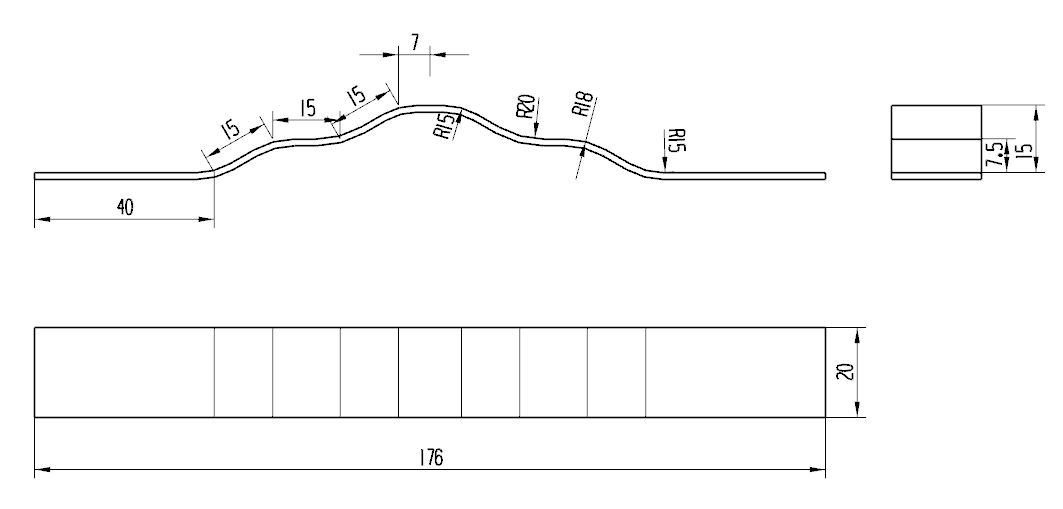
\includegraphics[width=0.9\textwidth]{./figs/fig-demensionofspecimen.png}}

\subfloat[Real specimen]{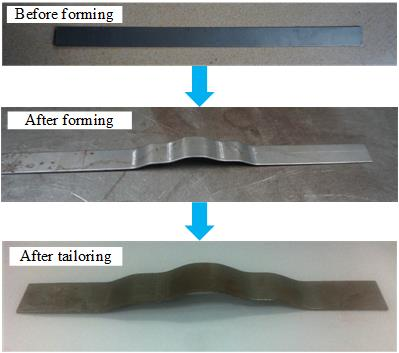
\includegraphics[width=0.9\textwidth]{./figs/forming.jpg}}

\caption{The specimen}
\label{fig:stampingformedspecimen}
\end{figure}

\subsection{Indentation test and Finite Element model}

To characterize the mechanical properties of the formed specimen above mentioned, the indentation test is adopted in this article. Since the formed specimen is symmetrical in both sides, one quarter of the specimen is studied in the article, which can be seen in Fig.~\ref{fig:measuredindentation}. The indentation tests are performed along the contour line of the specimen. The measured points are located every $1mm$ thus 55 points are measured in the indentation tests. In order to figure out the difference between the material properties of raw DP590 and that of formed specimen, a small plate cut from the raw DP590 was prepared, the dimension of which is $10mm \times 10mm \times 1.4mm$, and to avoid the affect of casual factors, three tests points were chosen randomly in the measurement domain, which can be seen from the Fig.~\ref{fig:measuredtension}.

\begin{figure}[h]
\centering
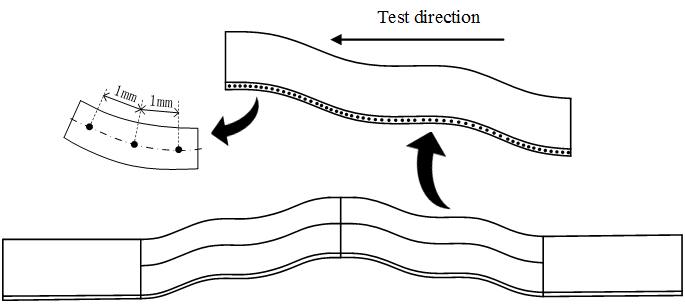
\includegraphics[width=0.8\textwidth]{./figs/Drawing2.png}
\caption{The measured points of indentation test}
\label{fig:measuredindentation}
\end{figure}

\begin{figure}[h]
\centering
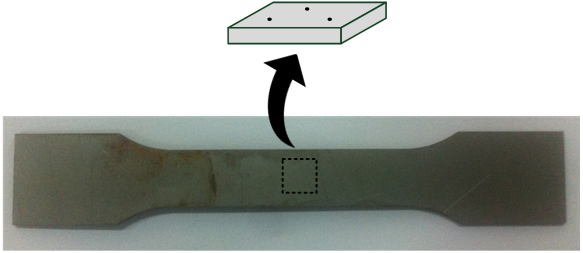
\includegraphics[width=0.9\textwidth]{./figs/Drawing3.png}
\caption{The measured points without formed}
\label{fig:measuredtension}
\end{figure}

Due to the size of one quarter of the formed specimen is too big to conduct the indentation test, different small slices were cut out from the formed specimen by water-jet. These slices then were mounted in epoxy cylindrical foundation. It is known that the surface has a significant influence on the indentation test results. Preparation of the test surface shall be carried out in such a way that any alteration of the surface hardness (e.g. due to heat or cold-working) is minimized. Therefore, the surface of specimen was ground with 400-2500 grit sandpapers and then polished by alumina suspension in order to obtain a flat and smooth surface..


The indentation tests were performed at room temperature using a TriboIndenter Test system (Hysitron Inc., USA). The machine operation conforms to the ISO 14577 and ASTM E2546-07 standards. The Berkovich indenter made of industrial diamond with an elastic modulus of $1141 Gpa$ and Poisson's ratio of 0.07 was employed. In all indentation tests, a triangular load history was prescribed, defined by a loading time of 5s, an unloading time of 5s, and without a holding time, and a fixed maximum displacement of 2 $um$ at a constant loading and unloading rate of $400nm/s$ was applied.

To investigate the constitutive properties of the formed specimen and indenting load to P-h curves of indentation, finite element (FE) analyses for conical indentation were carried out using the nonlinear finite element analysis program ABAQUS.

A conical rigid indenter with half-angle of $70.3^{\circ}$ was used in the model which has the same projected area to depth function as the standard Berkovich indenter. Due to that a 2-D simulation requires less computational time and is more convenient than a 3D model and there is very little difference between the results obtained from the 2-D axisymmetric and 3-D finite element simulations of the indentation experiment by Berkovich indenter, a 2-D axisymmetric model was employed for FE simulation of the elastic–plastic behavior of material in the microindentation process.

The specimen was meshed with 42050 linear axisymmetric triangular elements (CAX3R in ABAQUS) as shown in Fig.~\ref{fig:FEm}. A fine mesh near the contact region and a gradually coarser mesh further from the contact region were designed to ensure numerical accuracy and save computational time. At the maximum displacement, the minimum number of contact elements in the contact zone was ensured to have not less than 16 elements in each FE analysis.

\begin{figure}[h!]
\centering
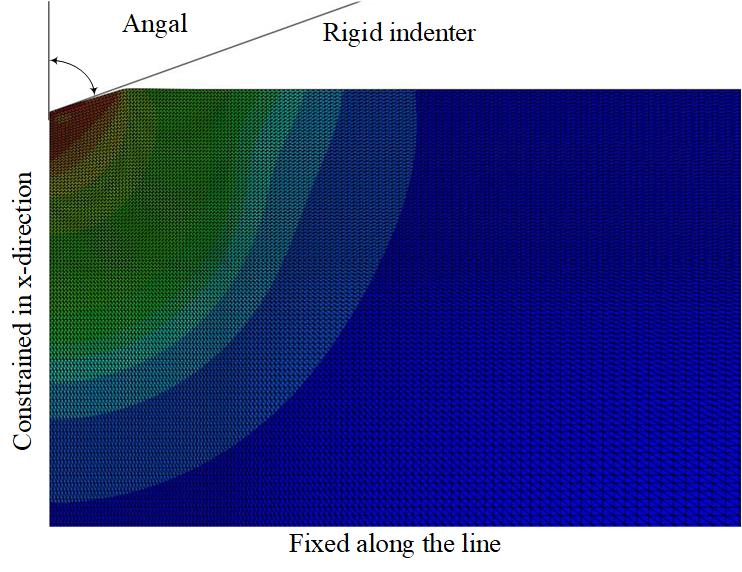
\includegraphics[width=0.95\textwidth]{./figs/FEMindention.jpg}
\caption{The FE model of indentation test (angle = $70.3^{\circ}$)}
\label{fig:FEm}
\end{figure}

Loading steps of micro-indentation process is simulated in the FE model, which is correlated with the indentation test. During the loading stage, the indenter was driven into the specimen surface in the axial direction for $2um$ in 5s and with a constant speed.

The geometric boundary conditions were applied as follows: the nodes along y axis (the axis of rotation) can move only along the axis itself and all the nodes on the bottom of the mesh were fixed. The indenter was modeled as a rigid movable surface and the contact between the indenter and the matrix surface was assumed to be frictionless based on Bucaille's study \cite{bucaille2003determination}. Due to quasi-static nature, the mass inertial effect is neglected. Residual stresses are not taken into account in the present FE model.

\subsection{Digital image correlation test setup and procedure}

Image analysis technique, such as 3D Digital Image Correlation (DIC), can provide full-field responses which also contains the local material properties of the formed specimen. In this study, this technique is used to verify the material properties identified by indentation tests. To eliminate the effects of casual factors, 5 formed specimens are manufactured. The experimental platform is presented in Fig.\ref{fig:DICplatform}. The types of devices shown in Fig.\ref{fig:DICplatform} is presented in Table.\ref{table:DIC}.

\textcolor{black}{Before testing, the formed specimens firstly are polished. Then these polished specimens are wiped with anhydrous alcohol to clean the small particles and rusty spots. After that, the specimens are spray painted with white undercoat then black matte ink. At last, the specimen with uniform speckle are obtained for DIC test.}

\begin{table}[h!]
\centering
\caption{The device of DIC}
\begin{tabular}{c c c} 
 \hline
 - & Device or software & Function\\
 \hline
 \multirow{3}{4em}{Hardware} &  CCD Camera (2 million pixels) & Collect Images\\ 
& LED light (220V 150W) & provide light  \\
& Control computer (3.5GHz CPU) & control test \\
\multirow{2}{4em}{Soltware} & VIC-Snap & Image capture \\
& VIC-Analysis & Image processing \\
 \hline
\end{tabular}
\label{table:DIC}
\end{table}


\begin{figure}[h!]
\centering
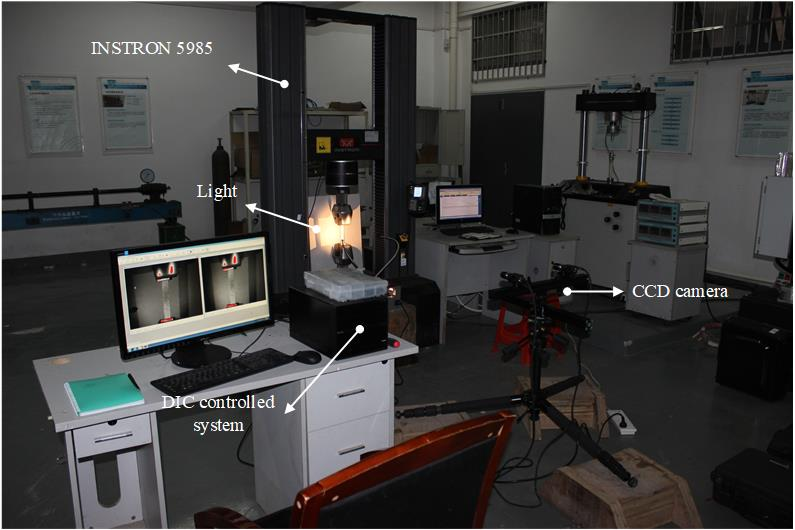
\includegraphics[width=1\textwidth]{./figs/DIC.jpg}
\caption{The DIC platform}
\label{fig:DICplatform}
\end{figure}

\section{Approximate Bayesian computation}

Due to its flexibility, Bayesian framework has been widely used in the inverse problems. It can regularize the ill-posed inverse problem with the prior information. Thus, stable results can be obtained. The formula of it is

\begin{equation}
\label{eq:bayesian}
p(\mathbf{\Theta} | \mathbf{Y}_{obs}) = k \cdot p(\mathbf{\Theta}) \cdot p( \mathbf{Y}_{obs} | \mathbf{\Theta} )
\end{equation}

\noindent where $\mathbf{\Theta}$ denotes the material parameter vector, $p(\mathbf{\Theta})$ is its prior distribution which is from the known or given information, $\mathbf{Y}_{obs}$ is the measured experimental data,  $p(\mathbf{Y}_{obs}|\mathbf{\Theta})$ is its likelihood function which denotes the experimental information and $k$ is the normalized constant which can make the integral of right term equal to 1. Since the constant is independent with $\mathbf{\Theta}$, it can ignore in Eq.\ref{eq:bayesian}. Thus the Eq.\ref{eq:bayesian} can be rewritten as 

\begin{equation}
\label{eq.bayesianratiao}
p(\mathbf{\Theta} | \mathbf{Y}_{obs}) \propto p(\mathbf{\Theta}) \cdot p( \mathbf{Y}_{obs} | \mathbf{\Theta})
\end{equation}

\subsection{The basic theory of ABC}

However in the engineering practice, the likelihood function of Bayesian framework is always intractable. Fortunately, an approximate Bayesian computation (ABC) \cite{pritchard1999population} is proposed. It can circumvent the intractable likelihood function via two steps of approximation \cite{blum2013comparative}. At first step, in order to avoid of the curse of dimensionality of observations, the observations $\mathbf{Y}_{obs}$ in Eq.~\ref{eq.bayesianratiao} is approximated by its summary statistics, then it has

\begin{equation}
\label{eq:firstapproximate}
p(\mathbf{\Theta} | \mathbf{Y}_{obs}) \approx p(\mathbf{\Theta} | S(\mathbf{Y}_{obs})) \propto p(\mathbf{\Theta})\cdot p( S(\mathbf{Y}_{obs}) | \mathbf{\Theta})
\end{equation}

\noindent where $S(\mathbf{Y}_{obs})$ is the observations' summary statistics whose dimension is much lower than that of $\mathbf{Y}_{obs}$. However, $p(S(\mathbf{Y}_{obs}) | \theta)$ may be still computationally intractable in practice. A second approximation is utilized:

\begin{equation}
\label{eq:secondapproximate}
p \left( S_{obs} | \mathbf{\Theta}  \right) = p \left(  S(\mathbf{Y}_{obs} = \mathbf{Y}_{sim})  | \mathbf{\Theta} \right) \approx p \left( \Vert S(\mathbf{Y}_{obs}), S(\mathbf{Y}_{sim}) \Vert \leq \epsilon | \mathbf{\Theta} \right)
\end{equation}

\noindent where $\mathbf{Y}_{sim}$ is from simulation of sample, $\Vert \cdot \Vert$ is the distance measure mostly euclidean distance, $\epsilon \geq 0$ is scale parameter. From Eq.~\ref{eq:secondapproximate}, it can shown that if $\epsilon=0$, the ``$\approx$'' will change to ``$=$''. 

\section{POD theory and  POD-based ABC}

According to Blum \cite{blum2013comparative}, a trade-off of summary statistics should be reached. If the number of statistics is too large, the statistics is summary and can contain almost all information of observations, then the first step of approximation can be satisfied well. However, for the second step of approximation it is inefficient to sample the $S(\mathbf{Y}_{sim})$ which can satisfy the distance measure $\epsilon$ in high dimensional space. Conversely, if the number is too small, it is efficient to satisfy the distance measure in the second approximation. However, the smaller the number of statistics is, the less information these statistics contain. This will lead to poor approximation in Eq.\ref{eq:firstapproximate}. Then a trade-off of selection of the statistics should be reached. However, it is always difficult to achieve this trade-off in practice. The POD is widely used dimensional reduction method. It can convert the high-dimensional observations to low-dimensional coefficient vector with little information lost. In this study, we extend the POD into ABC and proposed a feasible and flexible POD-based ABC framework.

In this section, we will introduce the POD theory briefly firstly and then shown how it works in ABC. 

\subsection{POD theory}

At the beginning, suppose that $M$ snapshots are given. Suppose that in the matrix $\mathbf{Y}$, the column vector $\mathbf{Y}^j, j = 1,\cdots,M$ contains N observational points which is calculated by FE simulation given the $j-th$ parameter vector. Then $\mathbf{Y}$ is $N \times M$ matrix. Define the matrix $\mathbf{U}$ as

\begin{equation}
\label{eq:covariancematrix}
\mathbf{U} = \mathbf{Y}^T\mathbf{Y}
\end{equation}

It is obvious that $\mathbf{U}$ is the positive definite matrix. Thus, we can determine its eigenvalue matrix and eigenvector matrix with

\begin{equation}
\label{eq:eigenequation}
\mathbf{U}\cdot \mathbf{V} = \mathbf{\Lambda} \cdot \mathbf{V}
\end{equation}

\noindent where $\mathbf{V}$ is the eigenvector matrix of $\mathbf{U}$, $\mathbf{\Lambda}$ is diagonal matrix with positive descending order eigenvalues $\lambda_i$. We define the basis vector as

\begin{equation}
\label{eq:PODbasis}
\mathbf{\Phi} = \mathbf{Y}\cdot \mathbf{V}
\end{equation}

Due to the positive definite matrix $\mathbf{U}$, $\mathbf{V}$ is orthogonal, thus it has

\begin{equation}
\label{eq:orthogonal}
\mathbf{\Phi}^T \cdot \mathbf{\Phi}
= \mathbf{V}^T \cdot \mathbf{U} \cdot \mathbf{V} =\mathbf{V}^T \cdot \mathbf{\Lambda} \cdot \mathbf{V}= \mathbf{I}
\end{equation}

According to \cite{berkooz1993proper}, eigenvalues are defined as the measure of kinetic energy transferred of the basis vectors. The rapid descending eigenvalues mean that the kinetic energy will decrease rapidly. This permits us discarding part of basis vector. Thus based on the fraction of the kinetic energy, the POD basis $\mathbf{\Phi}$ is truncated to $\mathbf{\bar{\Phi}}$ which is $N \times K$ matrix ($K < N$). For every snapshot, it can express as 

\begin{equation}
\label{eq:PODtrunaxted}
\mathbf{Y} ^ j \approx  \mathbf{\bar{\Phi}} \cdot \mathbf{B}^j
\end{equation}

\noindent where $\mathbf{B}_j = [\beta_1^j,\beta_2^j,\ldots,\beta_K^j ]$ is the unknown coefficient vector and for the snapshots, its coefficient vector can be determined as 

\begin{equation}
\label{eq:coefficient of POD}
\mathbf{\bar{B}} = \mathbf{\bar{\Phi}}^T \cdot \mathbf{Y}
\end{equation}

As for the observations, it can be approximated as

\begin{equation}
\label{eq:observation of POD}
\mathbf{Y}_{obs} = \mathbf{\bar{\Phi}} \cdot \mathbf{B}_{obs}
\end{equation}

\noindent where the coefficient vector $\mathbf{B}_{obs}$ can be determined by least square fit or weighted residuals. 

\subsection{POD-based ABC framework}

From the theory above, it can be shown that the observations can be express as a linear combination of truncated POD basis vectors. Thus after the basis vectors are determined, the high-dimensional observations can be transferred to its coefficient vectors with little information lost. Since the kinetic energy decrease rapidly mentioned before, the dimension of the coefficient vector is far less than that of observations. This provide us a shortcut in ABC instead of selection of statistics. Based on Eq.\ref{eq:observation of POD} the first approximation Eq.\ref{eq:firstapproximate} can be rewritten as 

\begin{equation}
\label{eq:PODfirstapprox}
p(\mathbf{\Theta}|\mathbf{Y}_{obs}) \approx p(\mathbf{\Theta}| \mathbf{\bar{\Phi}} \mathbf{B}_{obs})
\end{equation}

Thus, the second approximation of ABC can be written as 

\begin{equation}
\label{eq:PODsecondapprox}
p\left( \mathbf{\bar{\Phi}} \mathbf{B}_{obs} | \mathbf{\Theta} \right) \approx p\left( \Vert \mathbf{\bar{\Phi}} \mathbf{B}_{obs}, \mathbf{\bar{\Phi}} \mathbf{B} \Vert \leq \epsilon | \mathbf{\Theta} \right)
\end{equation}

\noindent where $\mathbf{\bar{\Phi}} \mathbf{B}$ is from simulation. Since for a given field, the basis vectors are constant, the observation is just a linear function of the coefficient vector based on Eq.\ref{eq:observation of POD}. Thus the right term of Eq.\ref{eq:PODsecondapprox} can be extended as 

\begin{equation}
\label{eq:abcpod}
p\left( \Vert \mathbf{\bar{\Phi}} \mathbf{B}_{obs}, \mathbf{\bar{\Phi}} \mathbf{B} \Vert \leq \epsilon | \mathbf{\Theta} \right) = p \left(\Vert \mathbf{B}_{obs}, \mathbf{B} \Vert \leq \epsilon _\mathbf{B} | \mathbf{\Theta} \right)
\end{equation}

\noindent where $\epsilon _\mathbf{B}$ is still a small value for a new distant measure of coefficient vector. If $\epsilon _\mathbf{B}$ equals to 0, the ``$\approx$'' of Eq.\ref{eq:PODsecondapprox} can also change to ``$=$''. 

However, obtaining simulated coefficient vector given a parameter vector is very time-consuming, since at first we need to implement the FE simulation to obtain the response and then obtain coefficient vector based on Eq.\ref{eq:coefficient of POD}. The FE simulation is time-consuming. And for ABC, numerous samples are needed. This will lead to prohibitive computation.

In order to address this issue, we regard the coefficient vector is a non-linear function of the material parameters. The feed-forward Neural Network(NN) is used to construct the non-linear connection between material parameter vector and the coefficient vector. Via NN, we can obtain the coefficient vector $\mathbf{B}$ efficiently when the material parameters are given.

NN is an excellent tool \cite{li2016identification} to construct the complex non-linear relationship between input and output in engineering. The detail is referred to \cite{bishop2006pattern}. The construction of single hidden layer NN used in this study is shown in Fig.~\ref{fig:NN}. According to the feed-forward NN \cite{bishop2006pattern}, we can construct the connection between parameters and coefficient vectors as

\begin{equation}
\label{eq:NN}
\beta_k(\mathbf{\Theta},\mathbf{W})= \sigma \left( \sum_{j=1}^S w_{kj}^{(2)} h \left( \sum_{i=1}^D w_{ji}^{(1)} \theta_i + b_{j}^{(1)} \right) + b_{k}^{(2)} \right)
\end{equation}

\noindent where $\mathbf{\Theta} = [\theta_1,...,\theta_D]$, $w_{ji}^{(1)}$ is the weight of first layer, $b_{j}^{(1)}$ is its bias, $w_{kj}^{(2)}$ is the weight of second layer, $b_{k}^{(2)}$ is its bias, $h(\cdot)$ is called hidden units and an activation function which is nonlinear such as logistic sigmoid or `tanh' function. This nonlinear activation function is very important. Without it, the relationship between parameters and coefficient vector can be linear. This will limit the application of NN. The choice of it is discussed in detail in \cite{bishop2006pattern}. In this study, snapshots are used as the training data of NN. Here our goal is to replace the observation with combination of POD truncated basis, compared with popular NN, the feature of error function of NN here is a little different. The error function is defined as

\begin{equation}
  L(\mathbf{W}) = \sum_{n=1}^M \Vert \bar{\mathbf{\Phi}} \cdot \mathbf{B} (\mathbf{\Theta}_n,\mathbf{W})-\mathbf{Y}_n \Vert ^2
\end{equation}

\begin{figure}[h!]
\centering
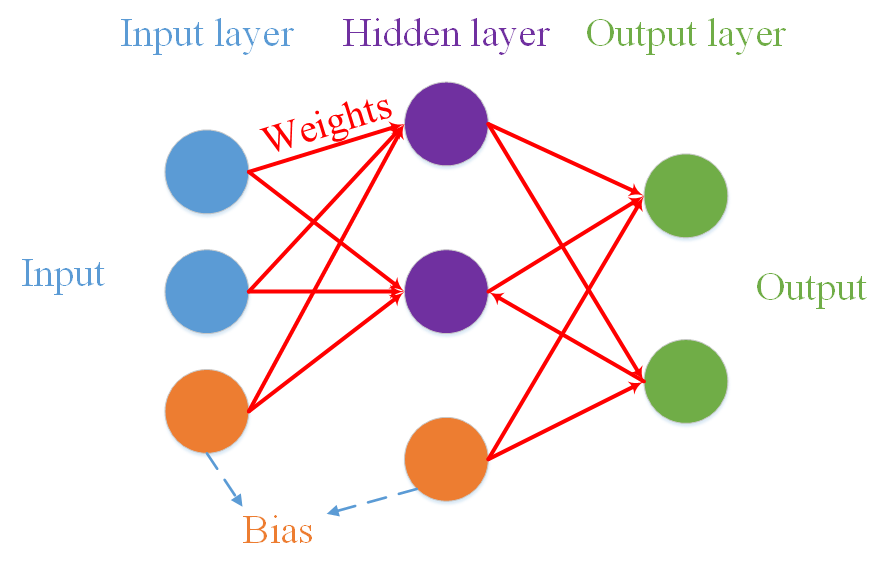
\includegraphics[width=1\textwidth]{./figs/NN.png}
\caption{The construction of neural network}
\label{fig:NN}
\end{figure}

Via minimizing the error function, all the parameters of NN can be determined. In order to measure the goodness of the POD and NN, the $R^2$ is used, it has

\begin{equation}
R^2 = 1-\frac{\sum_{i=1}^t \Vert \mathbf{y}_i - \tilde{\mathbf{y}}_i \Vert ^2 }{\sum_{i=1}^t \Vert \mathbf{y}_i - \bar{\mathbf{y}}_i \Vert ^2}
\end{equation}

\noindent where $t$ is the number of test samples, $\mathbf{y}_i$, $\tilde{\mathbf{y}}_i$, $\bar{\mathbf{y}}_i$ are the FE response, the mean of FE response, and the response calculated with the POD basis and the coefficient vector determined by NN given the test samples. If $R^2$ approaches 1, it means the accuracy of proposed method approaches the FE response. After the performance of POD and NN is verified, it means that the coefficient vector determined by NN is accurate enough to replace the FE simulation. Then given parameter vector, it is easy to get its simulated coefficient vector with the well-constructed NN. \textcolor{black}{In this study, since the inputs and outputs of are low dimensional, one hidden layer with 10 neurons is used.} 

Based on two steps of approximation in Eqs.\ref{eq:PODfirstapprox},\ref{eq:PODsecondapprox},\ref{eq:abcpod}, the POD-based ABC make use of comparisons between simulated and observed coefficient vector of POD to determine the material parameters efficiently. It is obvious that the summary statistics are replaced by the coefficient vector of POD in the POD-based ABC. Thus, the complex selection of summary statistics of ABC is circumvented by the POD-based ABC framework. Furthermore, with the well-constructed NN, the proposed method can obtain the simulated coefficient vector without time-consuming FE simulation. Thus, the proposed method is flexible and feasible.

\subsection{Sampling}
Sampling method is also very important method. Pritchard \cite{pritchard1999population} proposed ABC with a rejection method. In this method, if prior is quite different with the posterior, it will reject majority of the samples. The efficiency can be very low. To address this problem, the MCMC \cite{marjoram2003markov}, PMC \cite{beaumont2009adaptive,beaumont2010approximate}, SMC \cite{toni2009approximate}, PRC \cite{sisson2007sequential} are extended in ABC. 

In the ABC-PMC \cite{beaumont2009adaptive,beaumont2010approximate}, we first given the decreasing sequence of measure distant $\epsilon_t, (1 \leq t \leq T)$. In initial step, the sample $\mathbf{\Theta}^{(t)}$ derives from the prior distribution $p(\mathbf{\Theta})$. In arbitrary step $t (t > 1)$, we sample $\mathbf{\Theta}^{(t)}$ from an Gaussian Markov transition kernel $q(\mathbf{\Theta} | \mathbf{\Theta}^*)$ where $\mathbf{\Theta}^*$ is sampled from $\mathbf{\Theta}^{(t-1)}$ with the weights $w_i^{(t-1)},i = 1,\cdots, N$. Then $\mathbf{\Theta}^{(t)}$ is accepted with $\Vert \mathbf{B}_{obs}, \mathbf{B}(\mathbf{\Theta}^{(t)}) \Vert \leq \epsilon$. In the PMC, the Gaussian kernel is adaptive which its mean is $\mathbf{\Theta}^{(t-1)}$ and variance is twice the weighted empirical variance of lats step sample $\mathbf{\Theta}^{(t-1)}$. The weight is given as

\begin{equation}
\label{eq:weight of PMC}
w_i^t \propto \frac{p(\mathbf{\Theta}_i^t)}{\sum_{j=1}^N w_j^{t-1} q(\mathbf{\Theta}_i^t | \mathbf{\Theta}_j^{t-1})}
\end{equation}

In the ABC-PMC, all things are deterministic except the decreasing sequence of measure distant $\epsilon_t, (1 \leq t \leq T)$. It is critical for the efficiency of PMC. The ABC-NPMC \cite{zeng2017} can determine them adaptively and can reach a rather high efficiency. Therefore, the ABC-NPMC is used here. The detail refers to  \cite{zeng2017}.

\subsection{Flowchart}
\textcolor{black}{
As shown in Fig.~\ref{fig:flowchart}, the flowchart of the proposed method is:
\begin{itemize}
\item[a.] Generate snapshot samples and test samples in the parameters' space.
\item[b.] Complete indentation FE simulations with  snapshot samples and test samples.
\item[c.] Based on the P-h curves calculated by FE simulations, the POD basis vector and coefficient vector of parameter samples are calculated according to the POD theory mentioned in Sec.4.1. Identify the observed coefficient vector.
\item[d.] Construct NN with the snapshot samples and the coefficient vector
\item[e.] The accuracies of POD and NN are verified by the test samples. If accuracy is not enough, add more sample and the procedure goes back to \textbf{Step a}.
\item[f.] Complete the ABC calculation with the comparison between sampled and observed coefficient vector.
\end{itemize}
}
\begin{figure}[h]
\centering
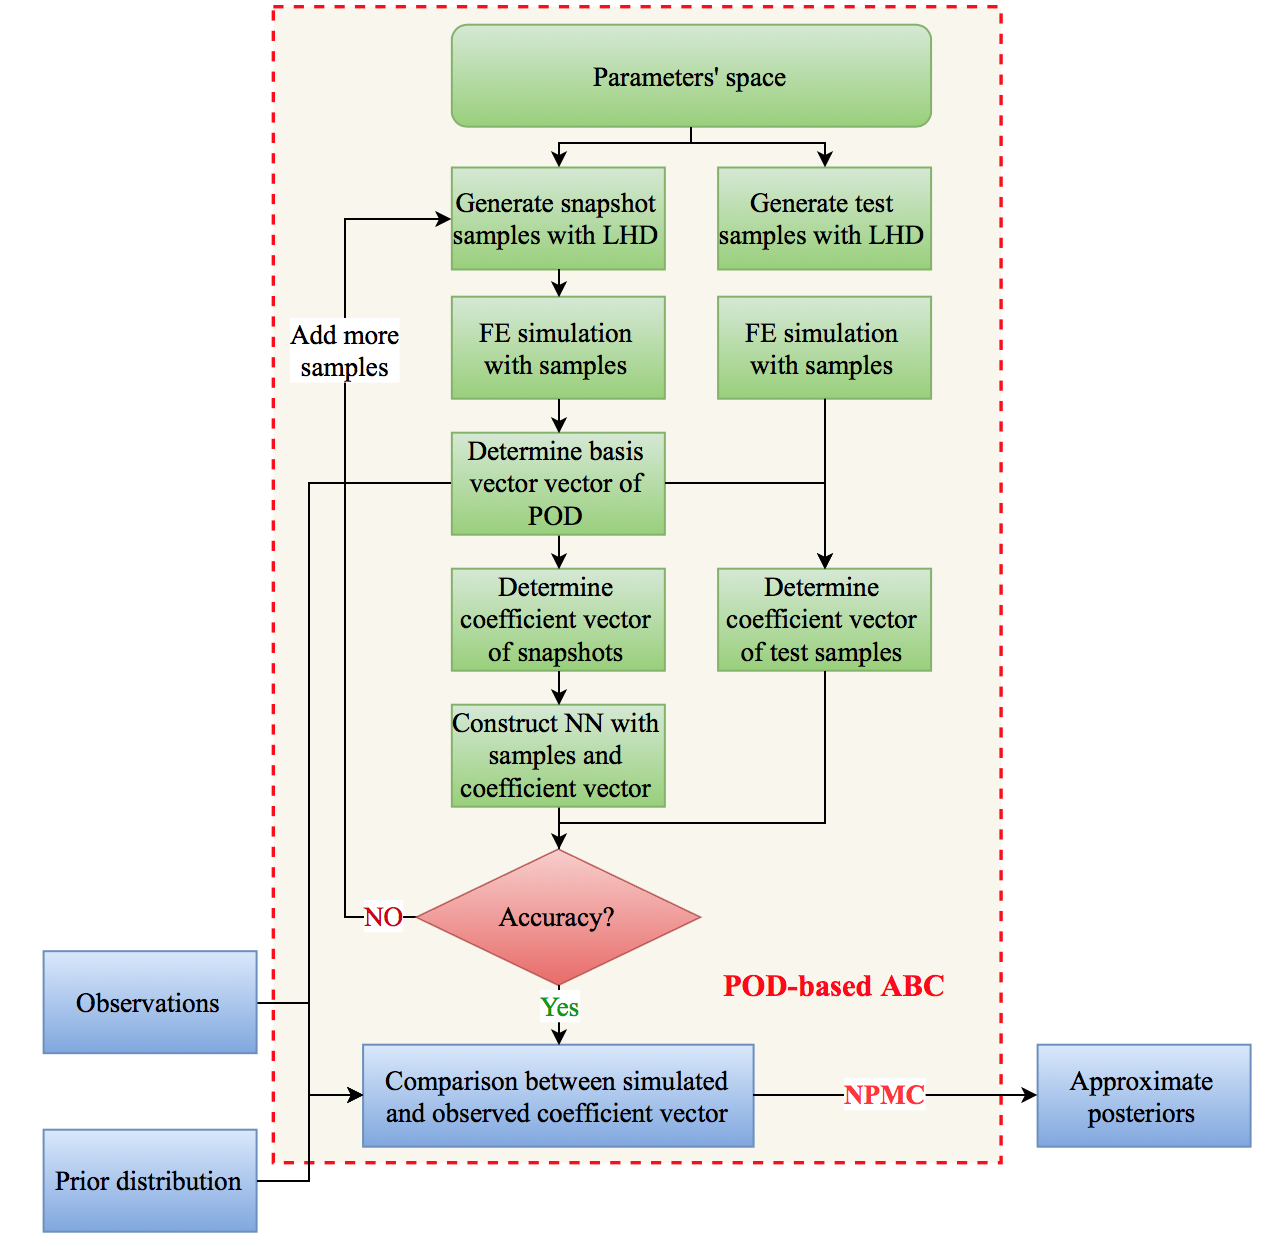
\includegraphics[width=1\textwidth]{./figs/flowchart.png}
\caption{The flowchart of POD-based ABC}
\label{fig:flowchart}
\end{figure}

\section{Results}

\subsection{Results of indentation tests}

The hardness of the measured points as shown in Fig.\ref{fig:hardness} is calculated by relations which have been derived from the theory of contact mechanics and the Oliver–Pharr’s method \cite{oliver1992improved}. It can be shown that the fluctuation of the hardness is quite large: the largest value of hardness is over 20\% larger than the smallest one.

\begin{figure}[h!]
\centering

\subfloat[The hardness of the indentation test]{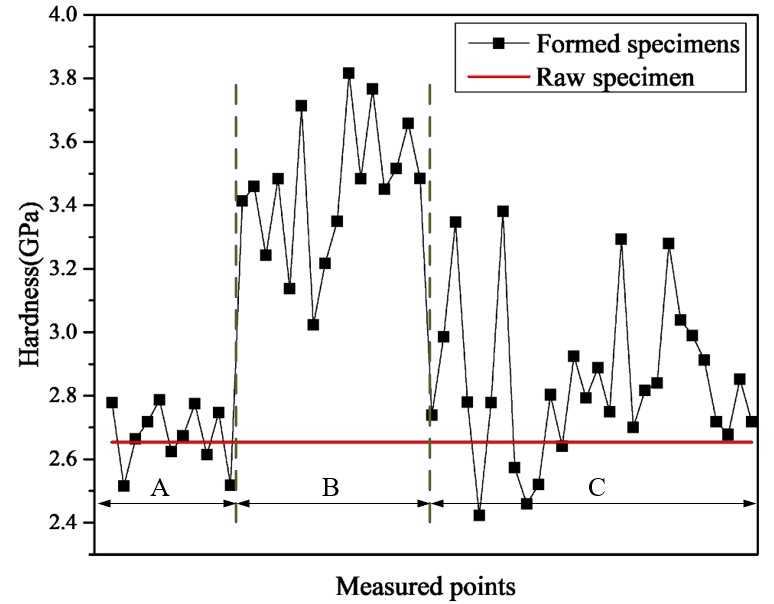
\includegraphics[width=0.8\textwidth]{./figs/hardness3.png}}

\subfloat[The partition of the specimen]{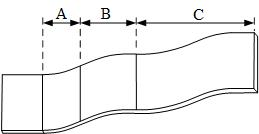
\includegraphics[width=0.6\textwidth]{./figs/partitioned.jpg}}
\caption{The hardness of indentation test and partition}
\label{fig:hardness}
\end{figure}

Identifying parameter properties for all points is not necessary, since it is very time-consuming even prohibitive to implement FE simulation with numerous parameter properties. Furthermore, for single observations, there may be some casual factor such as measurement error which can lead to inaccurate simulation. Therefore, based the feature of hardness as shown in Fig.~\ref{fig:hardness}a, we can divide the observations as three regions which separately labeled as A, B and C as shown in Fig.~\ref{fig:hardness}b. And each region has different measured points, the number of which are separately 11, 16 and 28 orderly as shown in Fig.~\ref{fig:hardness}b. \textcolor{black}{The difference of the hardness value of different region results from cold hardening of forming. This is similar with the work in Ref.\cite{sun2014determination}. As shown in Fig.~\ref{fig:hardness}b, the region A is the edge of forming. The deformation in this region is small. Thus the value of hardness in this region approaches that of raw specimen. From Fig.~\ref{fig:hardness}b, it can be shown that the main deformation of the forming is in region B. This lead to the value of hardness in region B is over 20\% larger than that of the raw DP590. As for region C, the influence of forming is very complicated. This leads to large deformation at some measured points and small deformation at the others. This is why the value of hardness in region C has a large fluctuation. In conclusion, from the value of hardness, the forming has a big influence on the mechanical properties.}

The P-h curves of the raw specimens are presented in Fig.~\ref{fig:rawDP590}. The P-h curves of three formed regions are presented in Fig.~\ref{fig:phcurve region}. These curves are consistent with value of the hardness in Fig.~\ref{fig:hardness}. On one hand, the less oscillation the value of hardness is, the more concentrated P-h curves are. On the other hand, the means of P-h curves in each region as shown in Fig.\ref{fig:phcurve region}e match the feature of hardness very well. This means of P-h curve in each region are used to characterize the mechanical properties of each region with proposed method. 

\begin{figure}[h!]
\centering
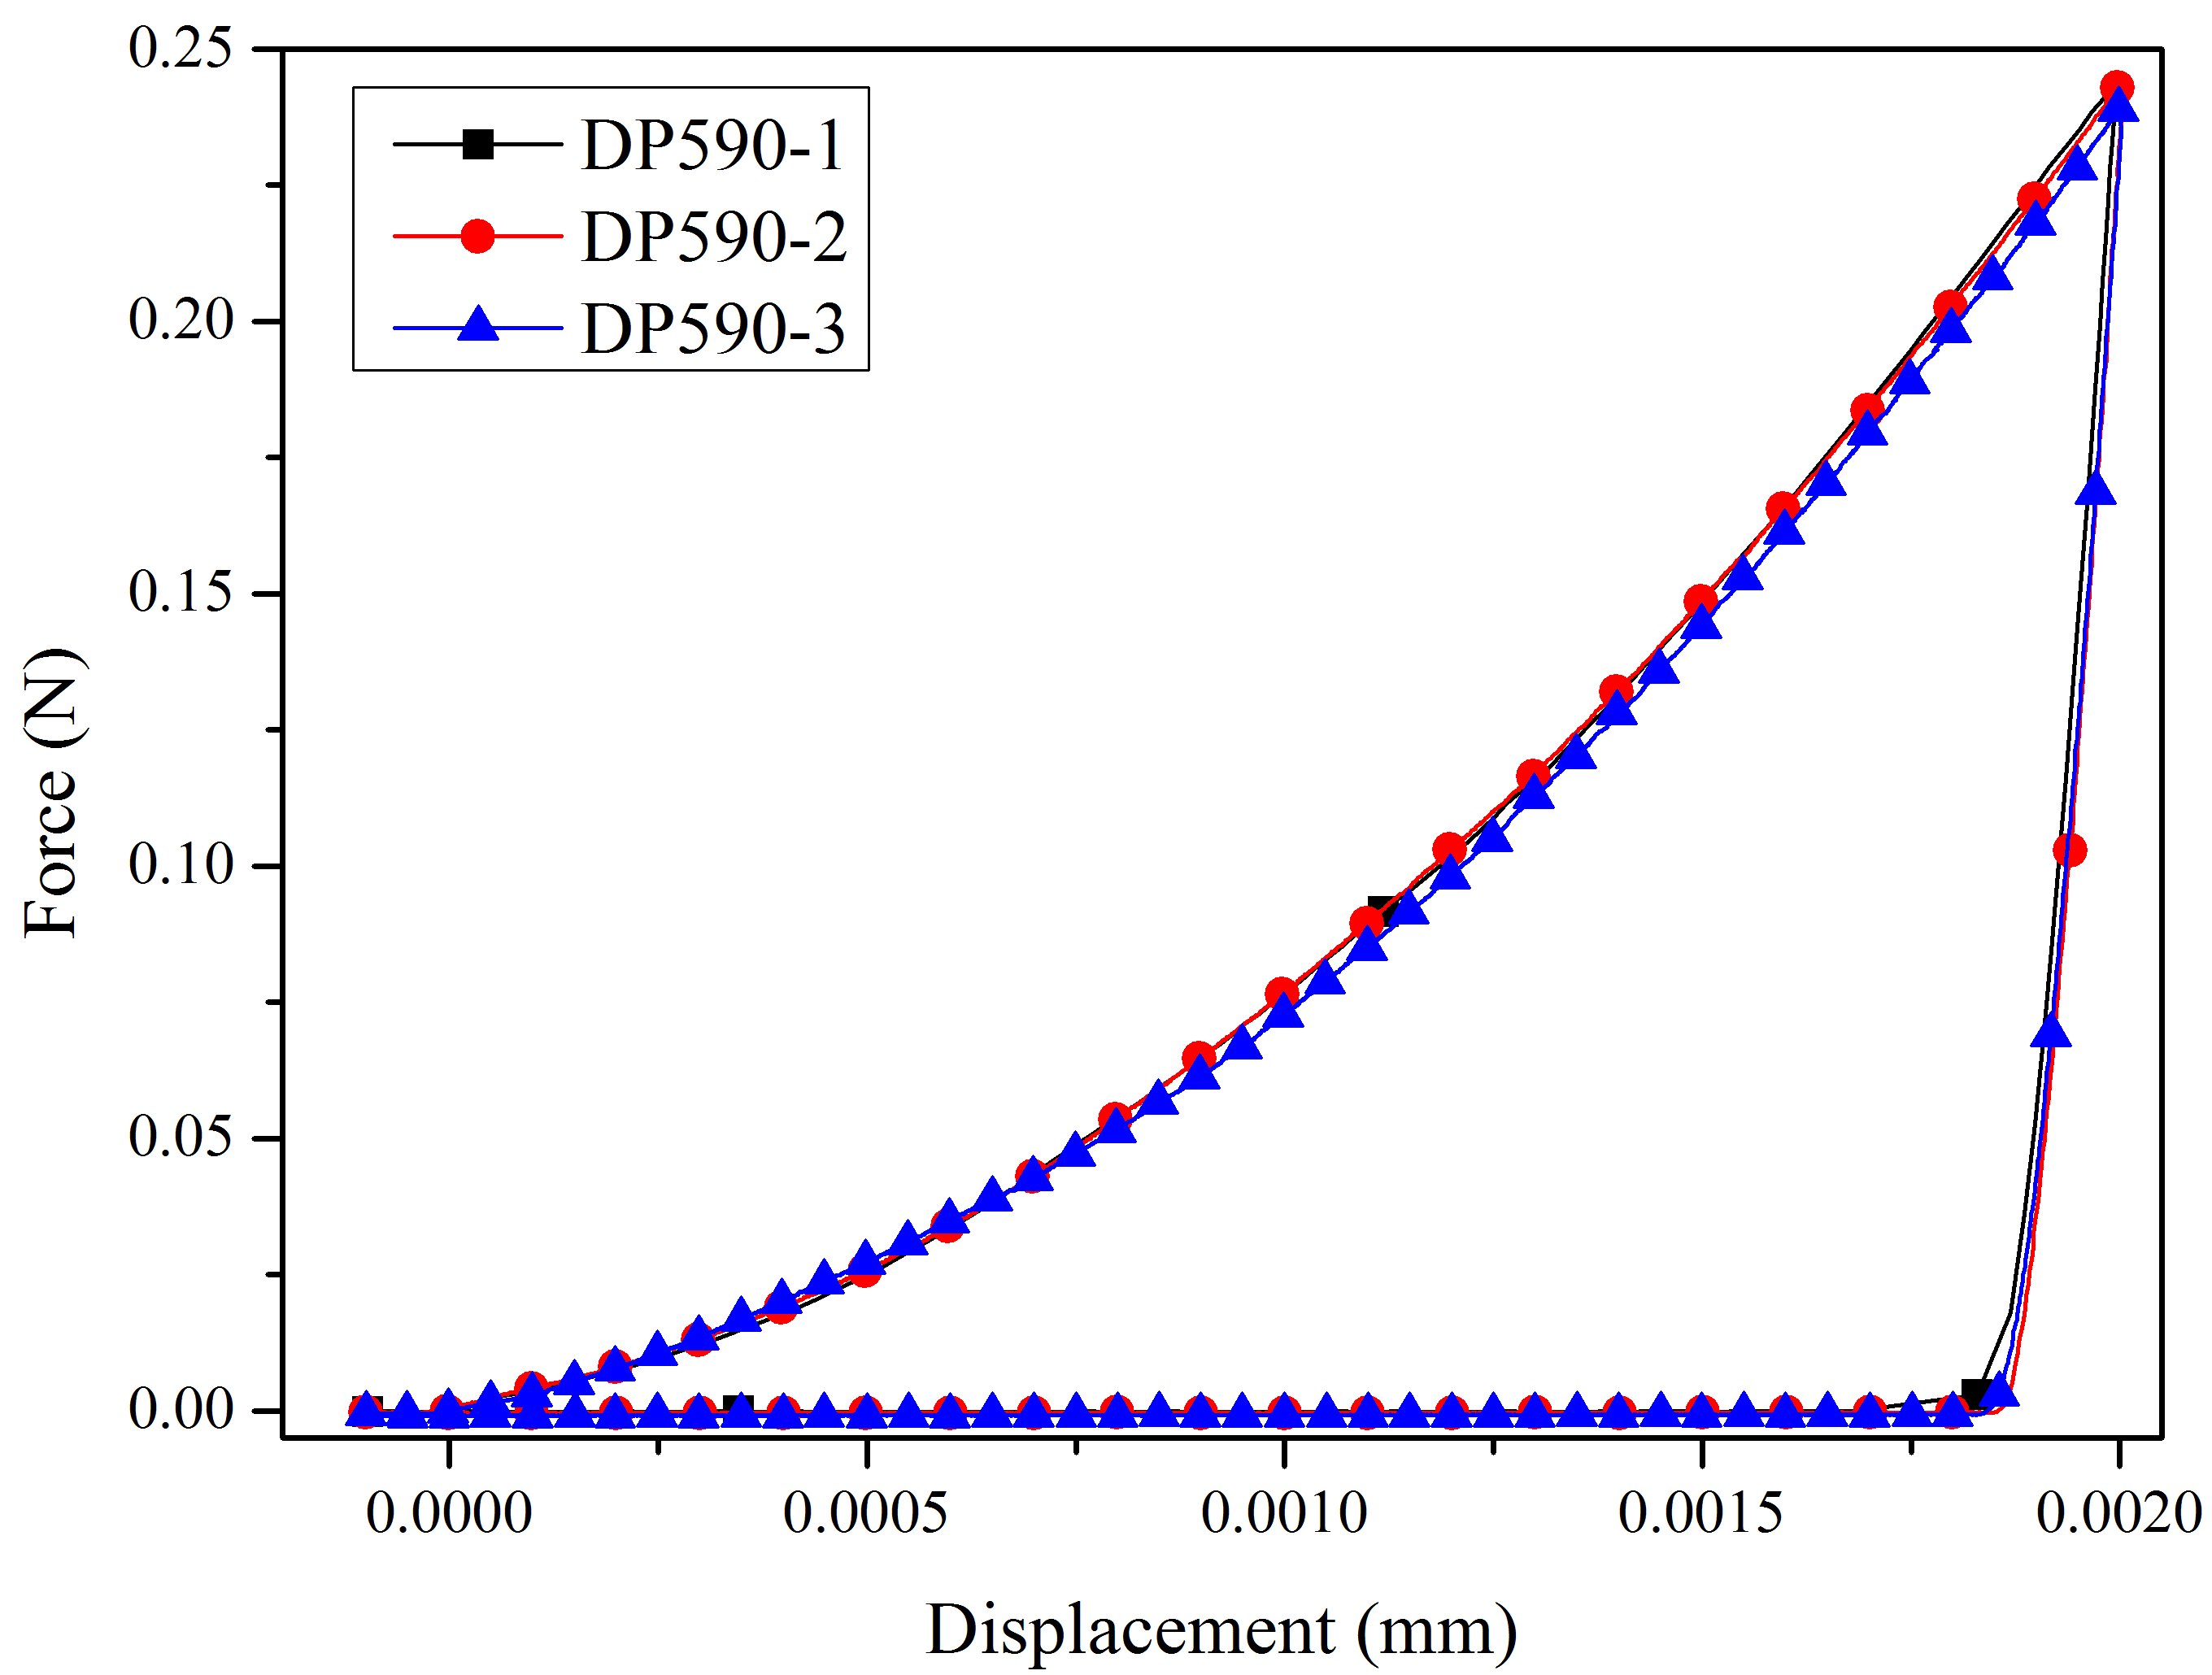
\includegraphics[width=0.7\textwidth]{./figs/DP590.png}
\caption{The P-h curve of raw specimen}
\label{fig:rawDP590}
\end{figure}

\begin{figure}[h!]
\centering
\subfloat[P-h curve of region A]{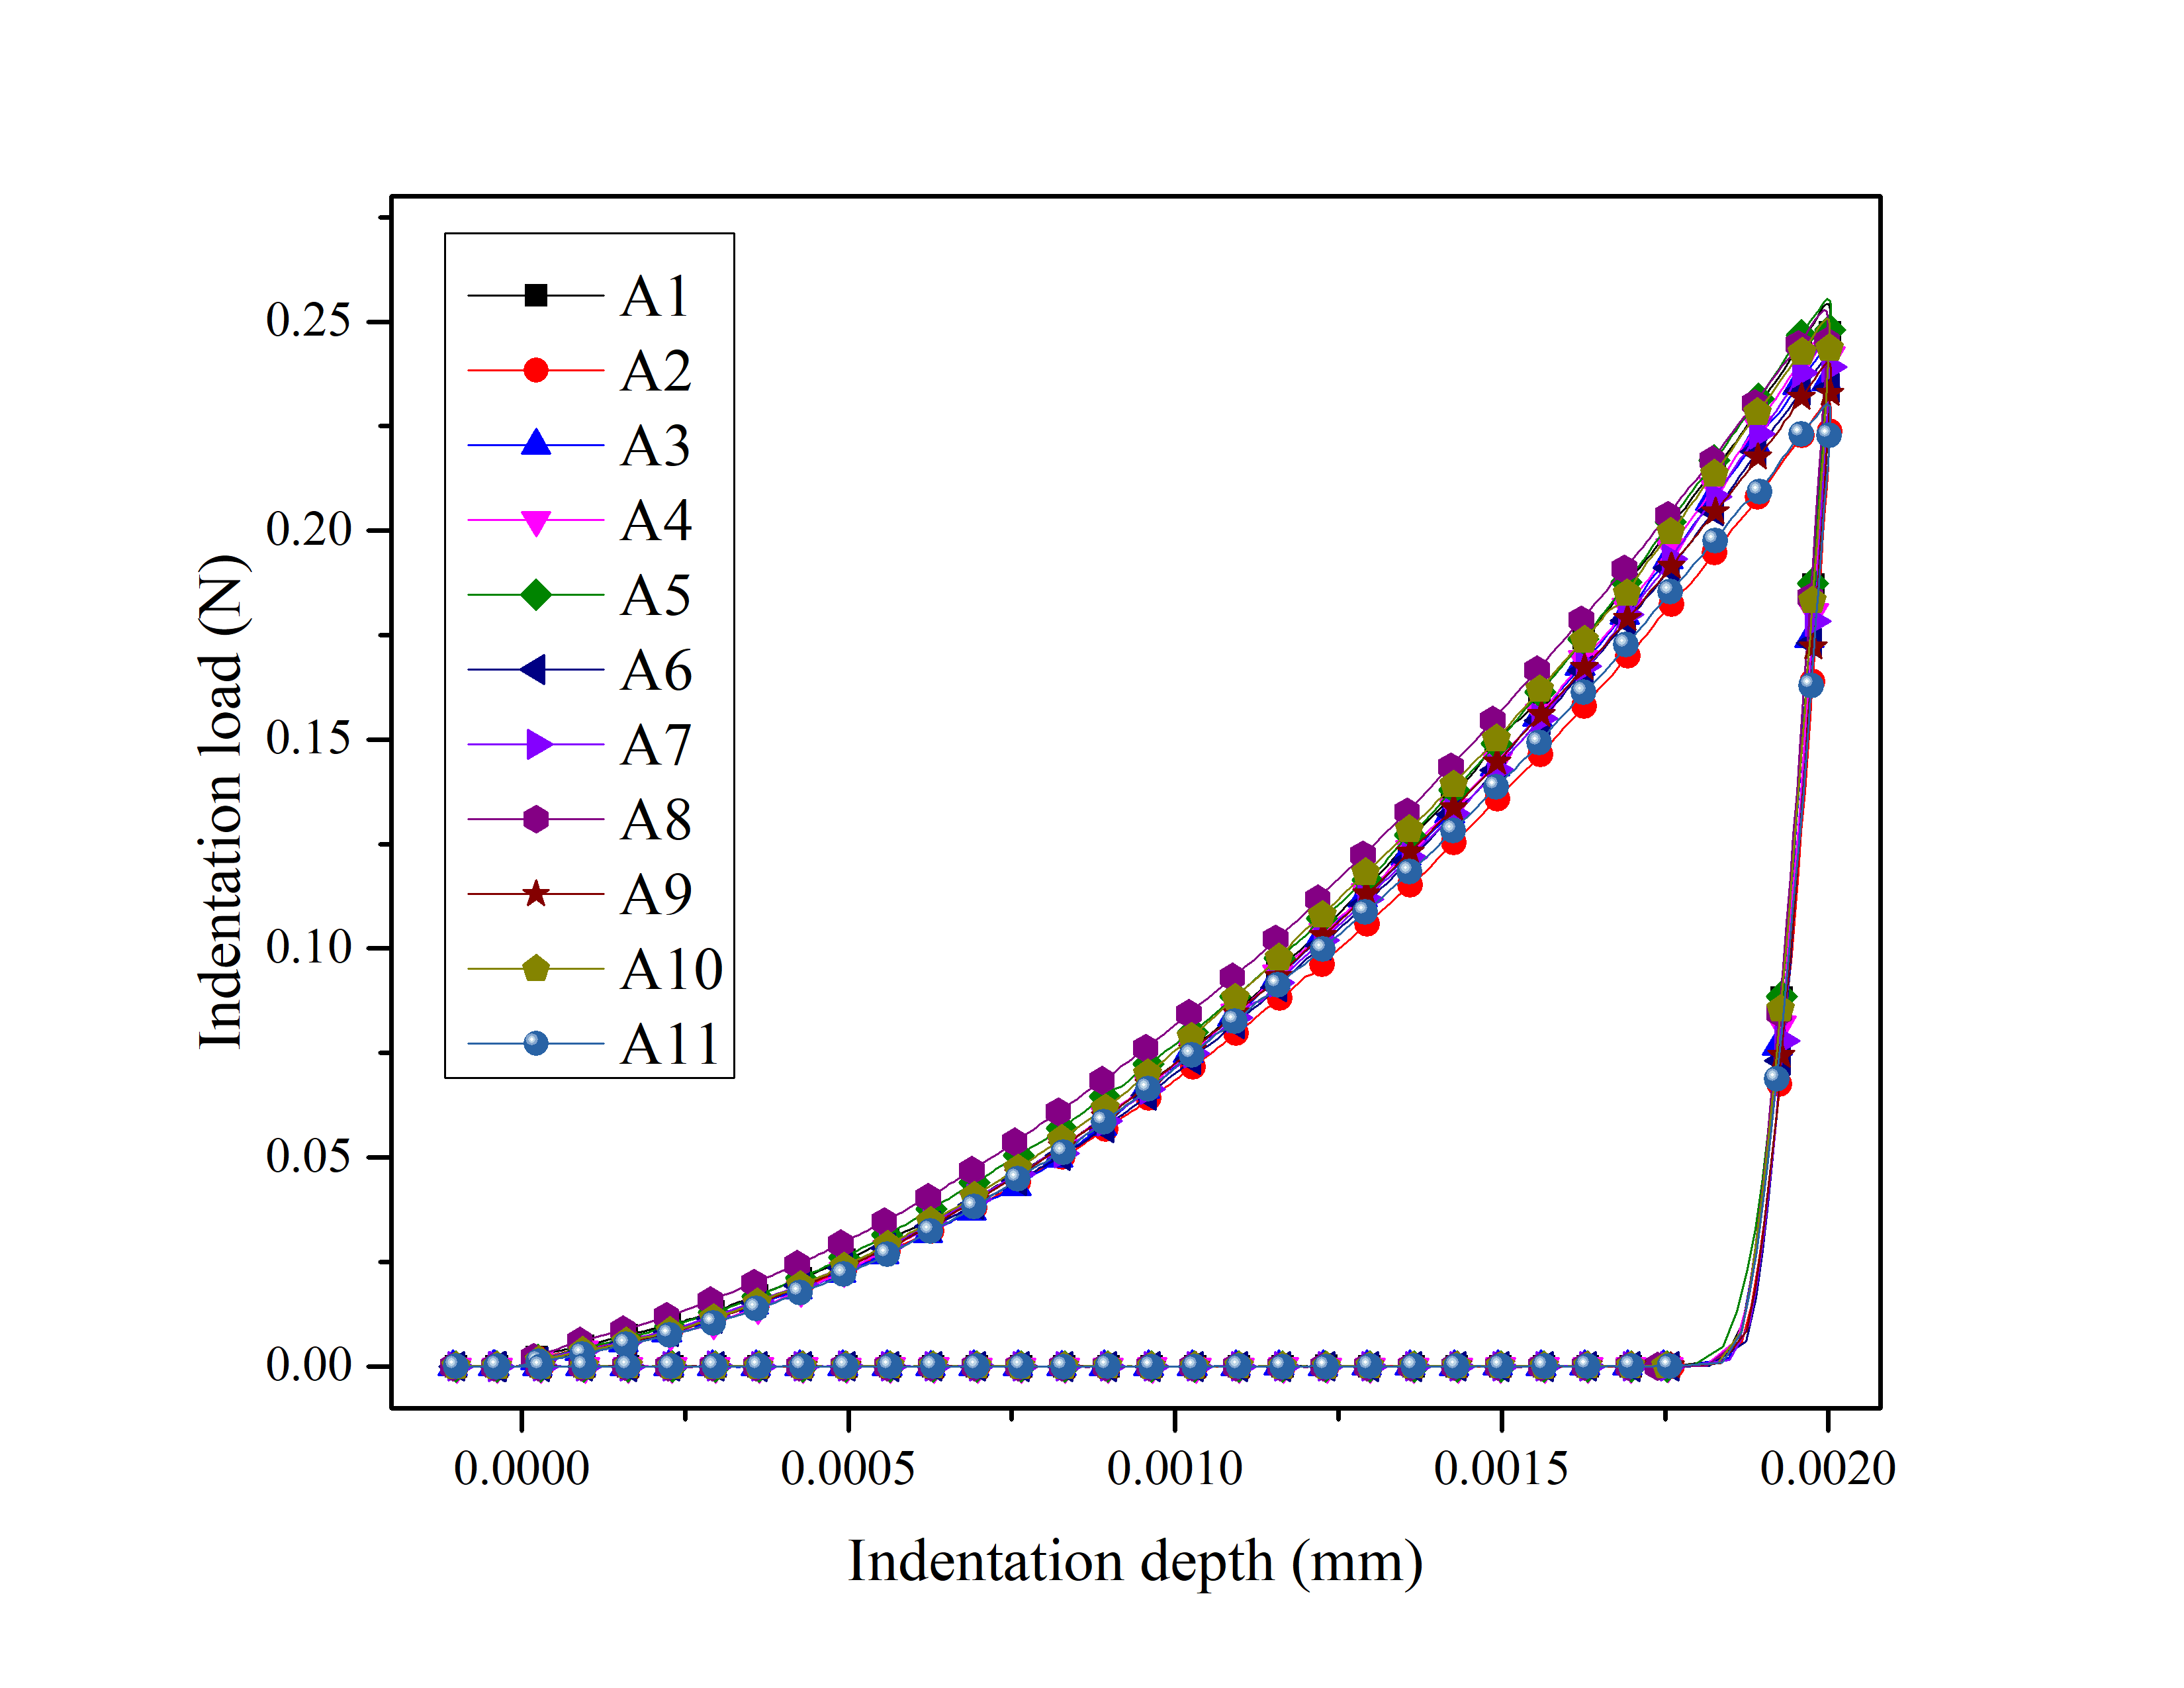
\includegraphics[width=0.5\textwidth]{./figs/P-hcurve_A.png}}
\subfloat[P-h curve of region B]{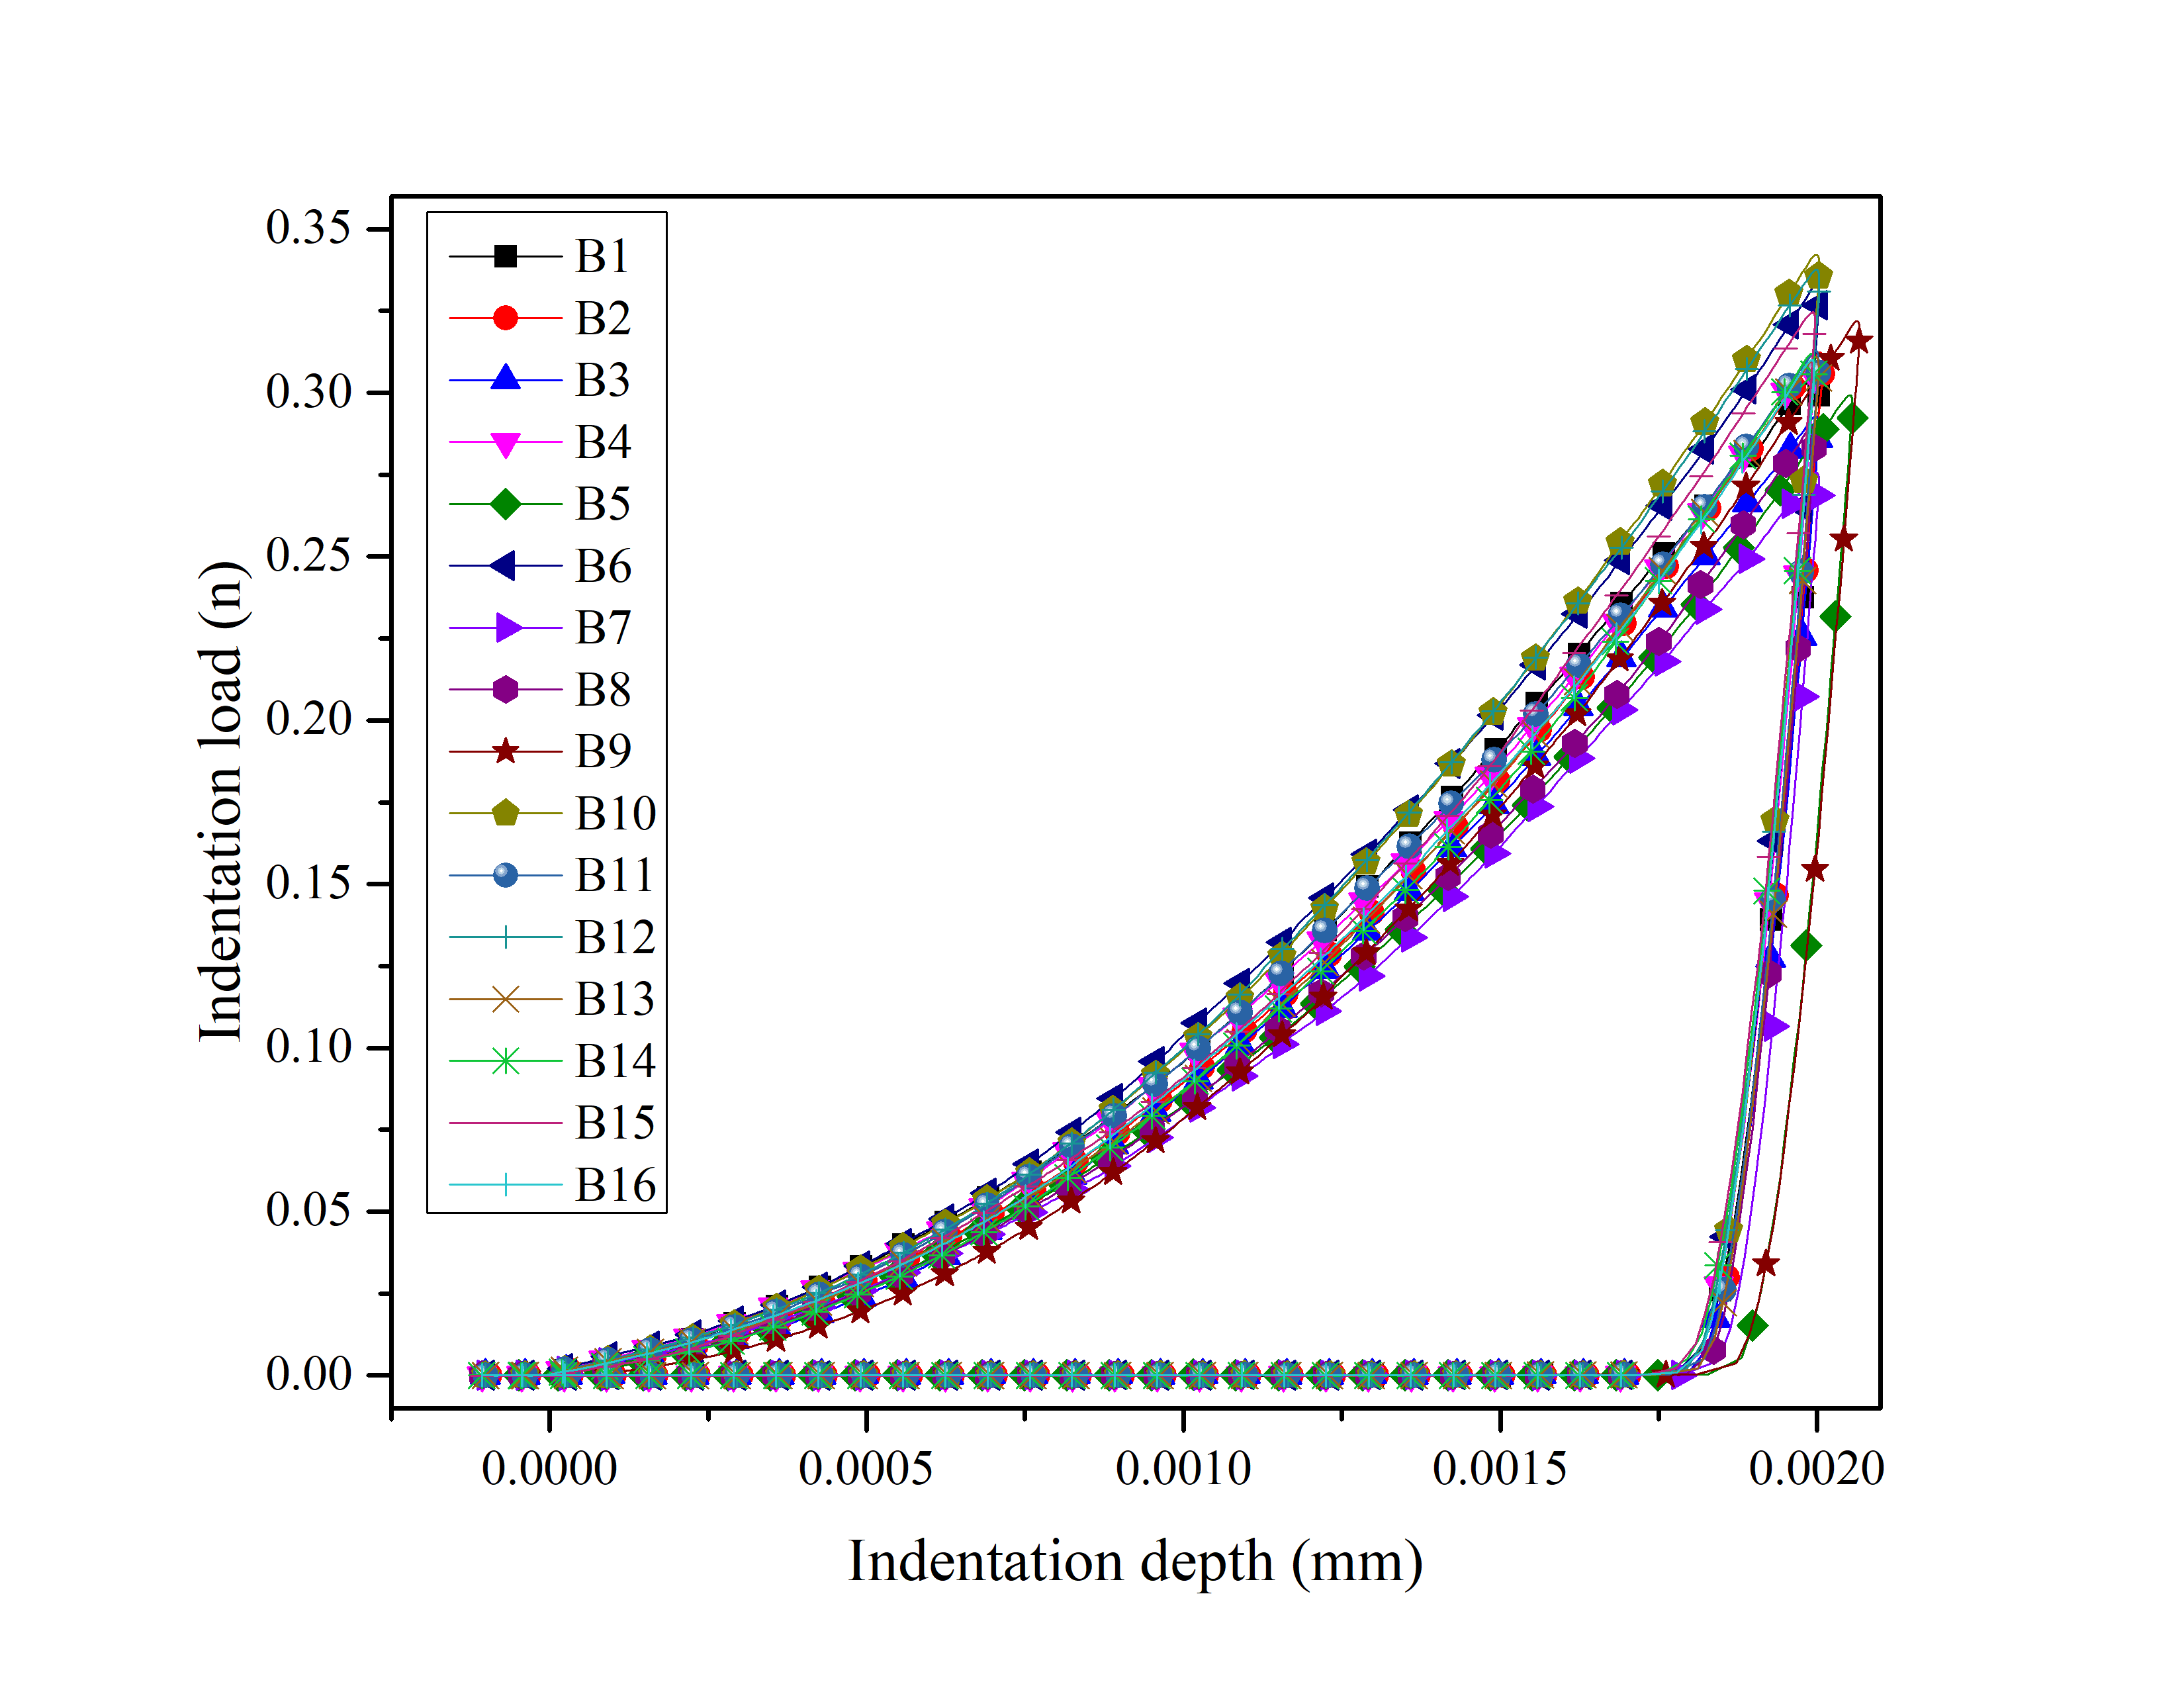
\includegraphics[width=0.5\textwidth]{./figs/P-hcurve_B.png}}

\subfloat[P-h curve of region C]{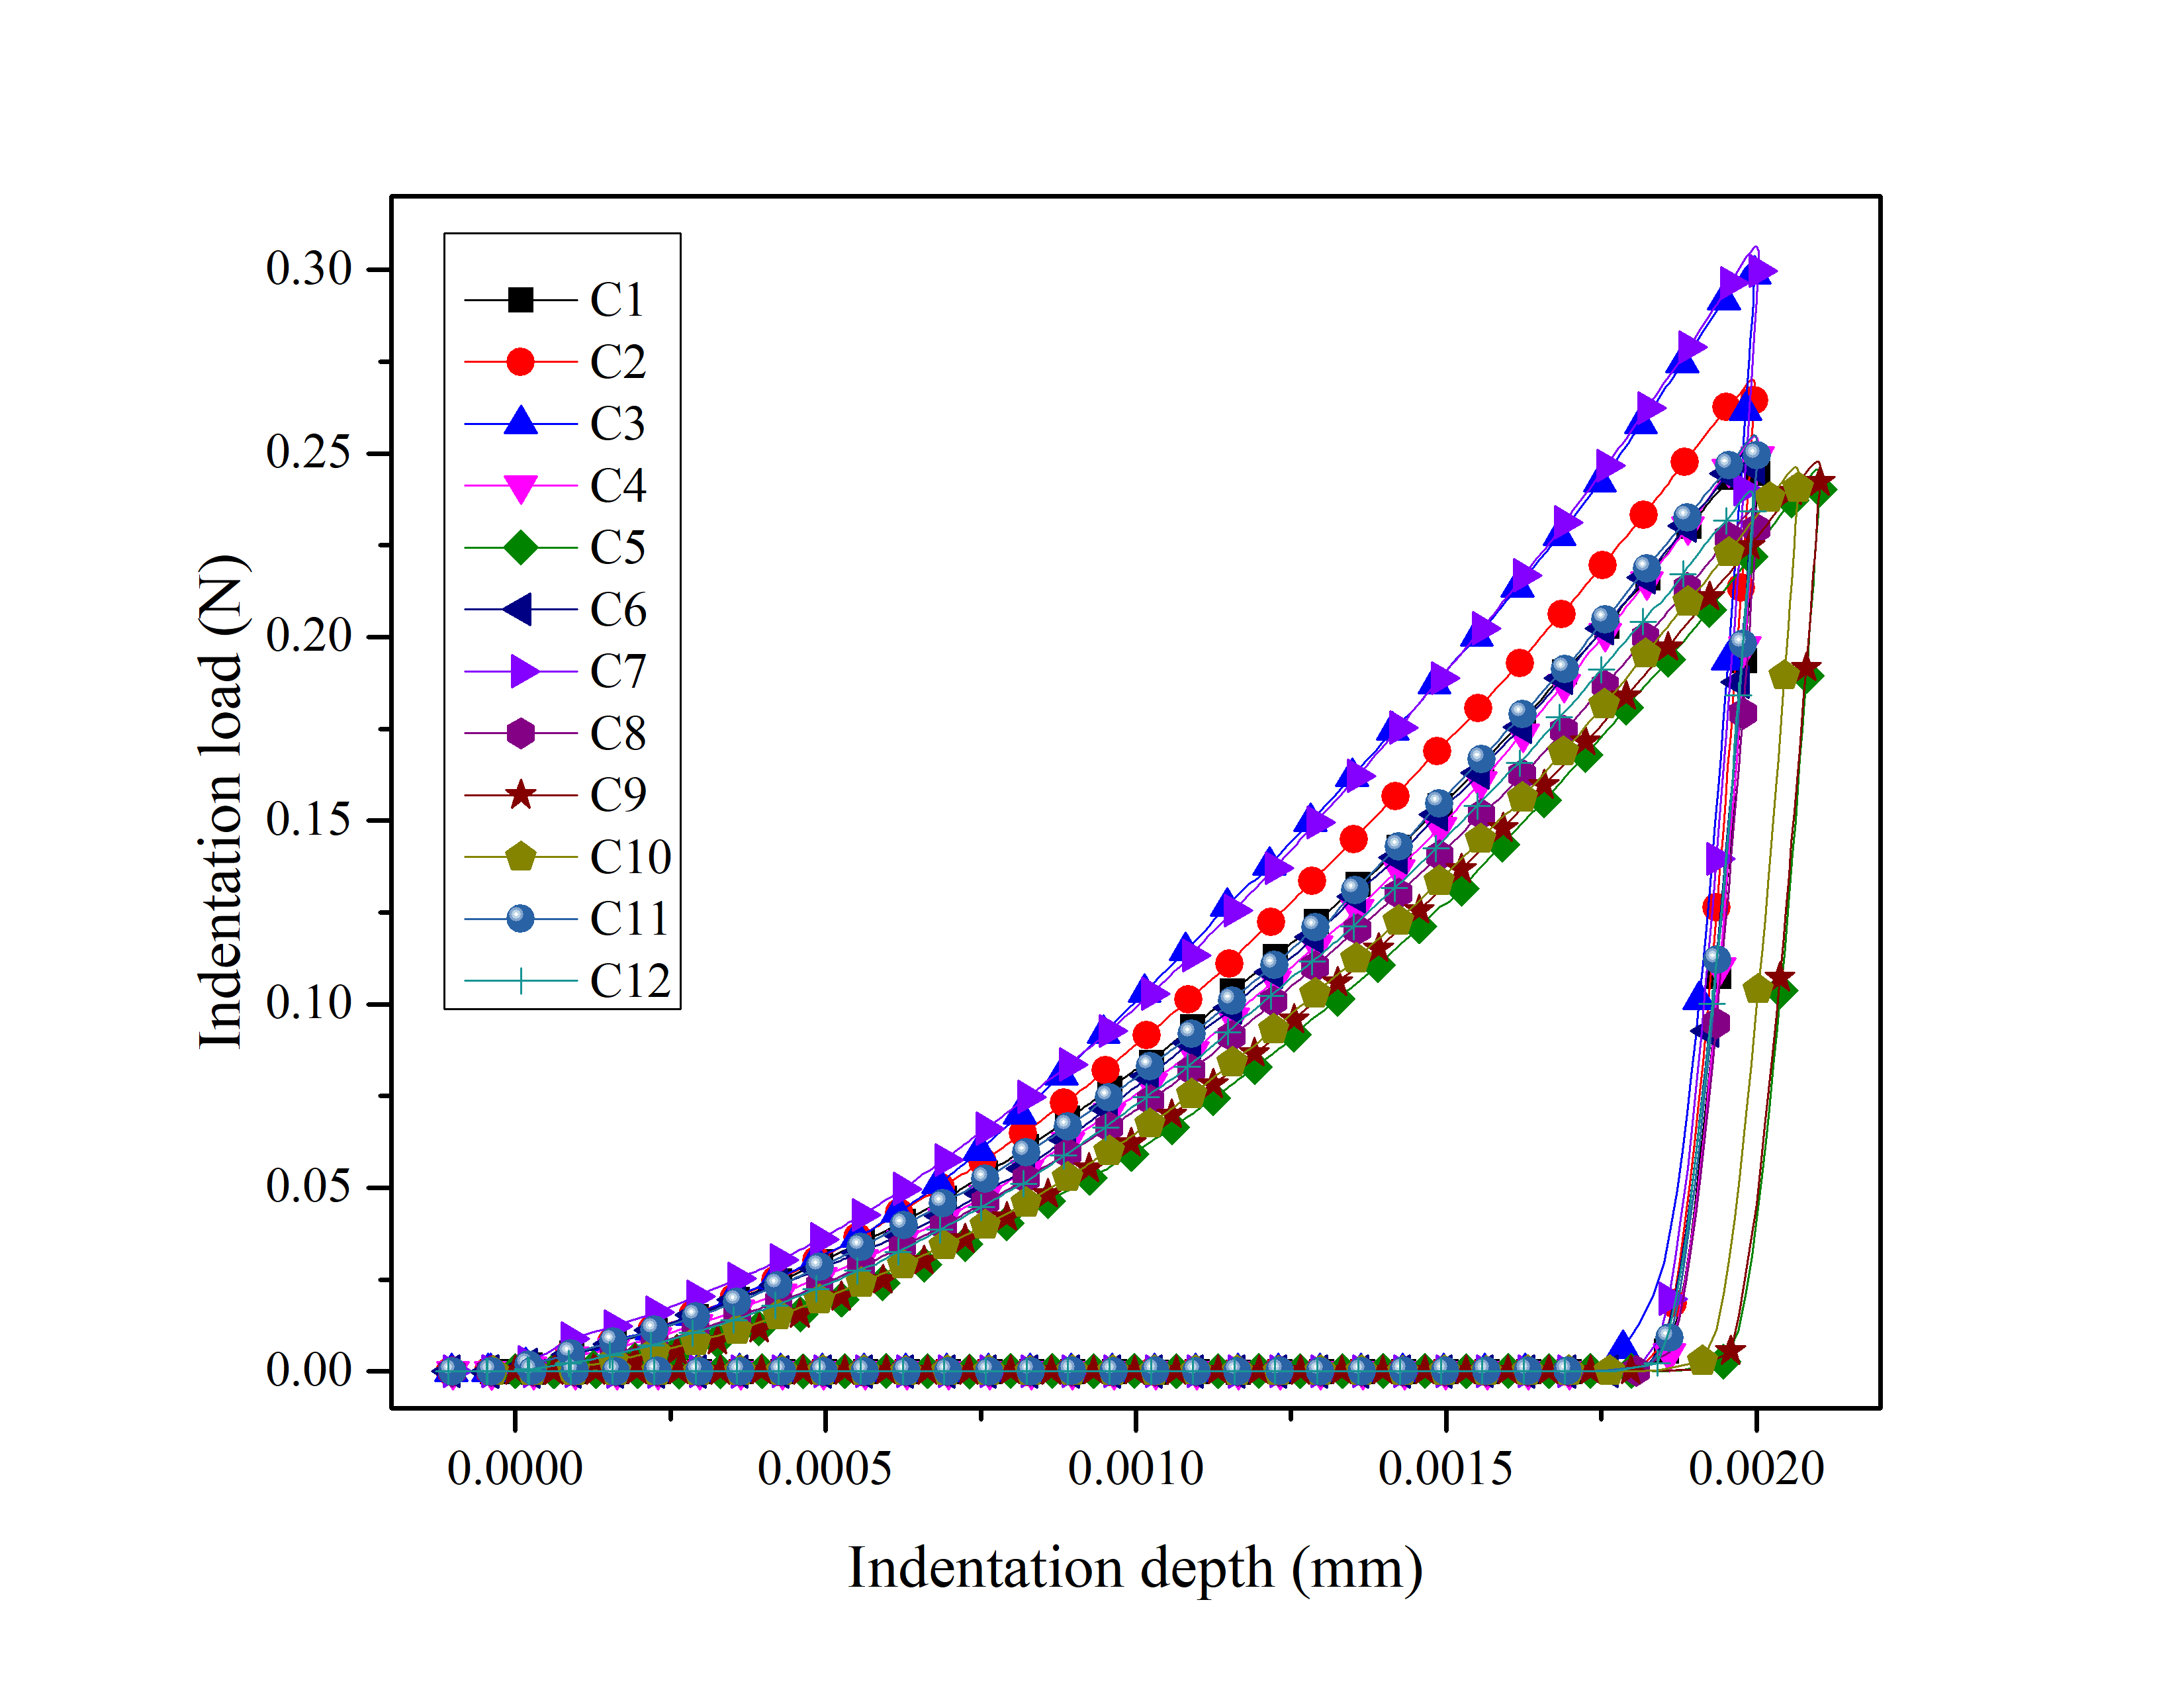
\includegraphics[width=0.5\textwidth]{./figs/P-hcurve_C.png}}
\subfloat[P-h curve of region C]{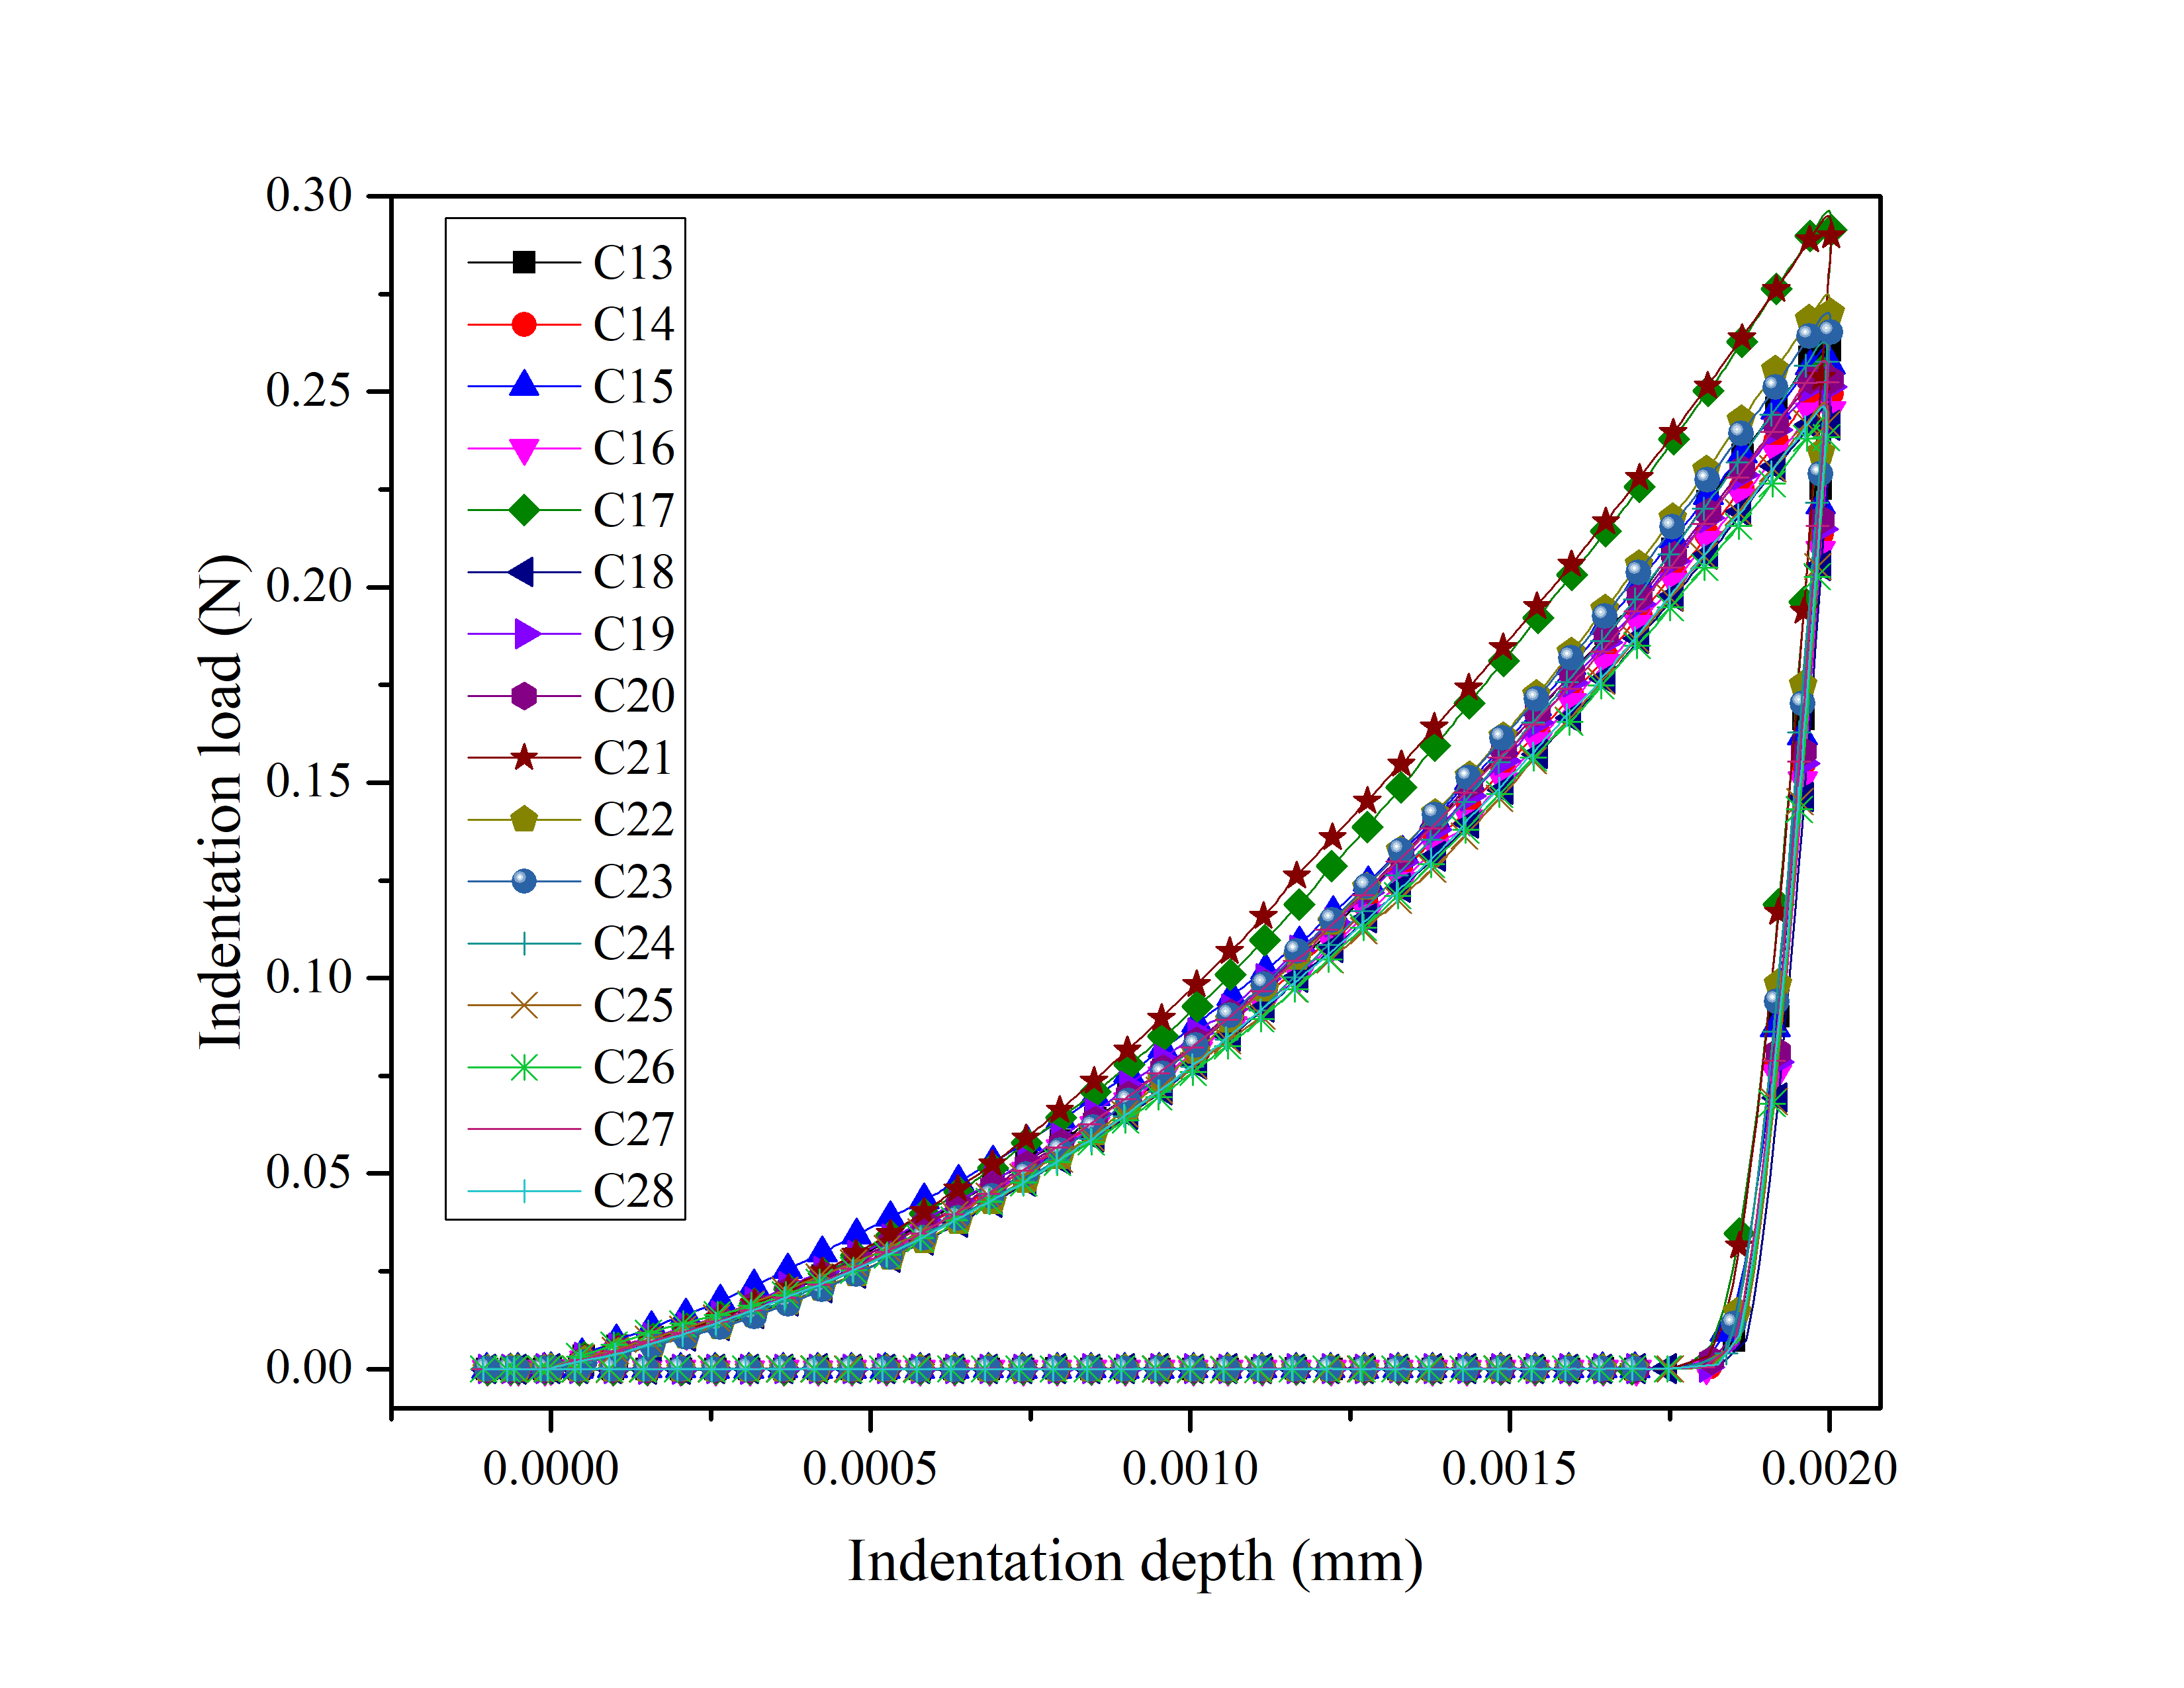
\includegraphics[width=0.5\textwidth]{./figs/P-hcurve_D.png}}

\subfloat[The mean of P-h curve]{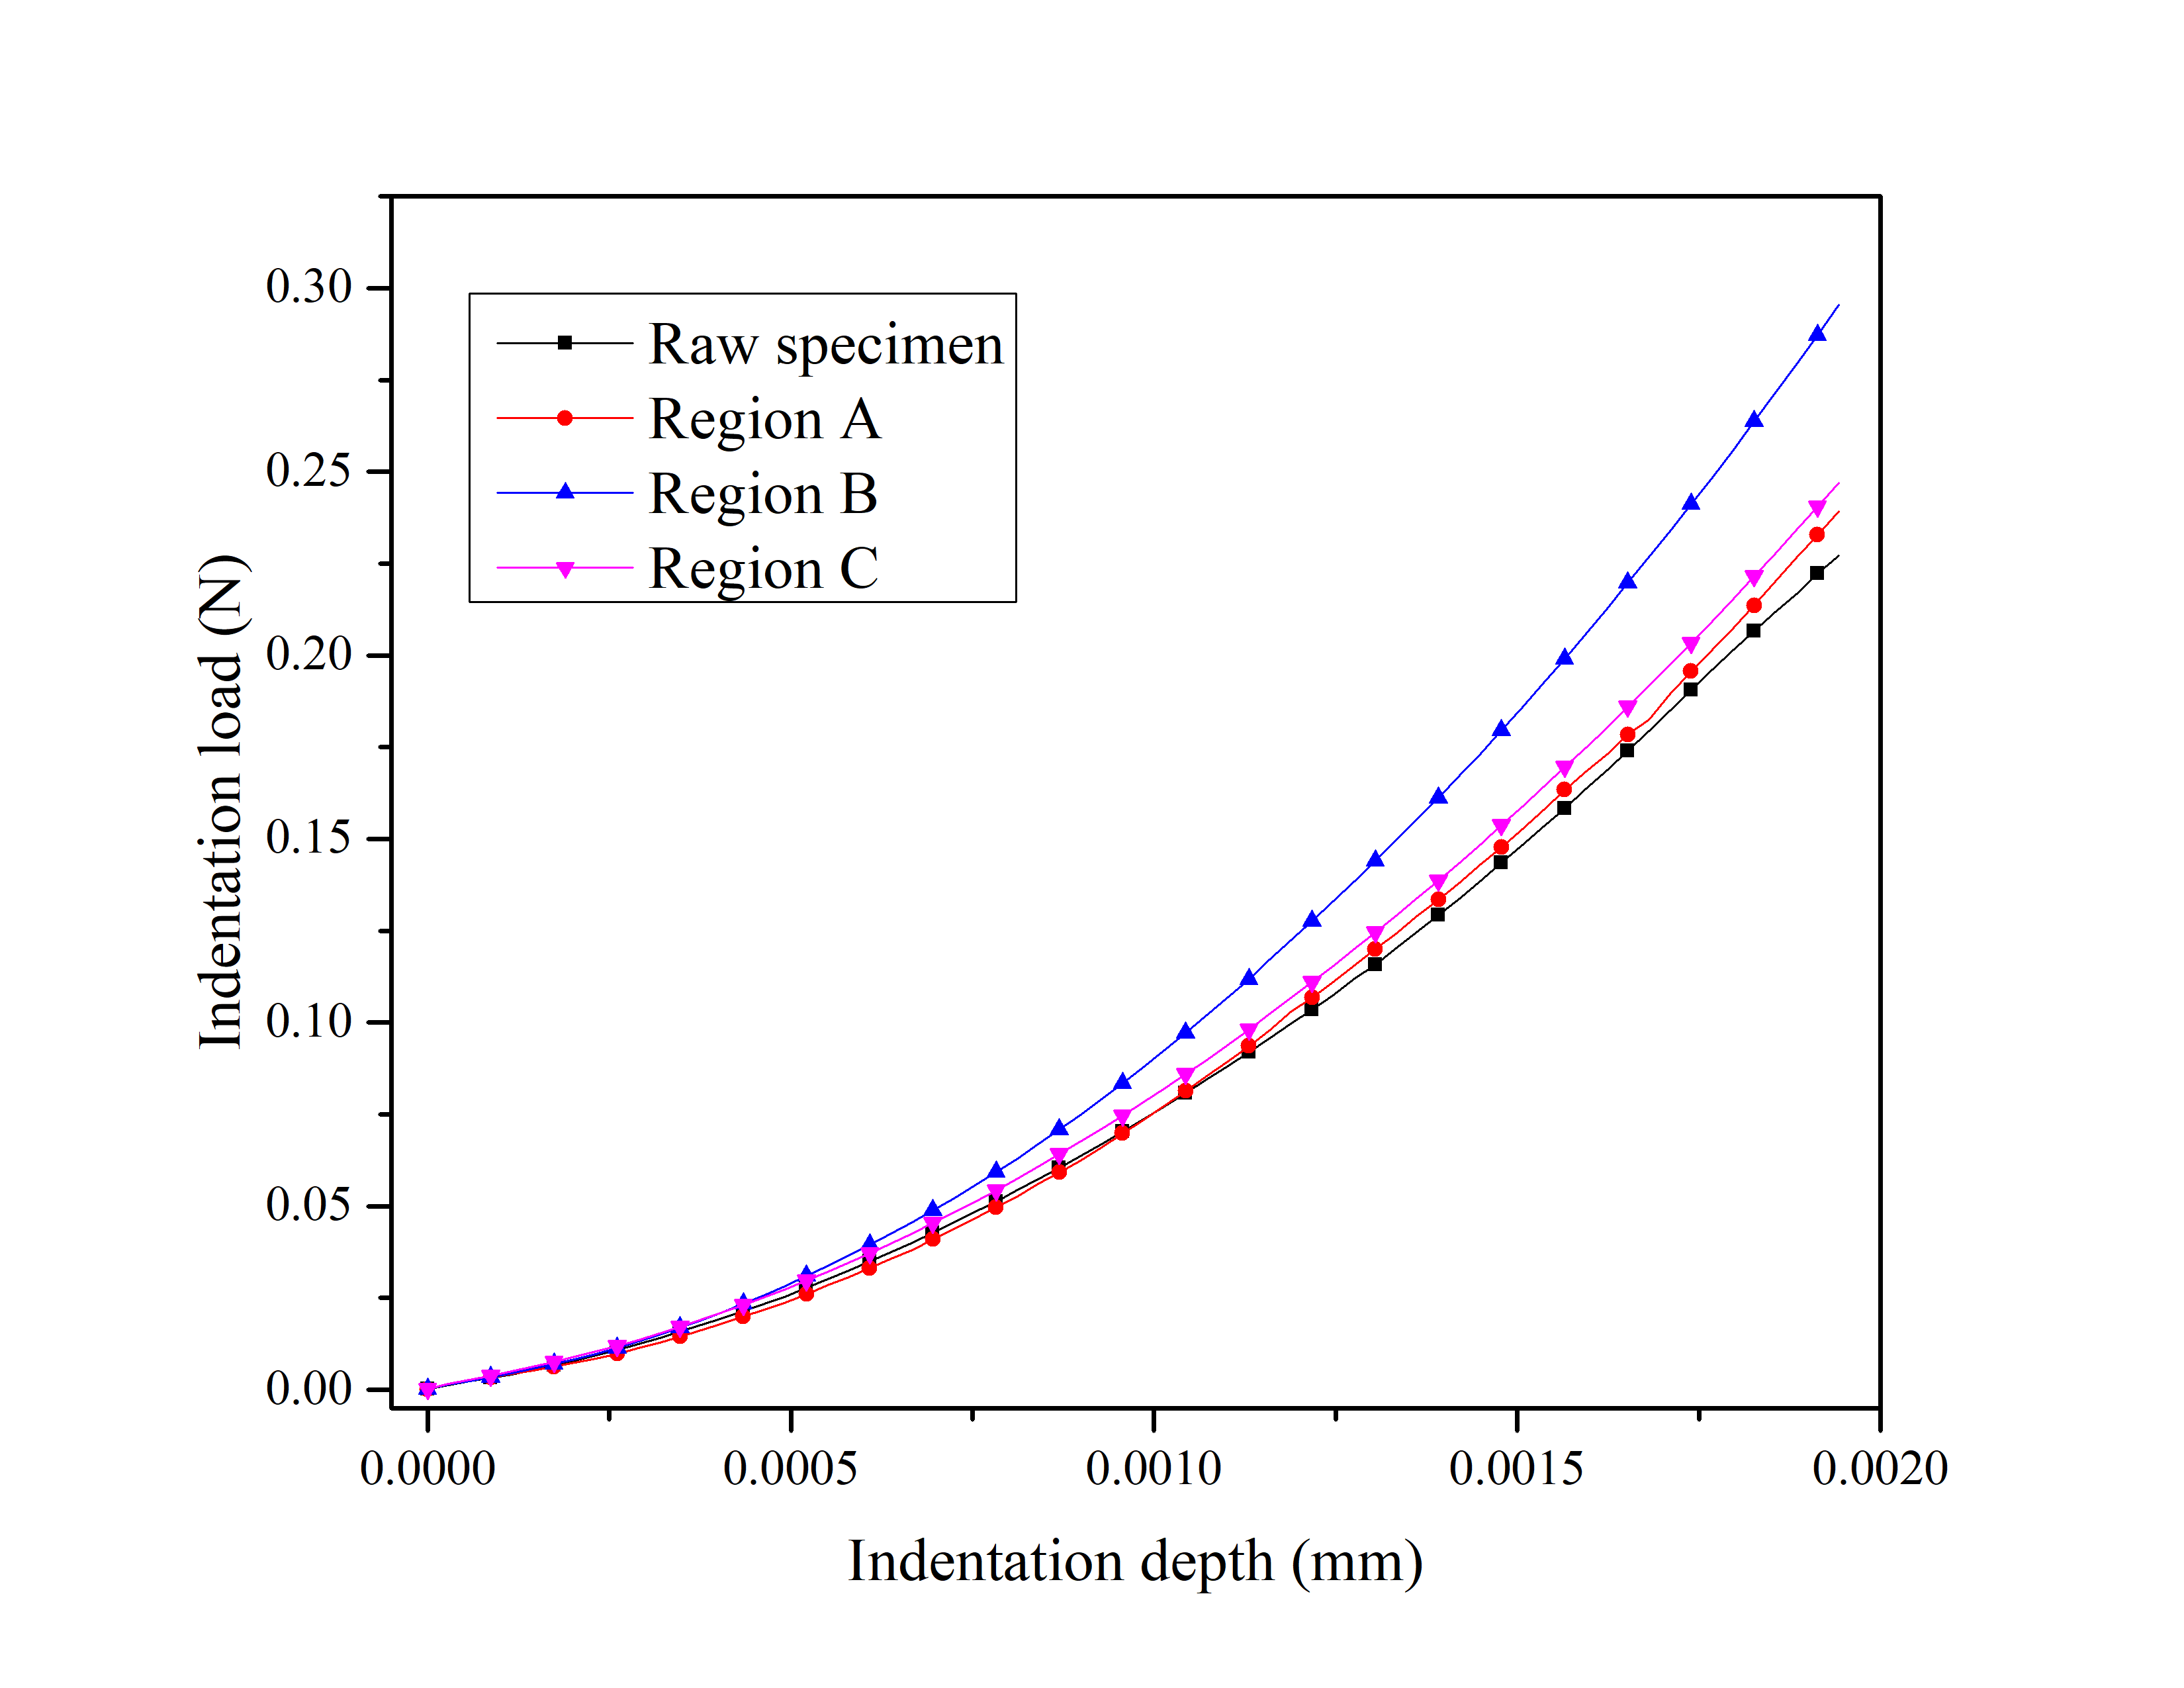
\includegraphics[width=0.5\textwidth]{./figs/meanoftest.png}}
\caption{The Indentation test results of of formed specimen}
\label{fig:phcurve region}
\end{figure}

\subsection{Results of inverse problem}

The number of snapshots is 100. In order to make the snapshots contain complete information of material parameters and P-h curves, a certain number of uniform samples is needed. The Latin hypercube design (LHD) \cite{iman2008latin} is good choice to generate the uniform samples in the material parameters' space. After that, the FE simulations are implemented to calculate the P-h curve of every material parameters sample. The P-h curves obtained from FE simulations are used to compose the response matrix $\mathbf{Y}$. Based on Eq.~\ref{eq:covariancematrix},\ref{eq:eigenequation},\ref{eq:PODbasis}, the basis vectors and eigenvalues can be calculated. According to the kinetic energy, the truncated basis $\bar{\mathbf{\Phi}}$ is determined. The coefficient vectors of snapshots are calculated by Eq.~\ref{eq:coefficient of POD}. Afterward, the connection between the material parameters and POD coefficient vectors is constructed with NN based on the snapshots and its coefficient vectors.

Before implementing the proposed method to identify the material properties, the accuracy of POD and NN need to be tested. In this study, the number of test samples is 20 and generated by the same way of snapshots. The $R^2$ is calculated with 0.983. The FE response and the results of proposed method are presented in Fig.\ref{fig:accuracy_of_NN}. It can be shown that NN and POD is accurate enough to implement the proposed method.

\begin{figure}[h!]
\centering
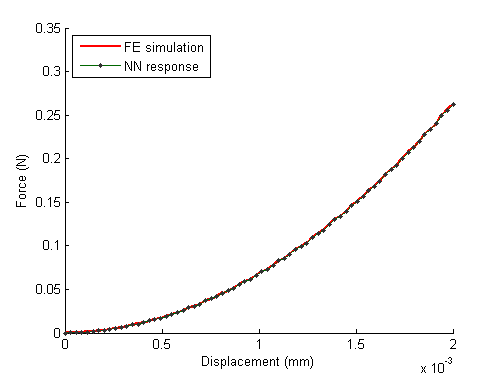
\includegraphics[width=0.6\textwidth]{./figs/accuracy_of_NN.png}
\caption{The responses of FE and proposed method}
\label{fig:accuracy_of_NN}
\end{figure}

The prior distribution is supposed to be Gaussian for all observations. Its means are from \cite{vedantam2006johnson} in which the A, B and n of DP590 are $430MPa$, $824MPa$ and $0.510$, respectively. Its standard deviations are supposed as 10\% of the means. This is a very wide distribution and denotes that the effect from priors on the posteriors is small.

The coefficient vector of observations is determined by least square fit or weighted residuals. Then with the well-constructed NN, the ABC-NPMC is used to calculate the approximate posteriors of material parameters. The posteriori material parameters of the raw specimen are presented in Fig.~\ref{fig:posterior DP}. The P-h curves calculated by mean of posteriori material parameters and the means of measurements of the raw specimen without formed are presented in Fig.~\ref{fig:comparison regions}.

\begin{figure}[h!]
\centering
\subfloat[Posterior of $\mathbf{A}$]{
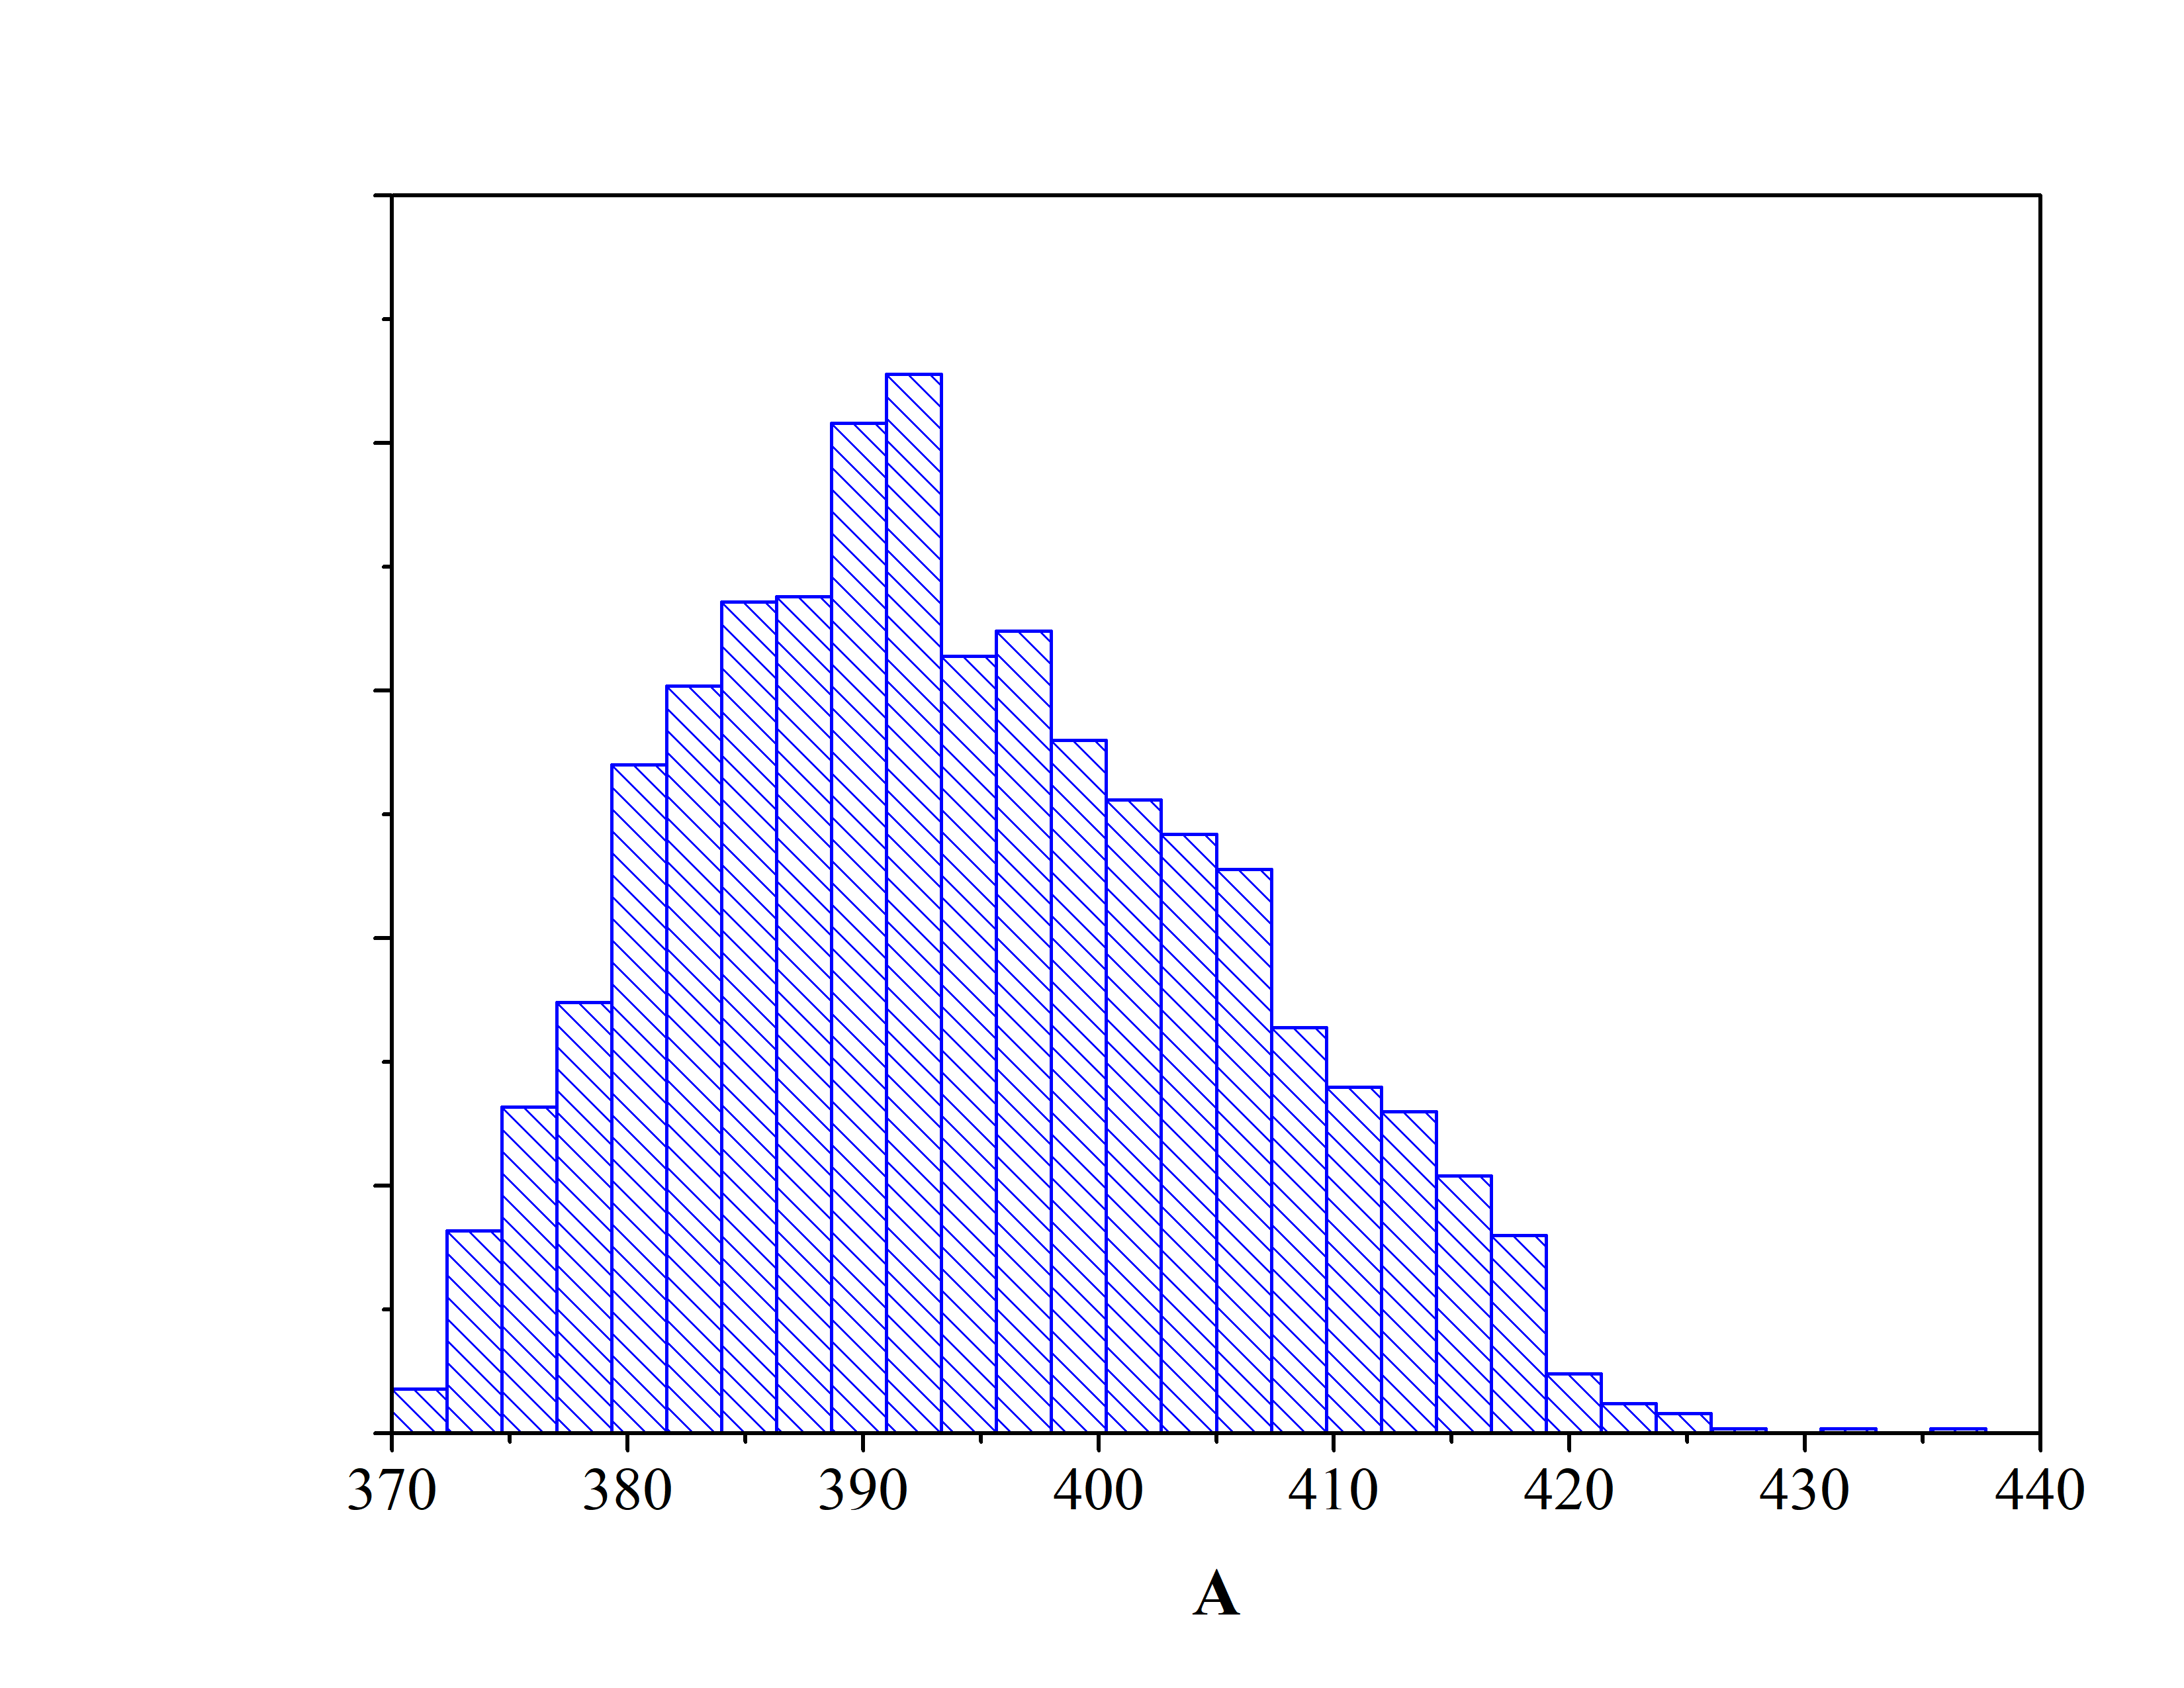
\includegraphics[width=0.3\textwidth]{./figs/posterior_DP_A.png}}
\subfloat[Posterior of $\mathbf{B}$]{
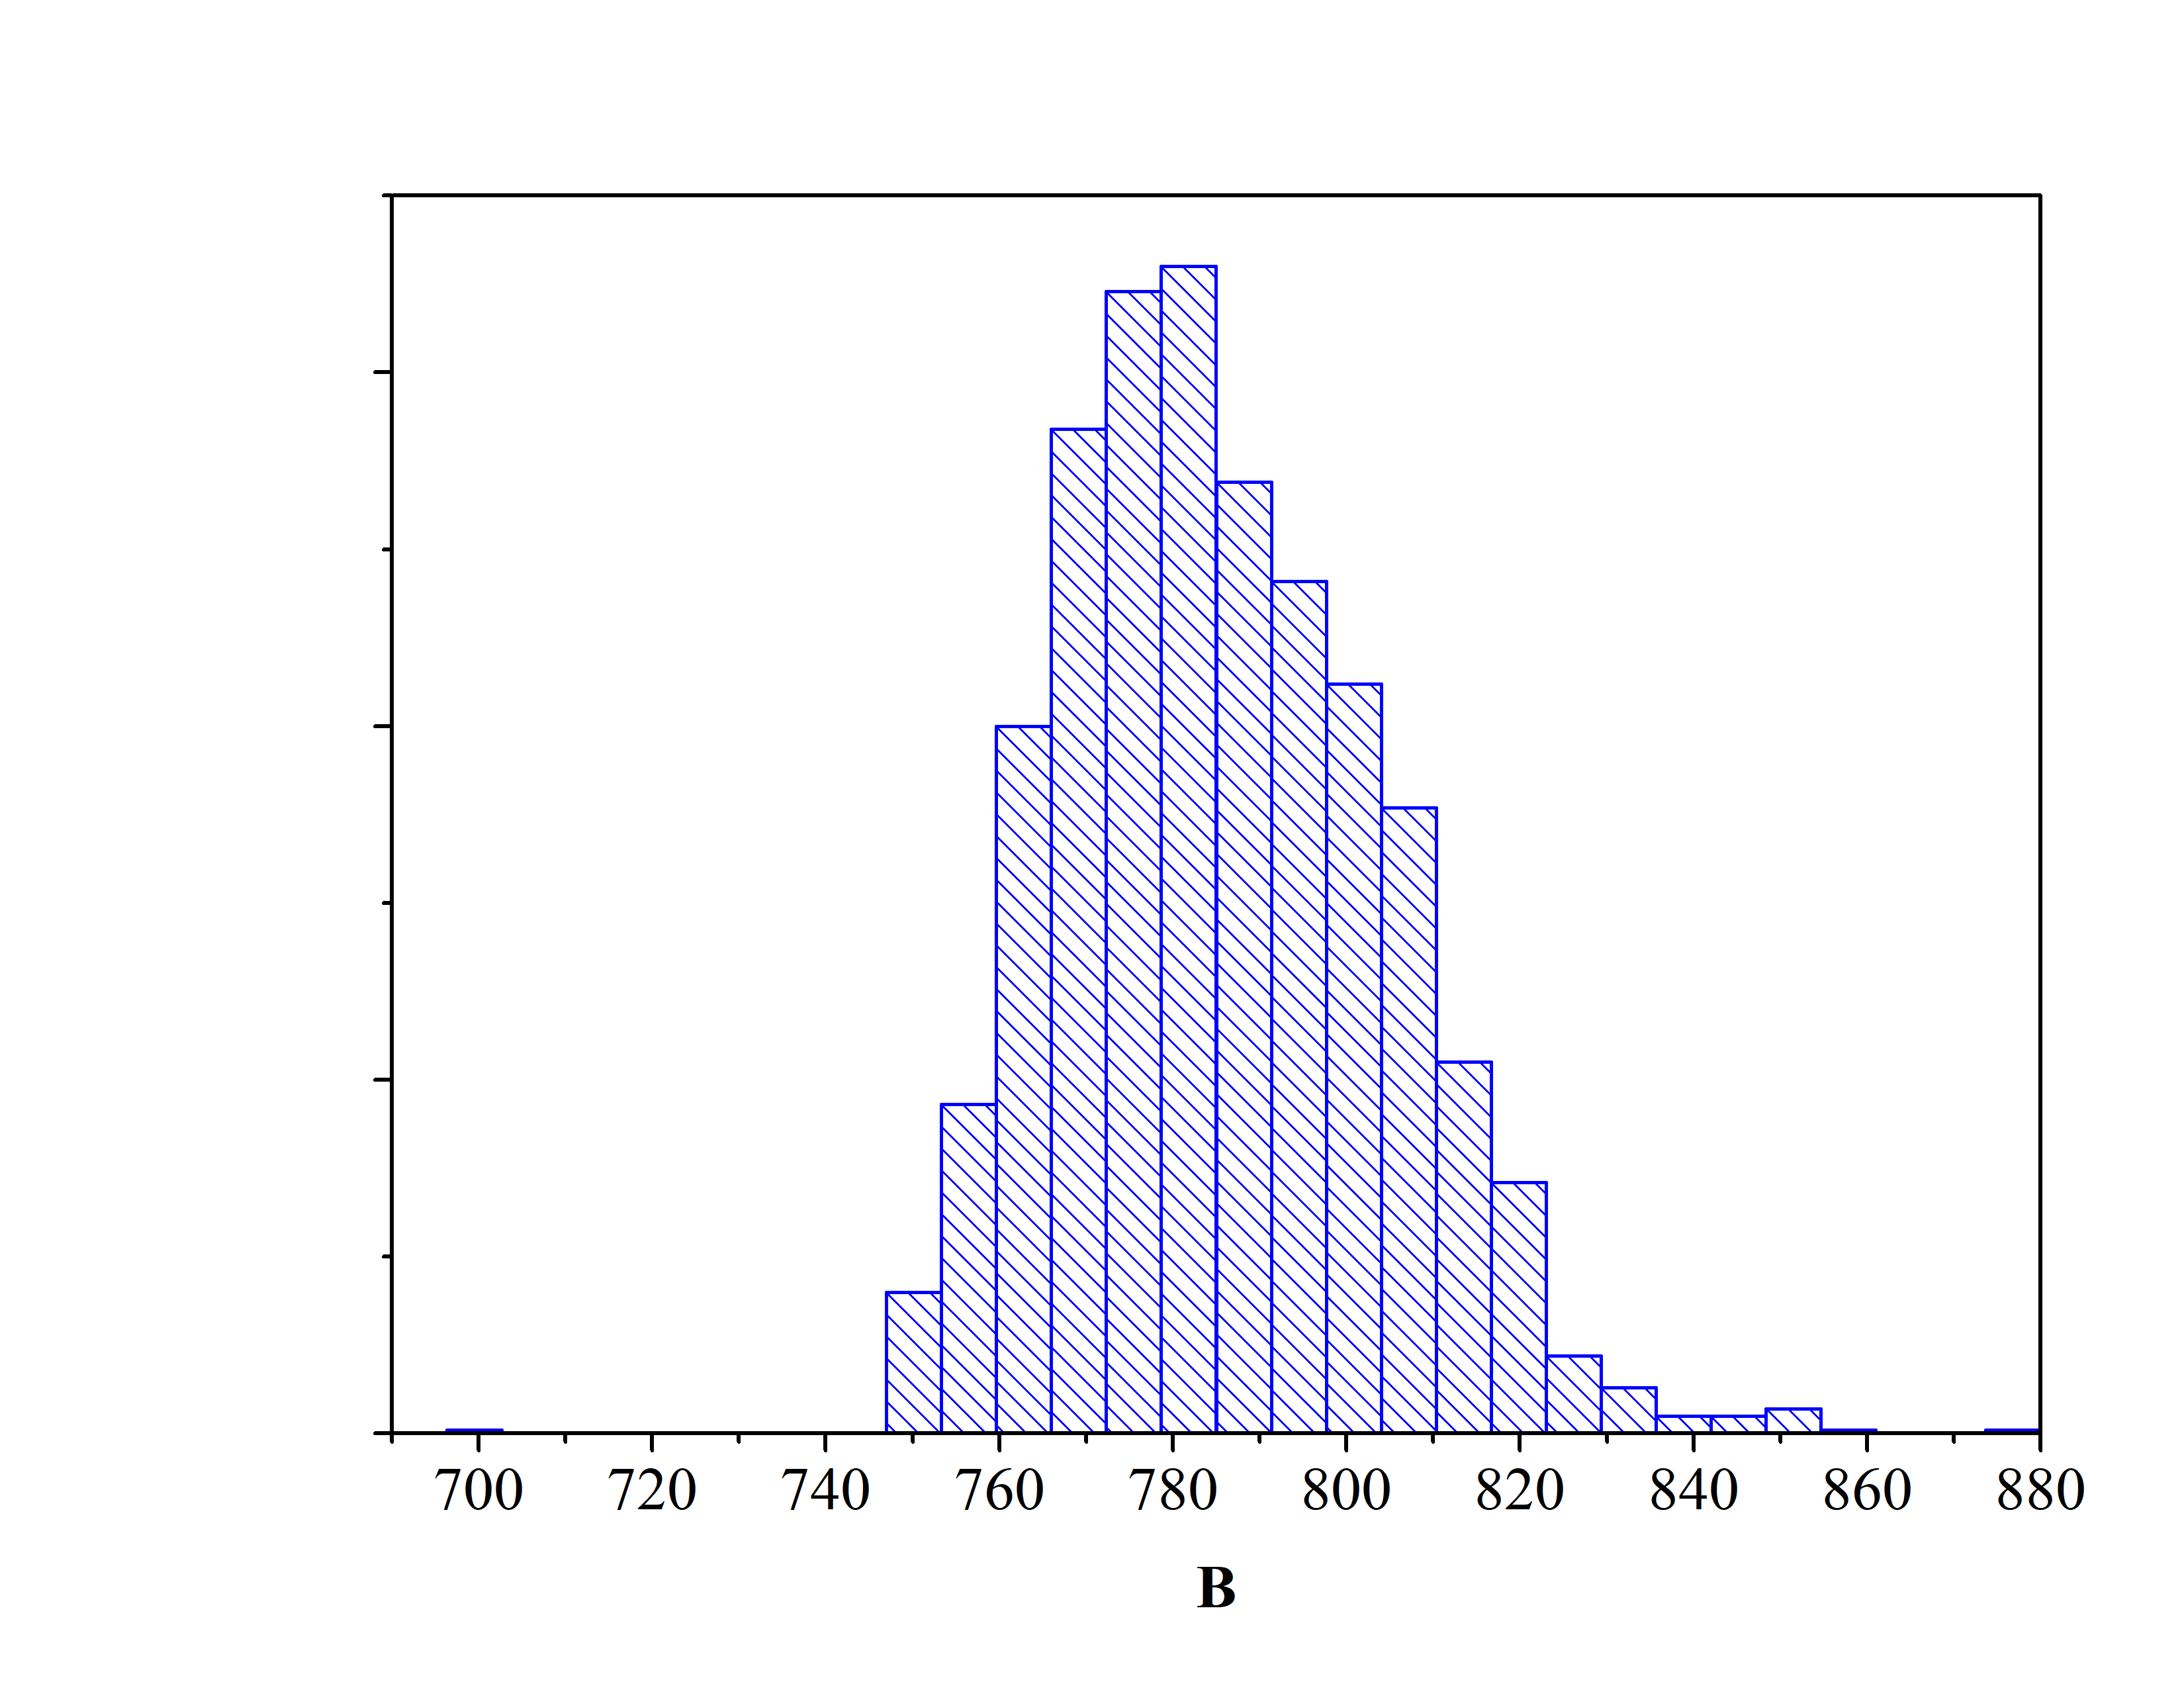
\includegraphics[width=0.3\textwidth]{./figs/posterior_DP_B.png}}
\subfloat[Posterior of $\mathbf{n}$]{
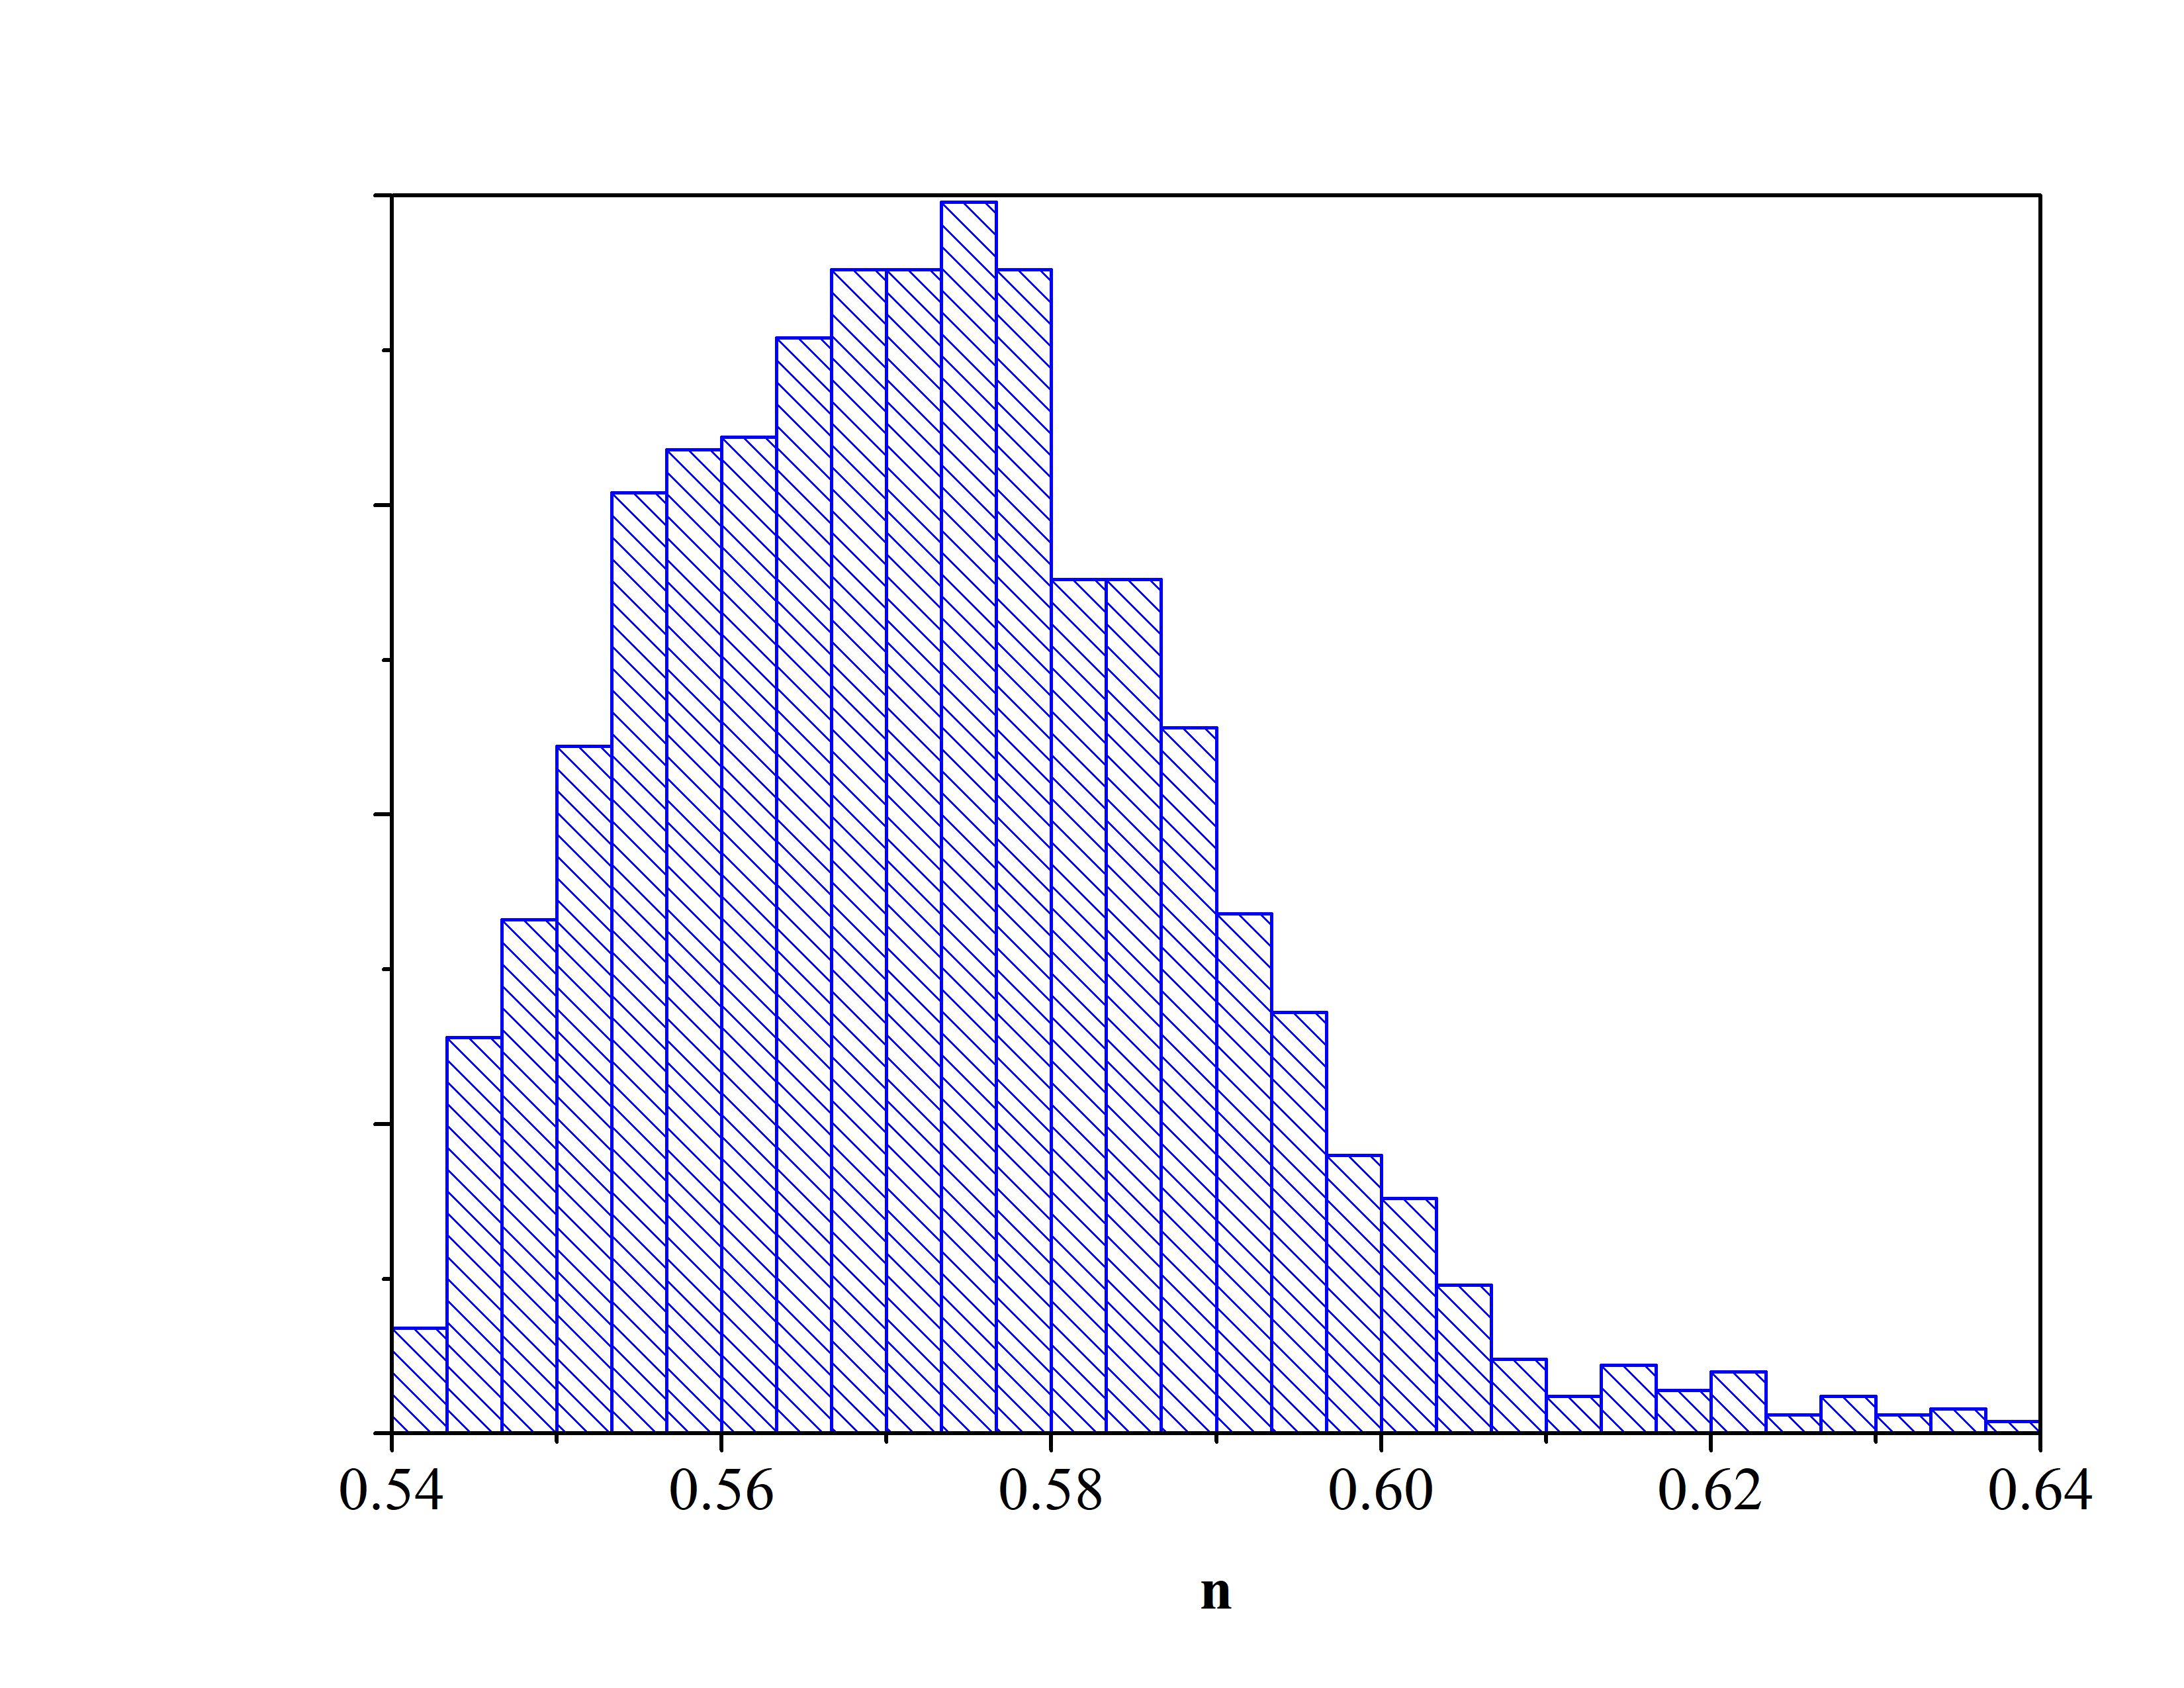
\includegraphics[width=0.3\textwidth]{./figs/posterior_DP_n.png}}
\caption{Posteriors of the specimen without formed}
\label{fig:posterior DP}
\end{figure}

The posteriori material parameters in region A, B and C regions are presented in Fig.~\ref{fig:posterior formed}. The P-h curves calculated by the means of posteriori material parameters and the means of measurement in region A, B and C are presented in Fig.~\ref{fig:comparison regions}. From Fig.\ref{fig:comparison regions}, it shows that the prediction of proposed methods can match the measurements of indentation test very well. From  Fig.\ref{fig:posterior DP}, \ref{fig:posterior formed} and the standard deviation in Table.\ref{table:results}, it shows the proposed method can obtain a distribution of the posteriori parameters which is very useful for uncertainty quantification or reliability analysis.

\begin{table}[h!]
\centering
\caption{The means and standard deviation of posteriors}
\begin{tabular}{c c c c c c c} 
 \hline
  & \multicolumn{3}{c}{Means} & \multicolumn{3}{c}{Standard deviations} \\
 \cline{2-7}
  & $\mathbf{A}$ & $\mathbf{B}$ & $\mathbf{n}$ & $\mathbf{A}$ & $\mathbf{B}$ & $\mathbf{n}$\\
  \hline
 Raw specimen & 387.1 & 785.6 & 0.57 & 11.23 & 18.27 & 0.0163\\
 Region A & 400.4 & 795.4 & 0.5452 & 16.26 & 24.53 & 0.0184\\
 Region B & 525.1 & 843.9 & 0.4352 & 12.47 & 23.57 & 0.0185\\
 Region C & 430.6 & 798.9 & 0.5283 & 14.76 & 22.90 & 0.0166\\
 \hline
\end{tabular}
\label{table:results}
\end{table}

\begin{figure}[h!]
\centering
\subfloat[Posterior of $\mathbf{A}$]{
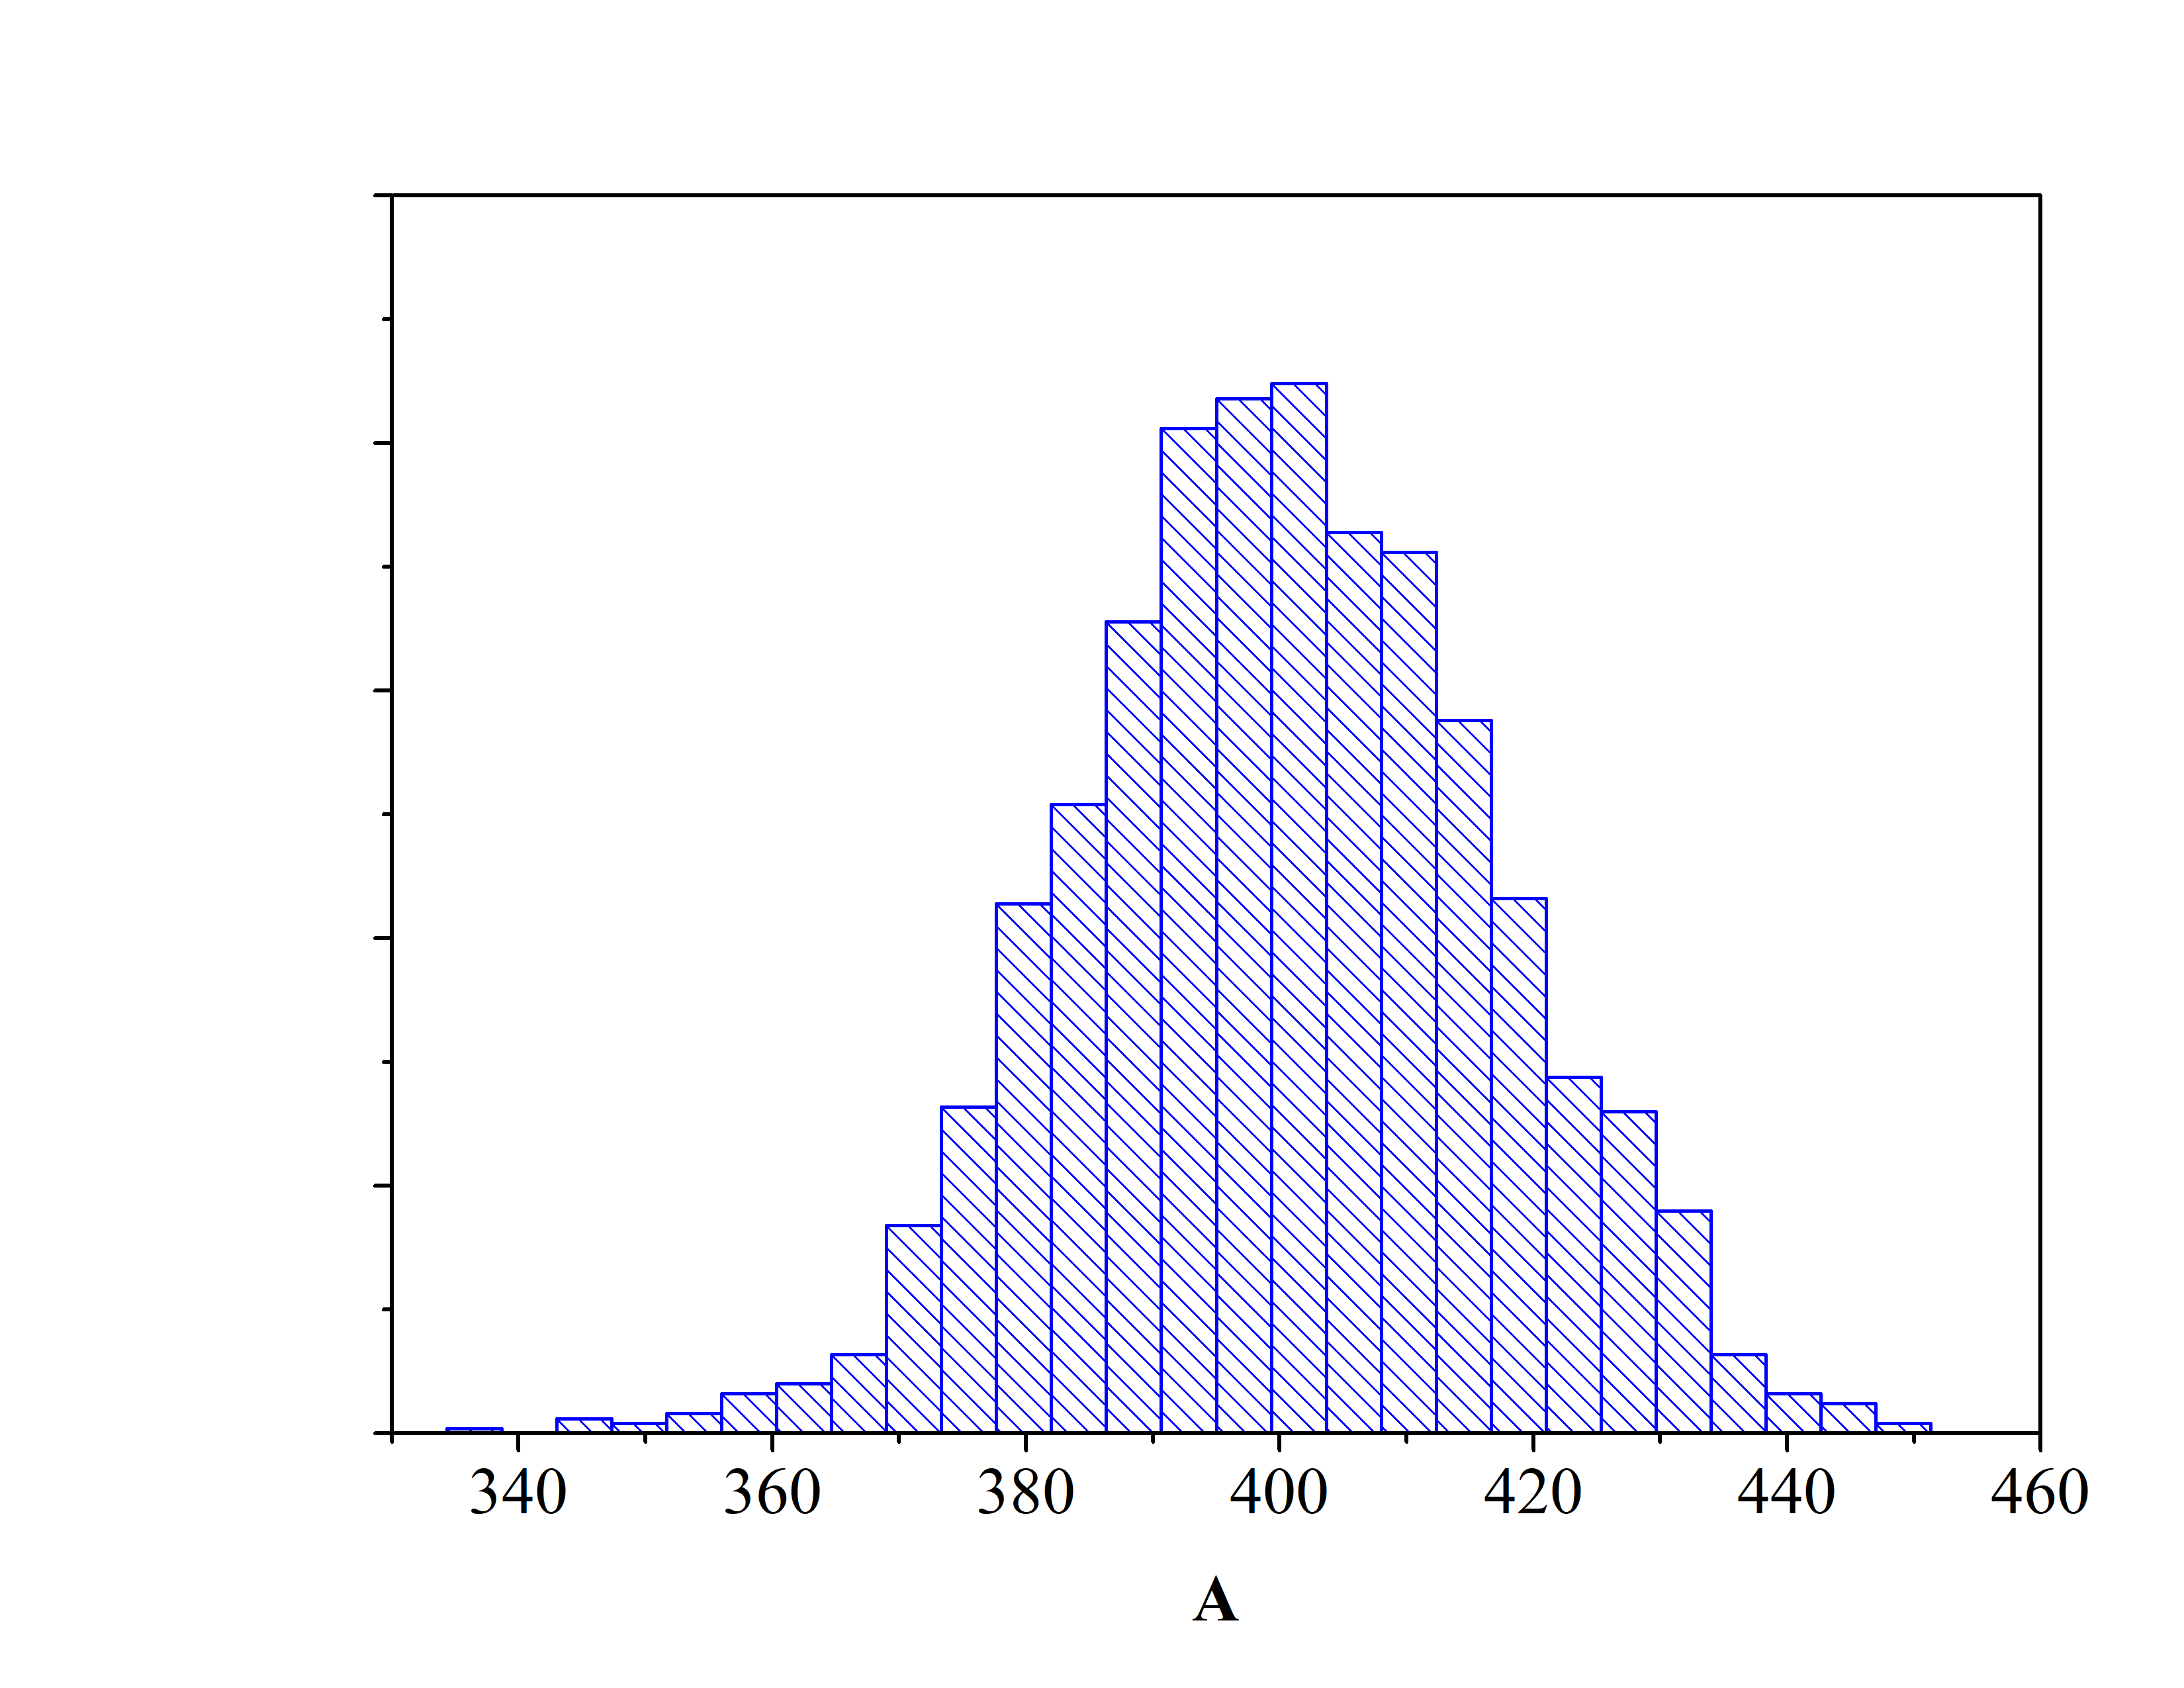
\includegraphics[width=0.3\textwidth]{./figs/posterior_A_A.png}}
\subfloat[Posterior of $\mathbf{B}$]{
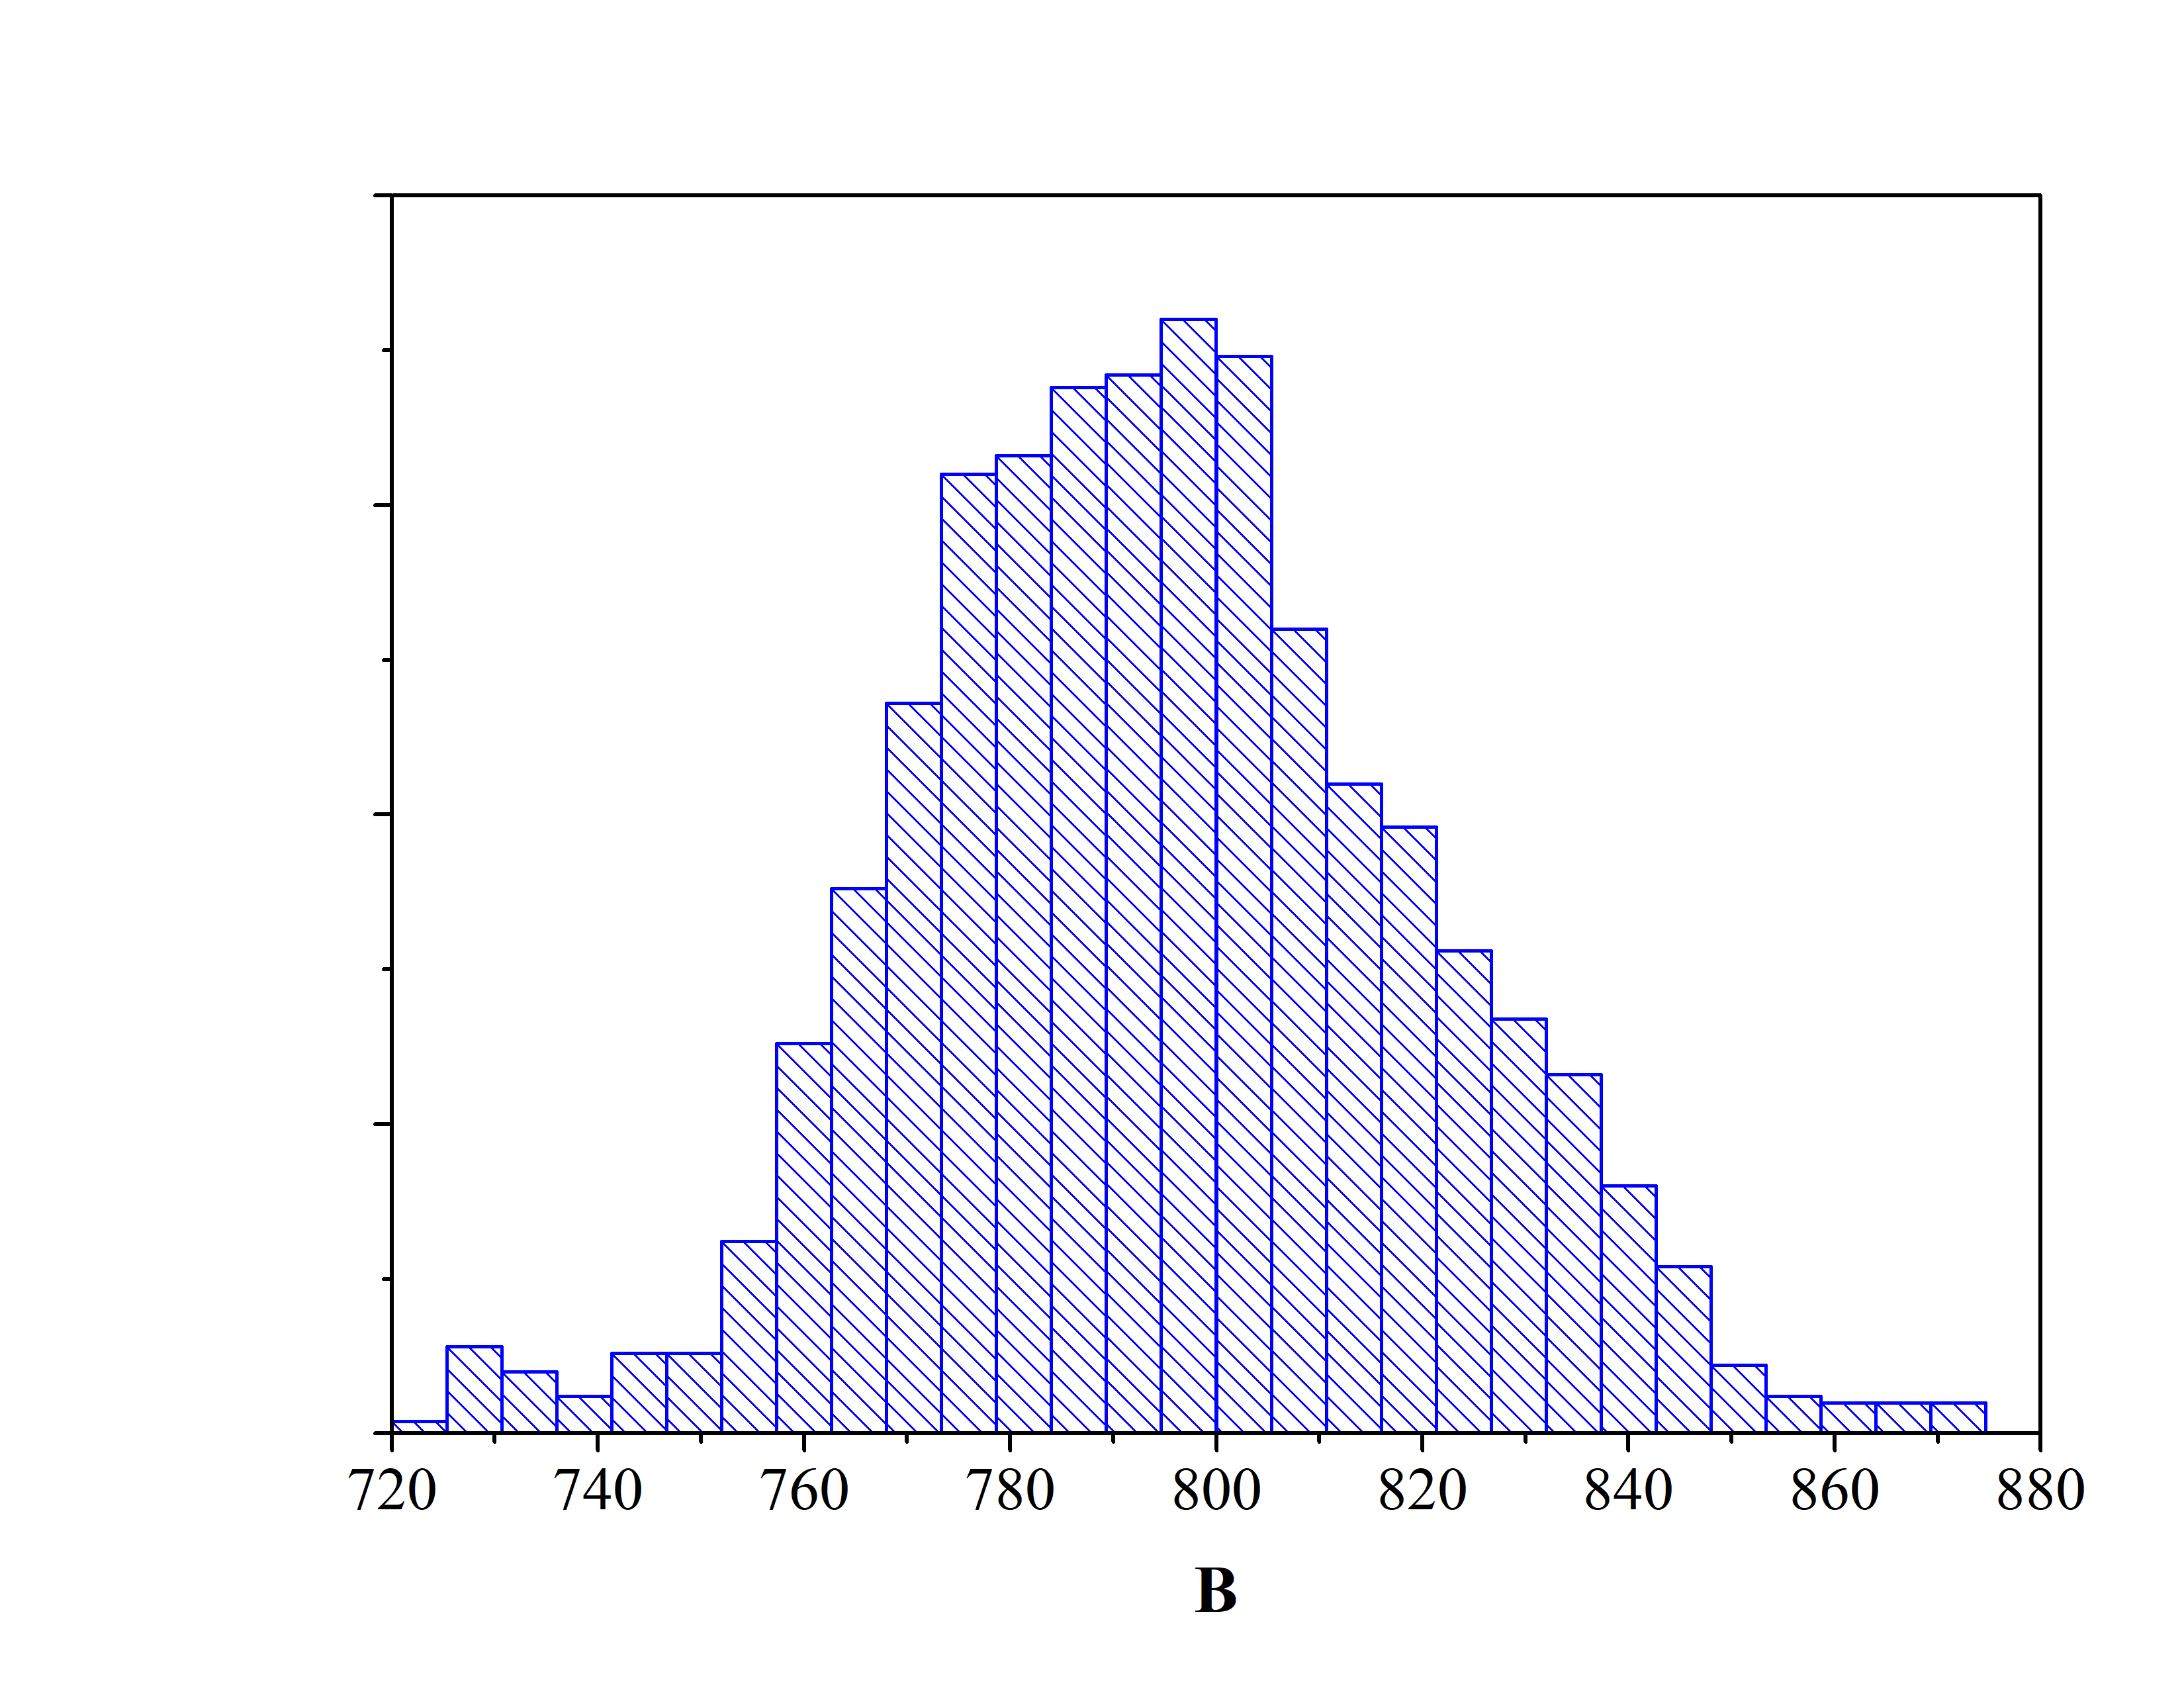
\includegraphics[width=0.3\textwidth]{./figs/posterior_A_B.png}}
\subfloat[Posterior of $\mathbf{n}$]{
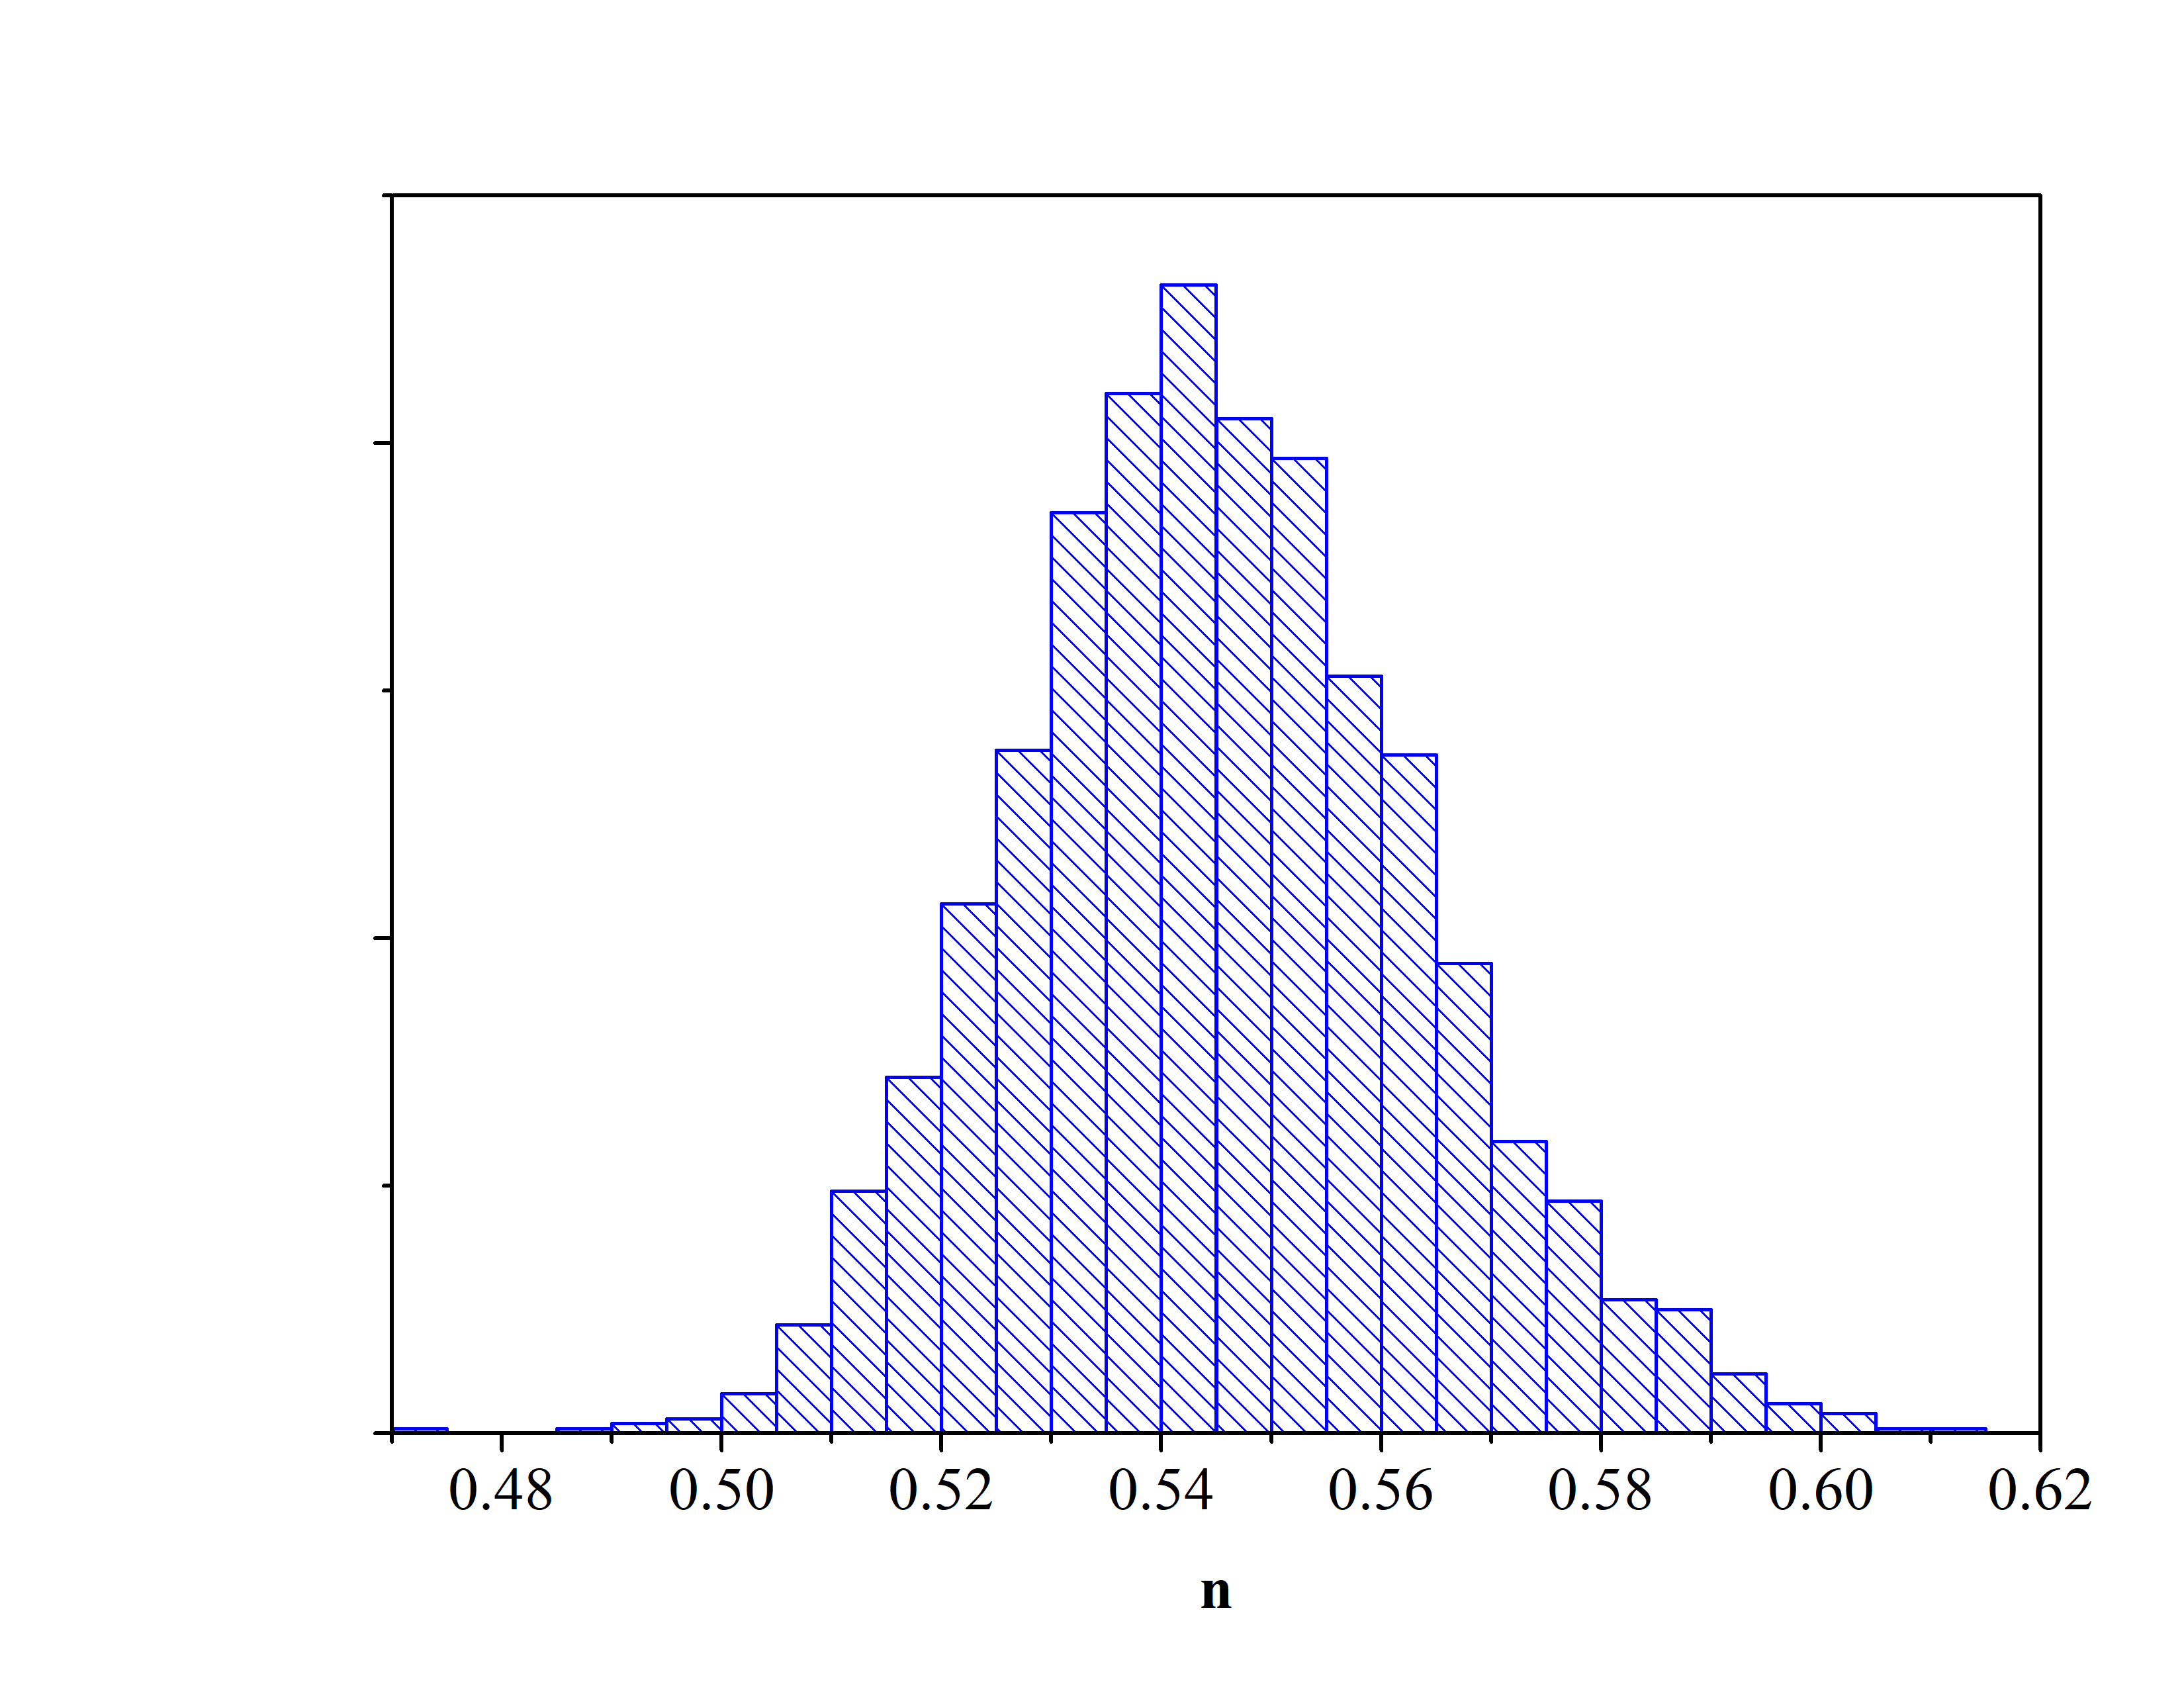
\includegraphics[width=0.3\textwidth]{./figs/posterior_A_n.png}}

Region A

\subfloat[Posterior of $\mathbf{A}$]{
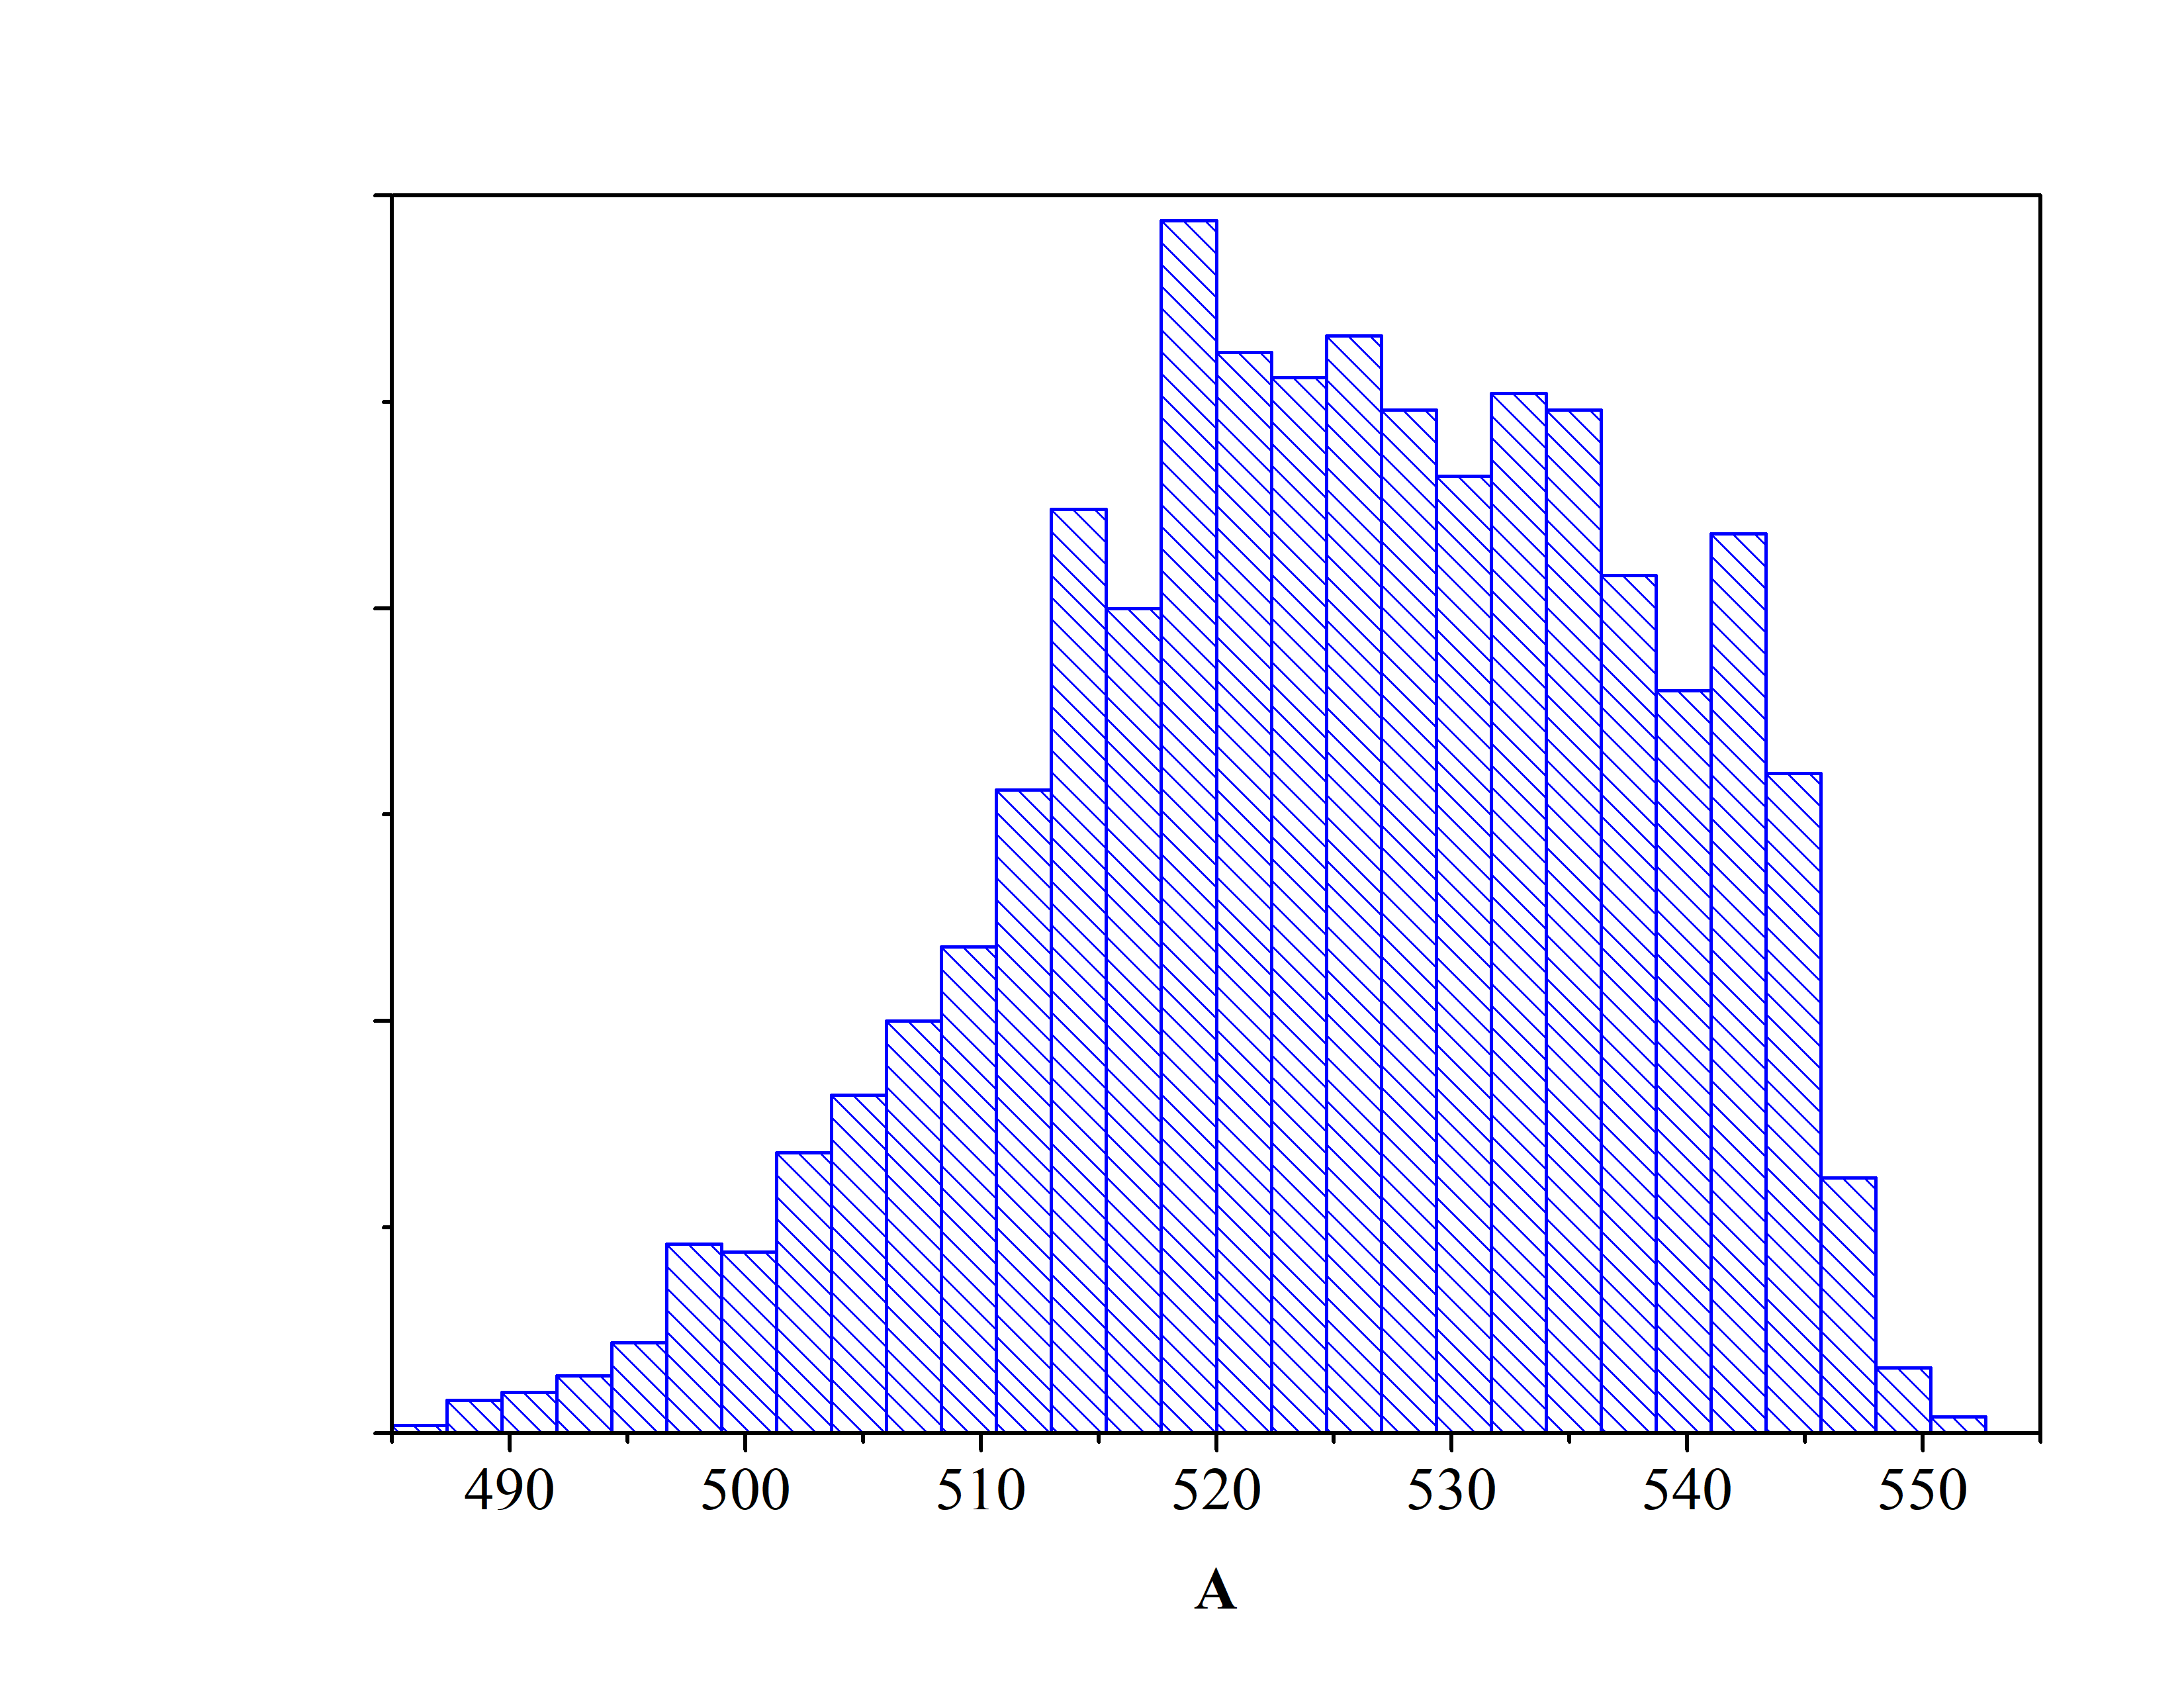
\includegraphics[width=0.3\textwidth]{./figs/posterior_B_A.png}}
\subfloat[Posterior of $\mathbf{B}$]{
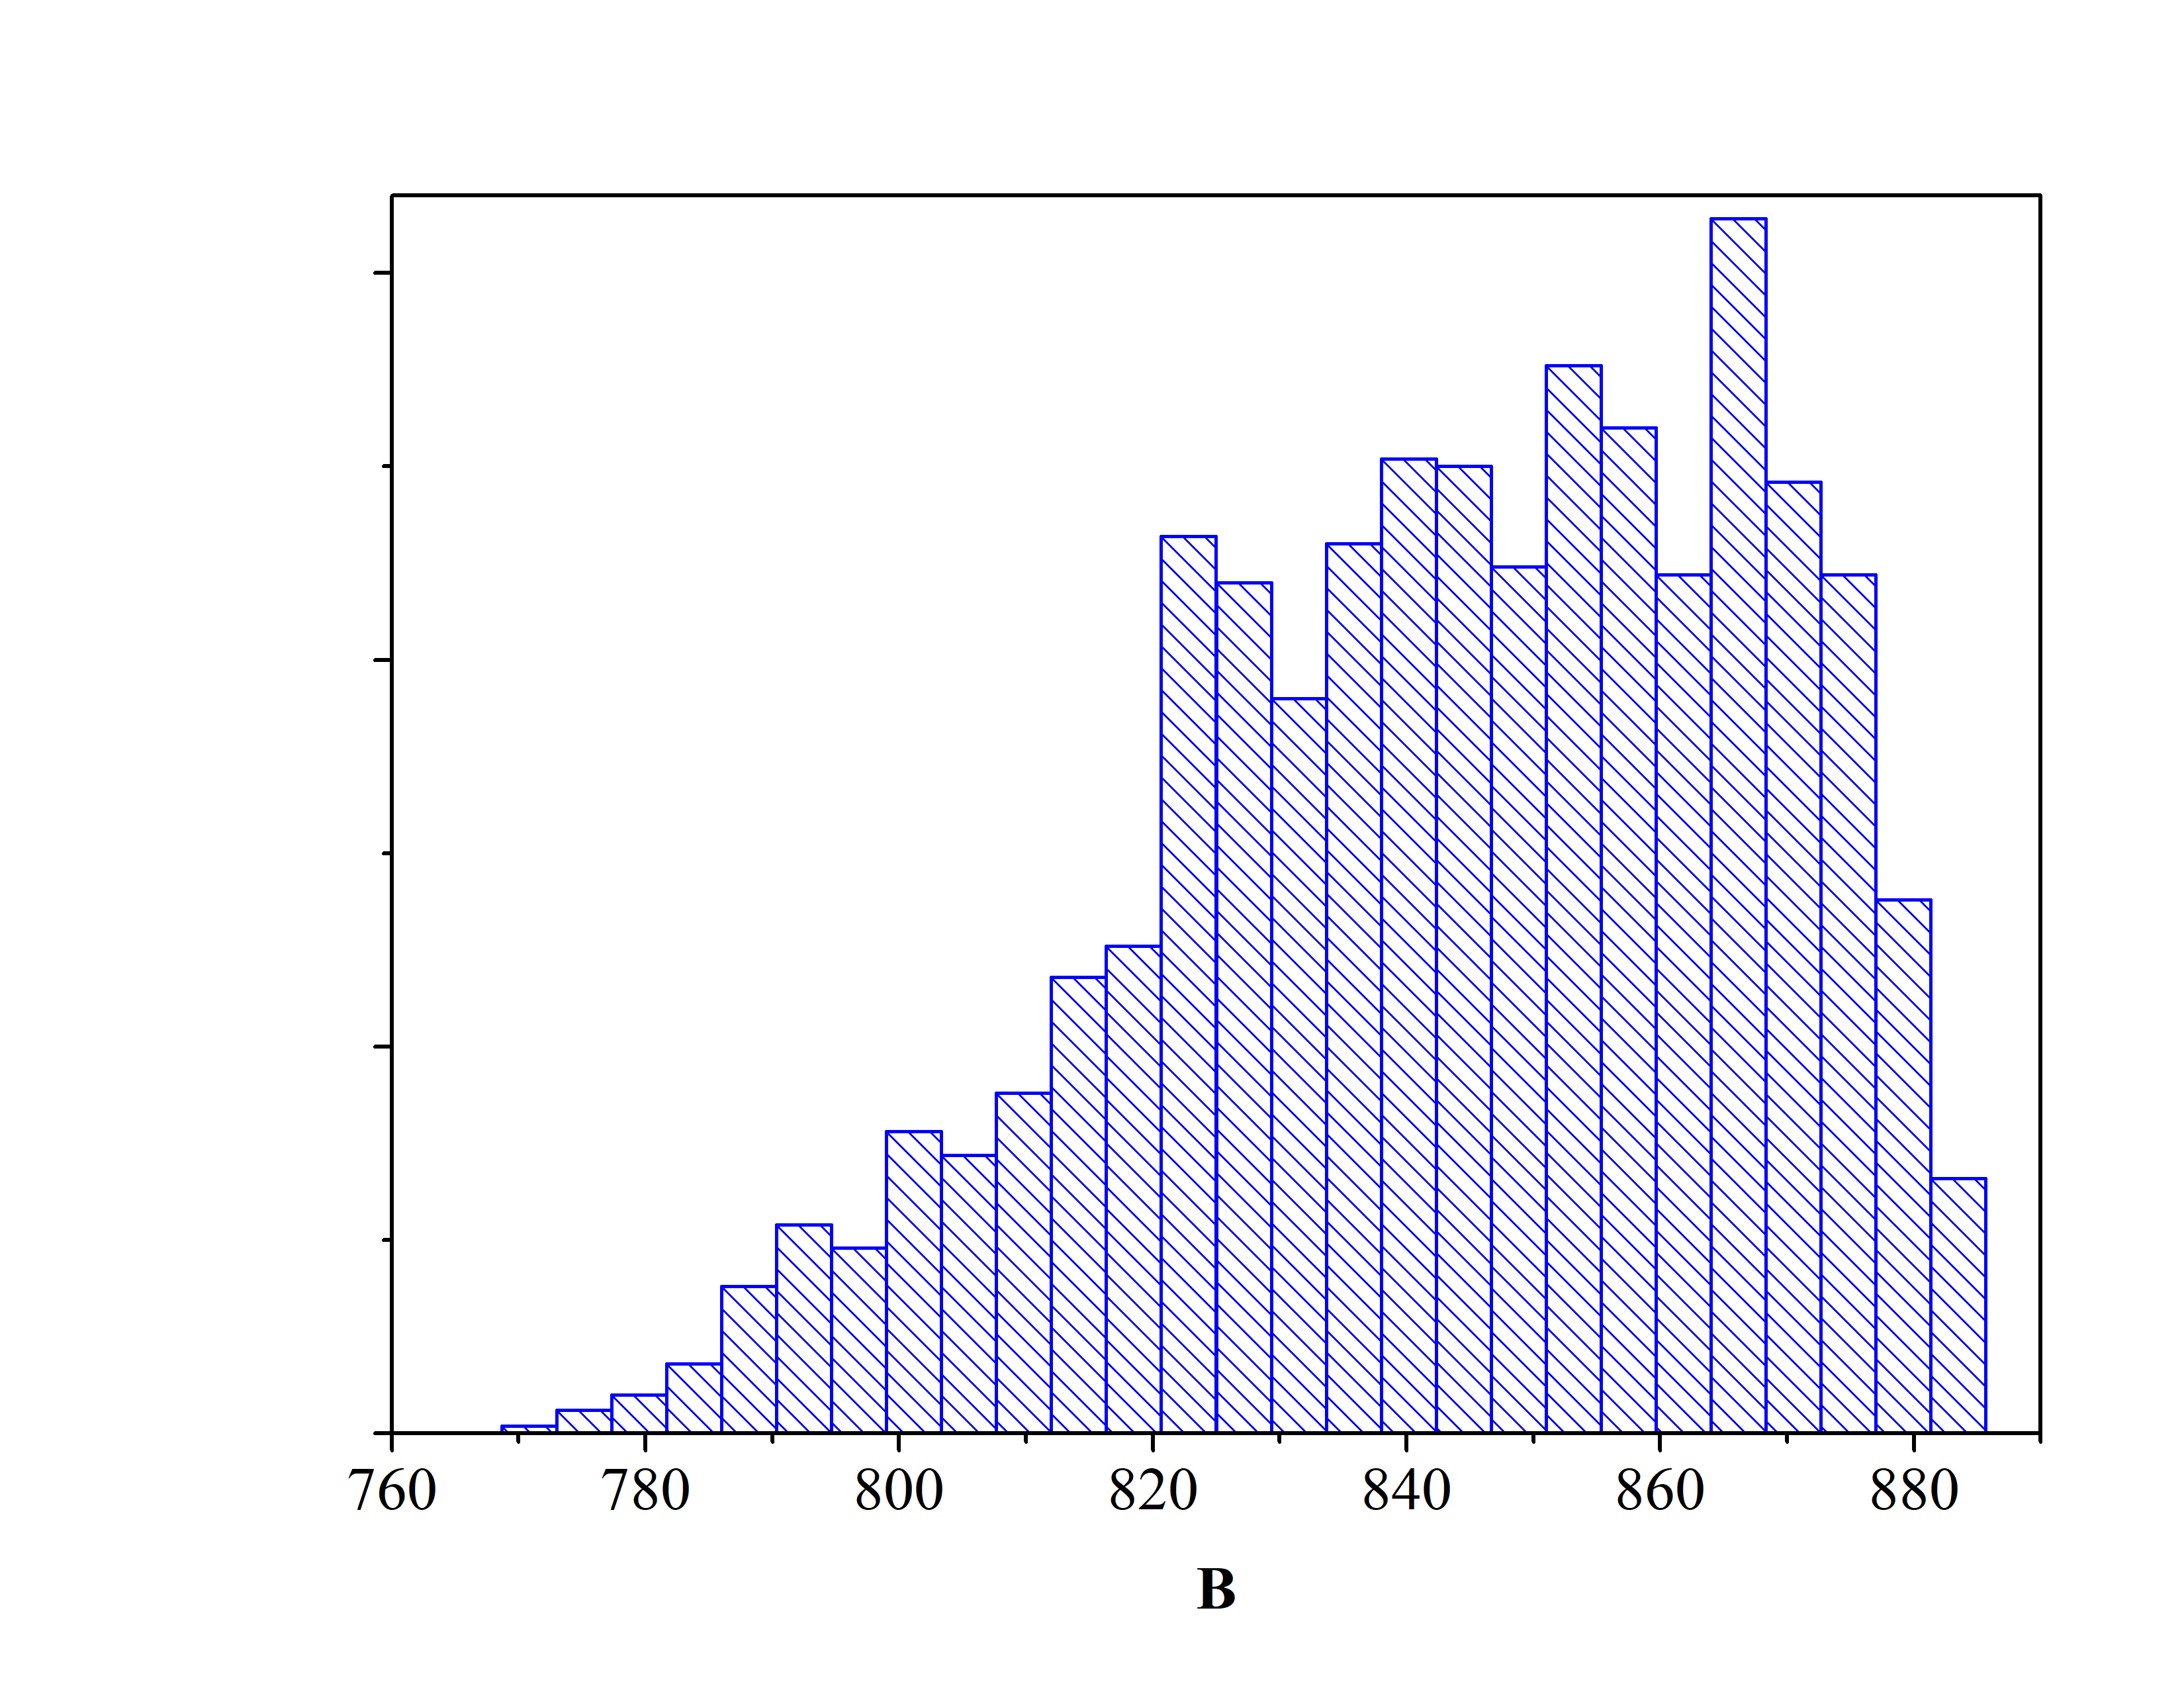
\includegraphics[width=0.3\textwidth]{./figs/posterior_B_B.png}}
\subfloat[Posterior of $\mathbf{n}$]{
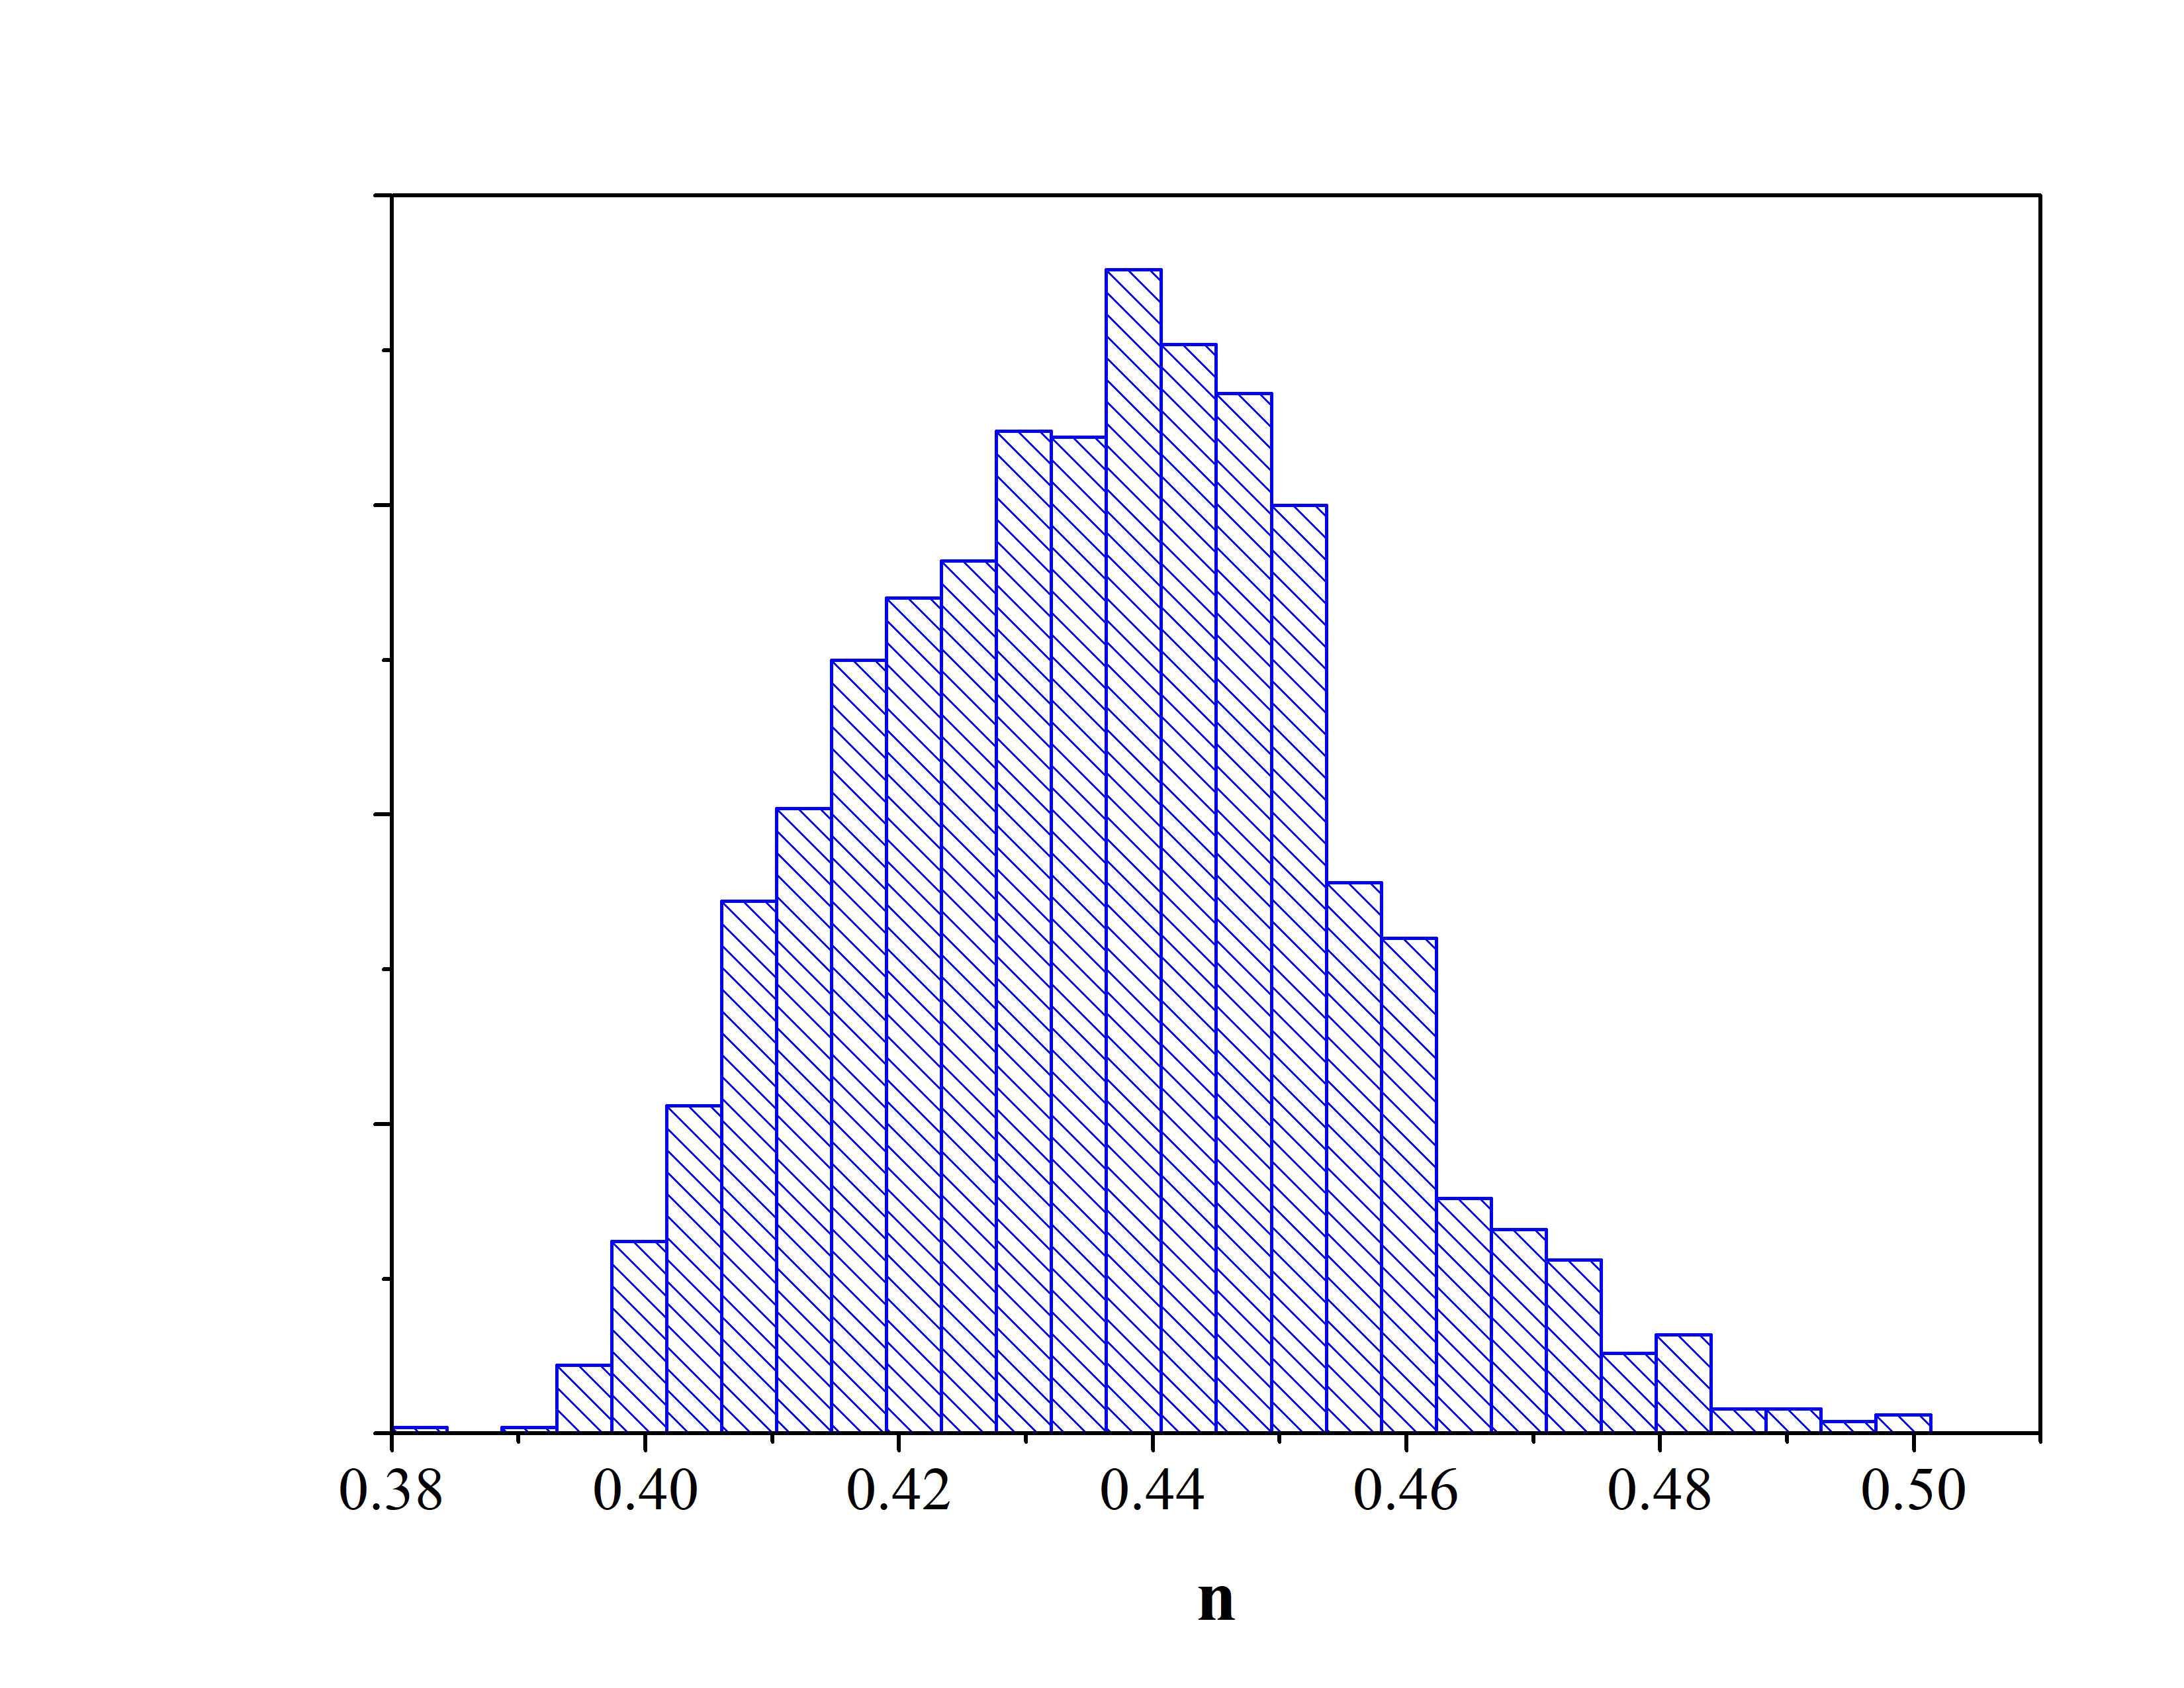
\includegraphics[width=0.3\textwidth]{./figs/posterior_B_n.png}}

Region B

\subfloat[Posterior of $\mathbf{A}$]{
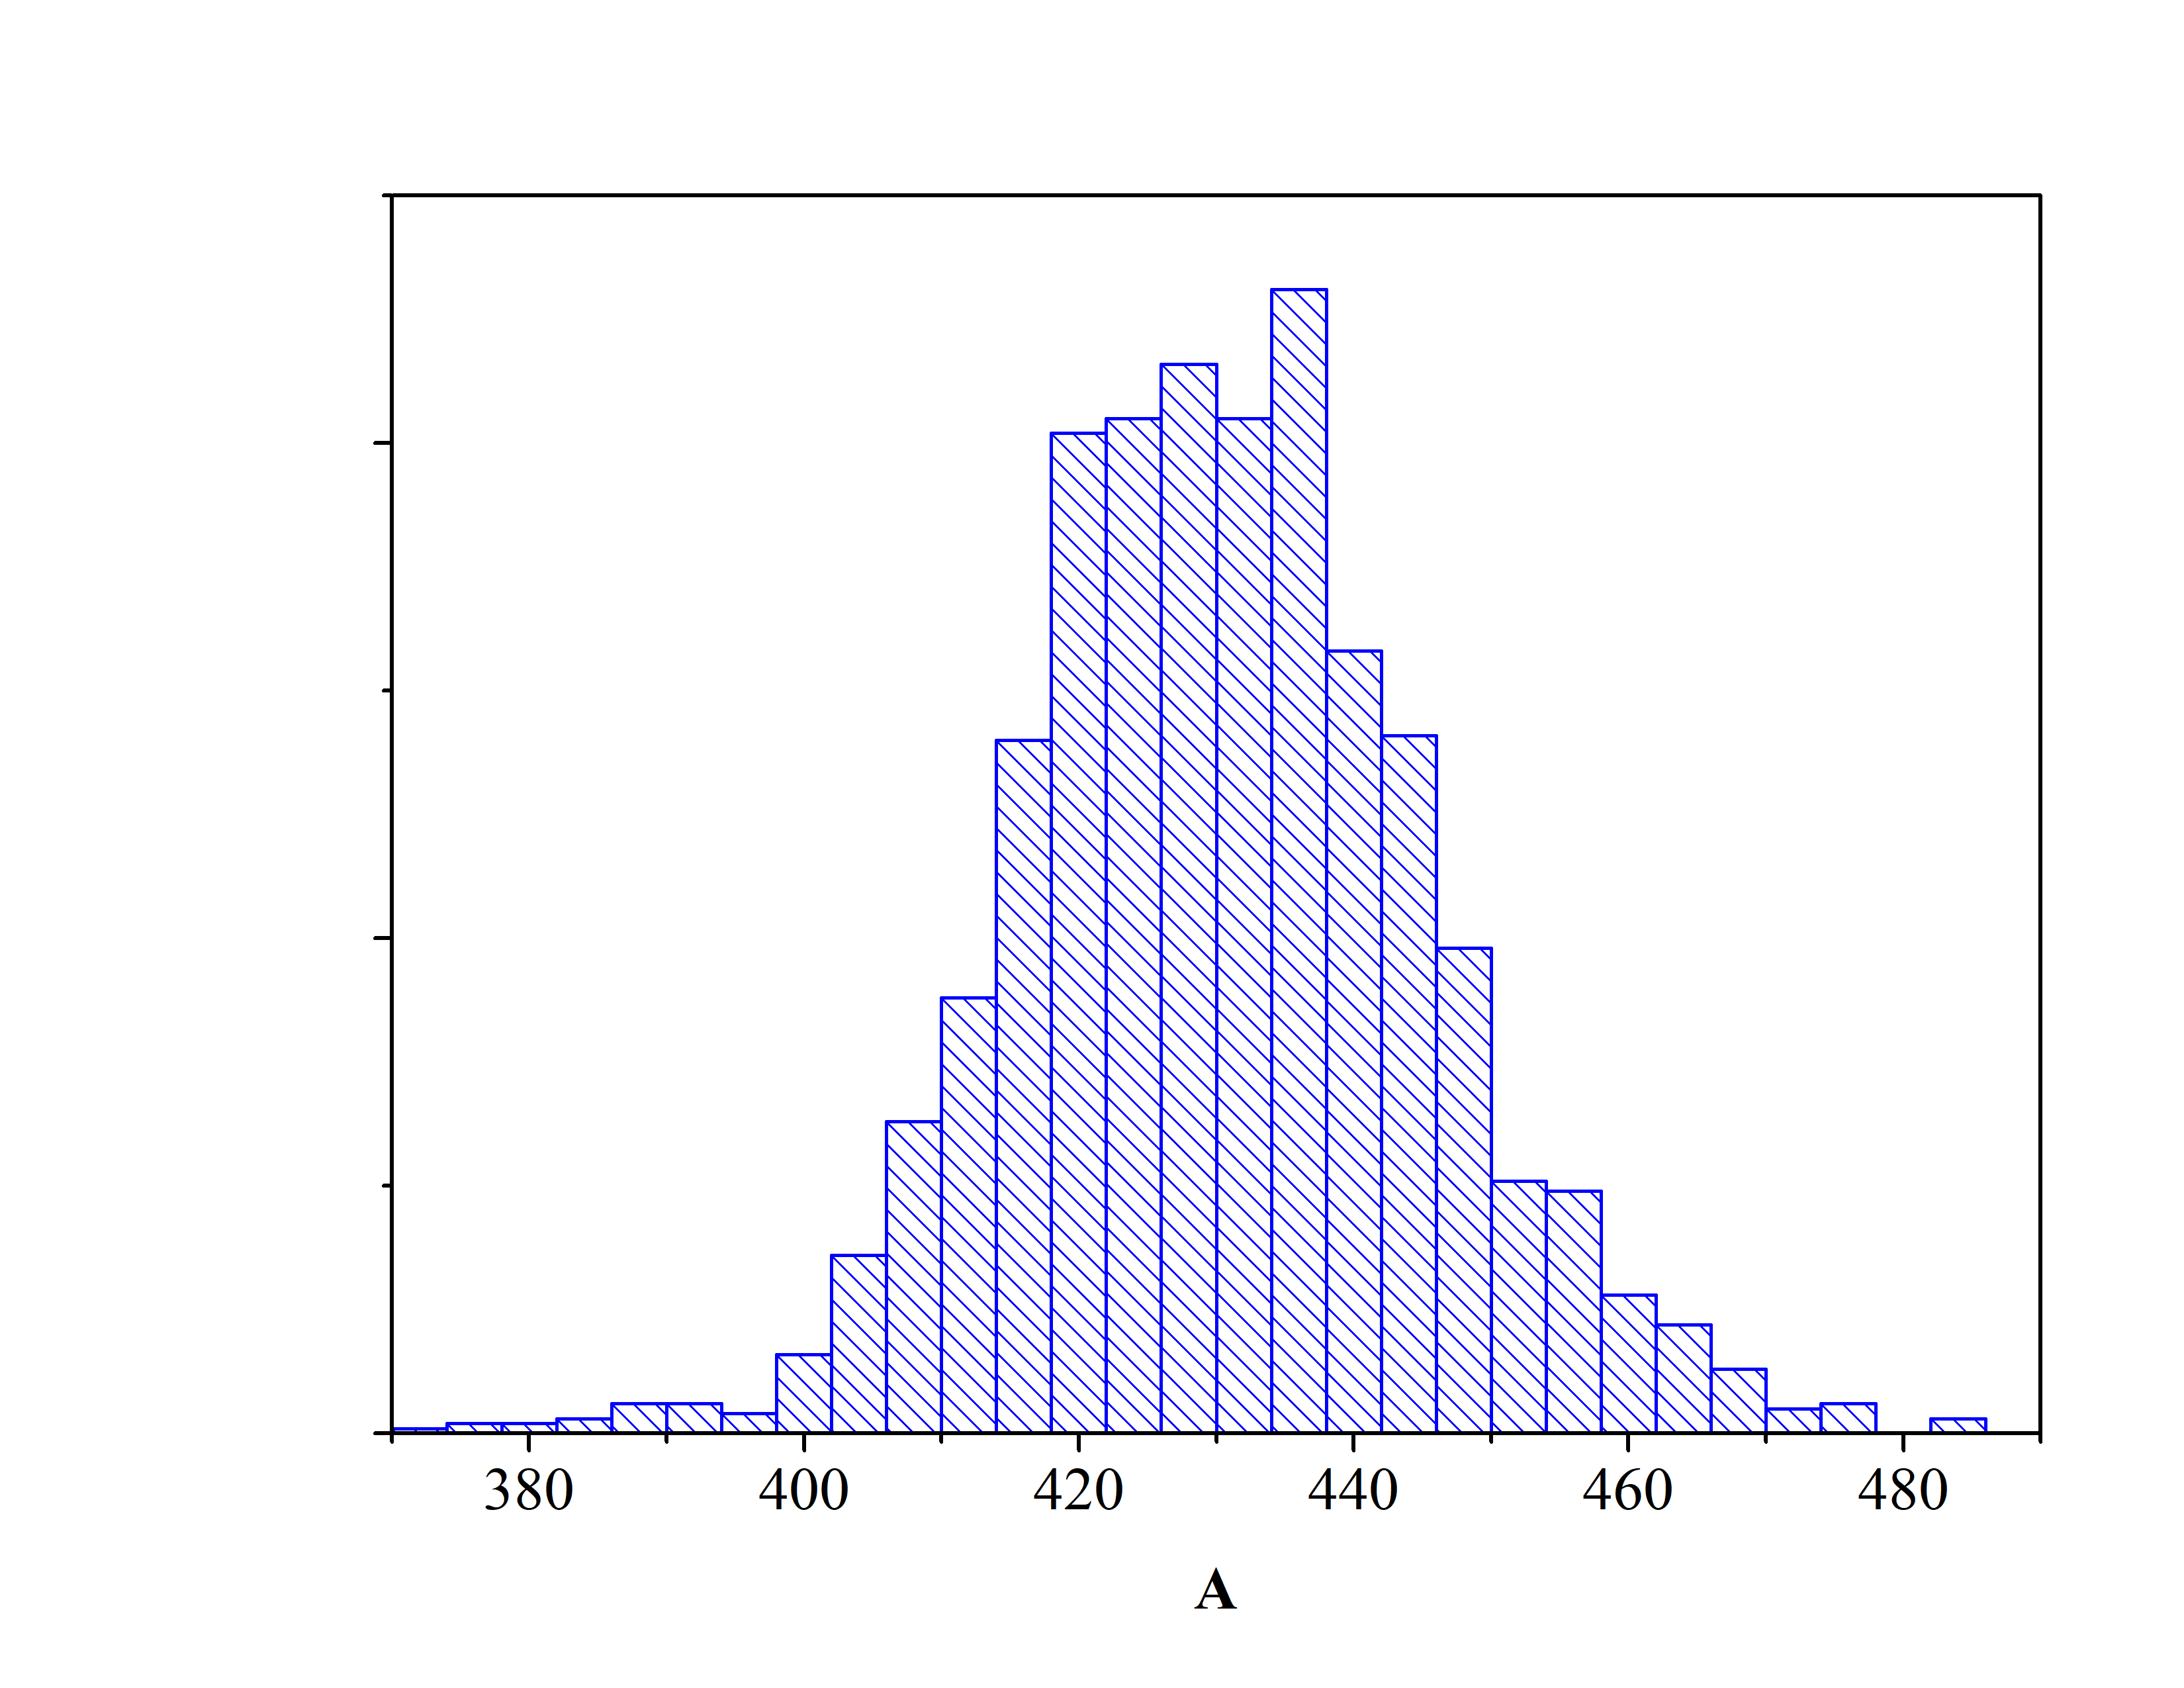
\includegraphics[width=0.3\textwidth]{./figs/posterior_C_A.png}}
\subfloat[Posterior of $\mathbf{B}$]{
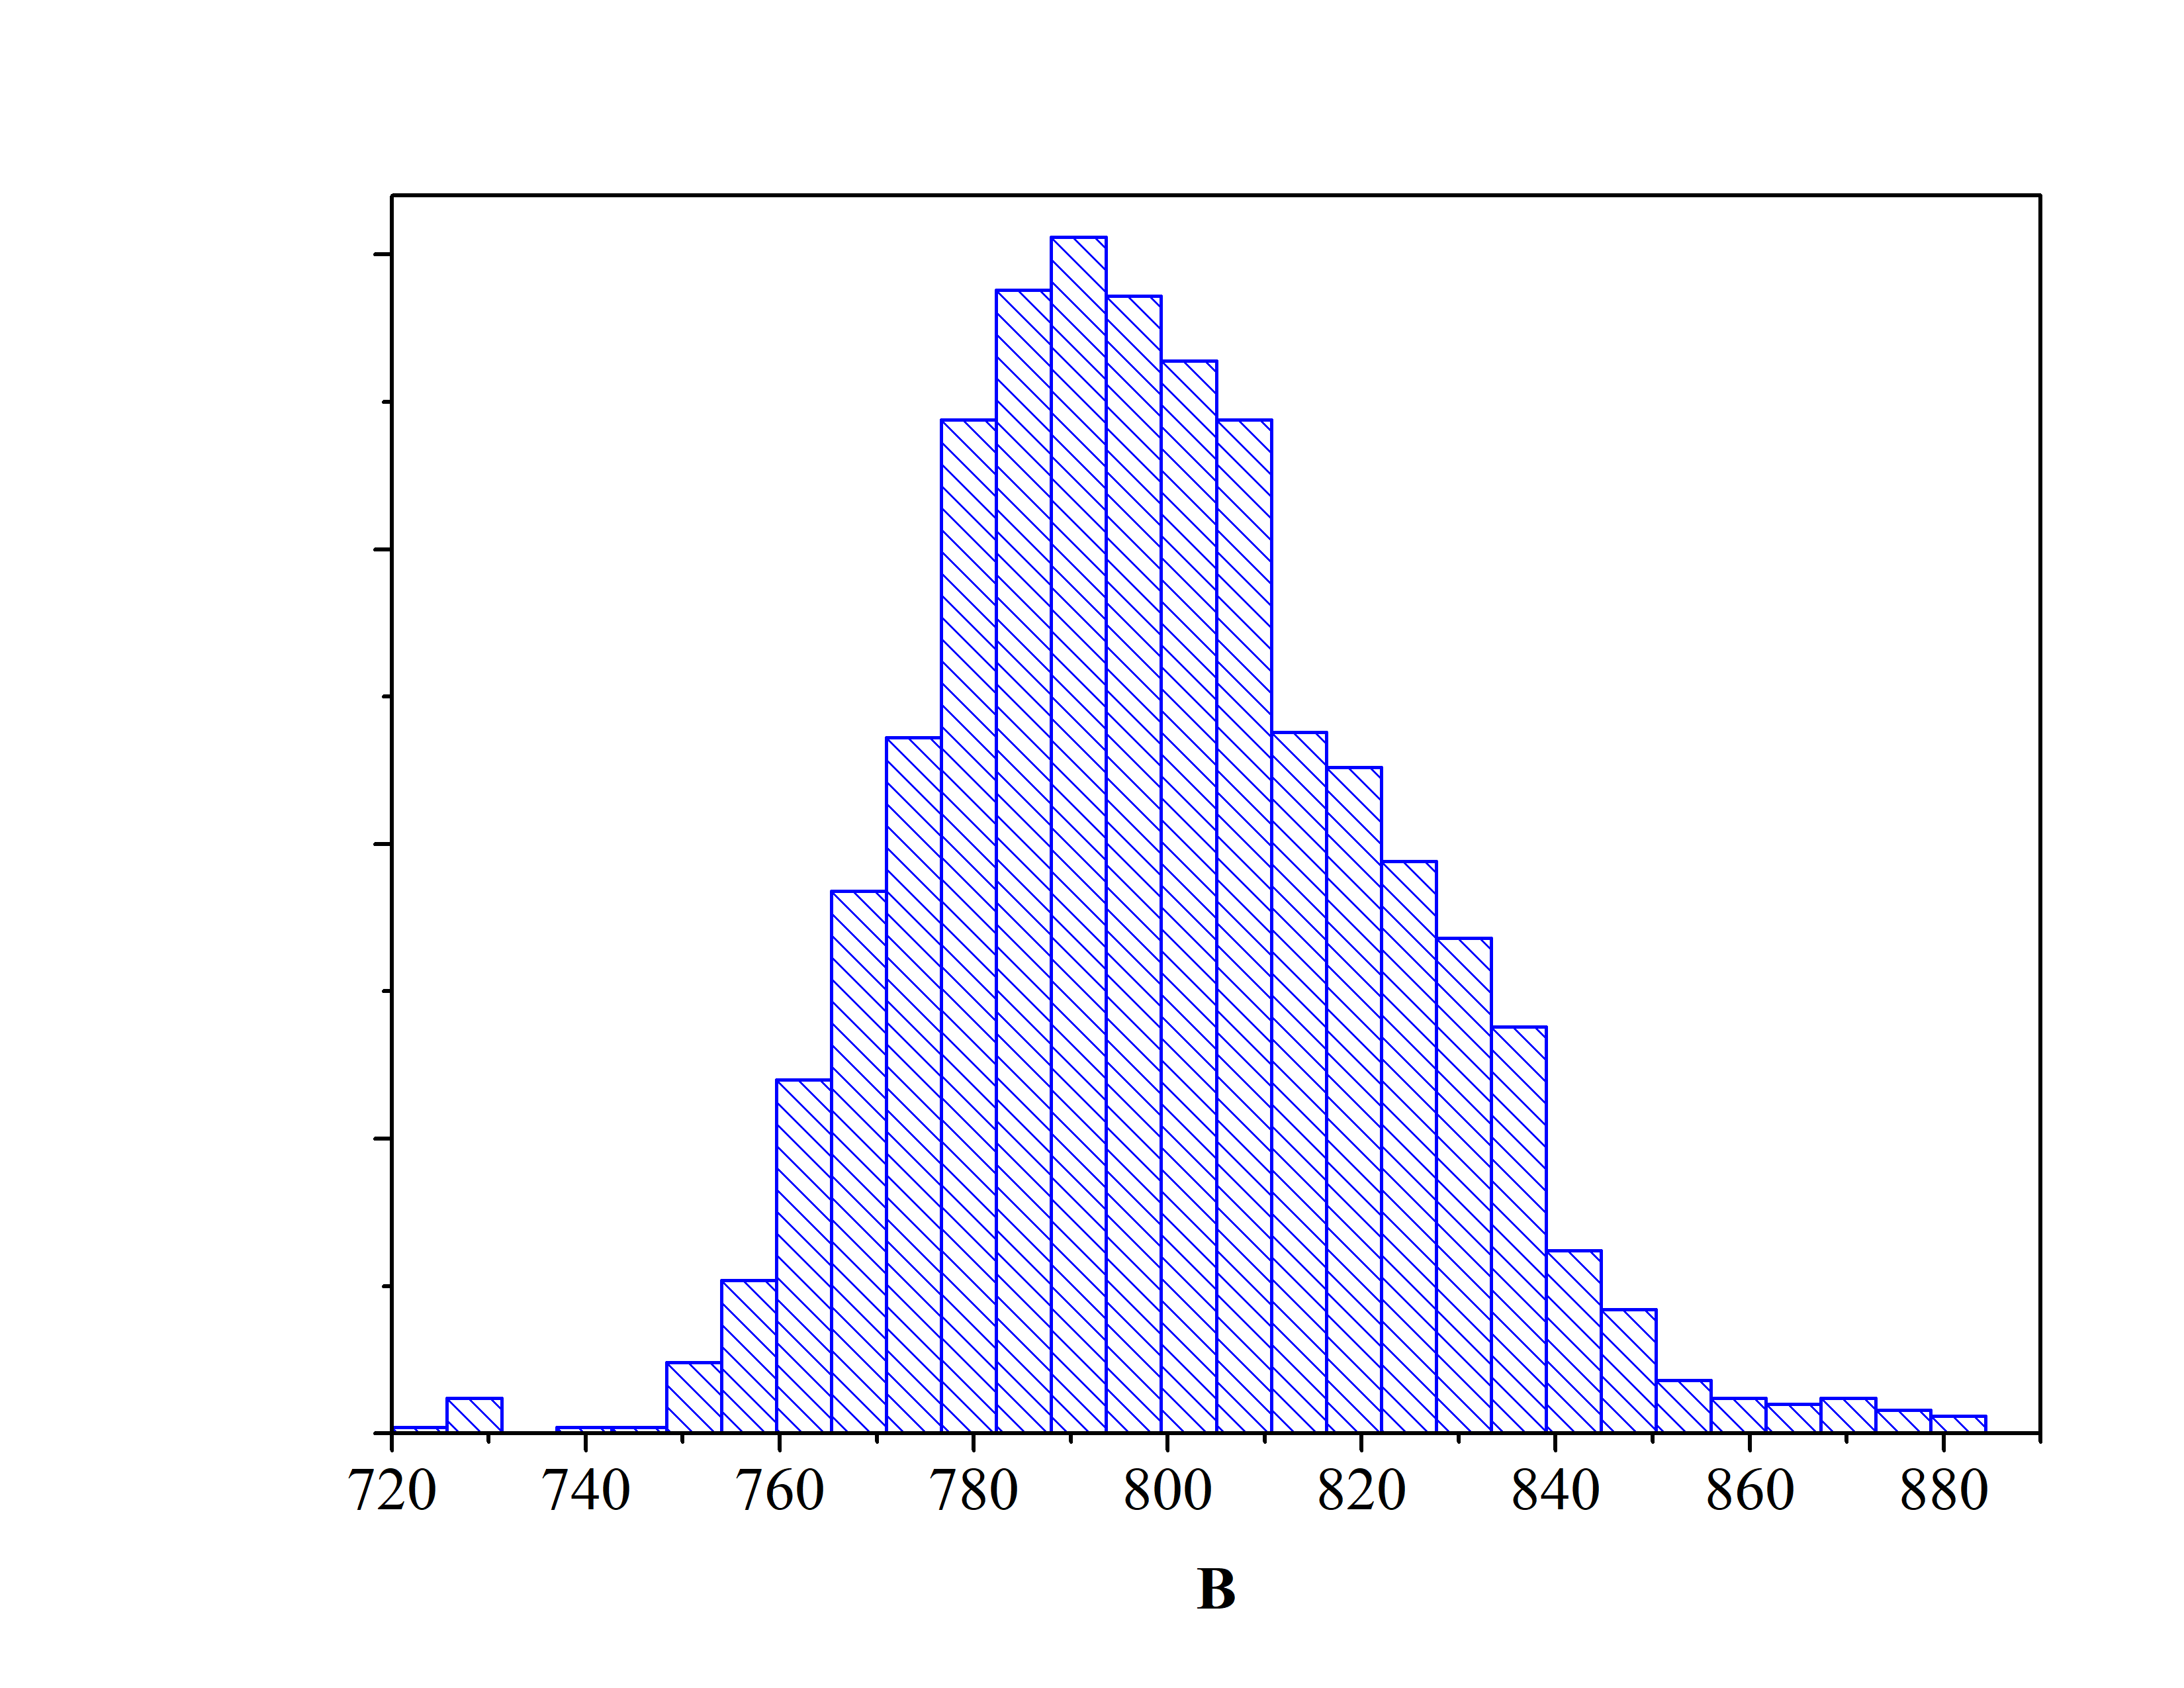
\includegraphics[width=0.3\textwidth]{./figs/posterior_C_B.png}}
\subfloat[Posterior of $\mathbf{n}$]{
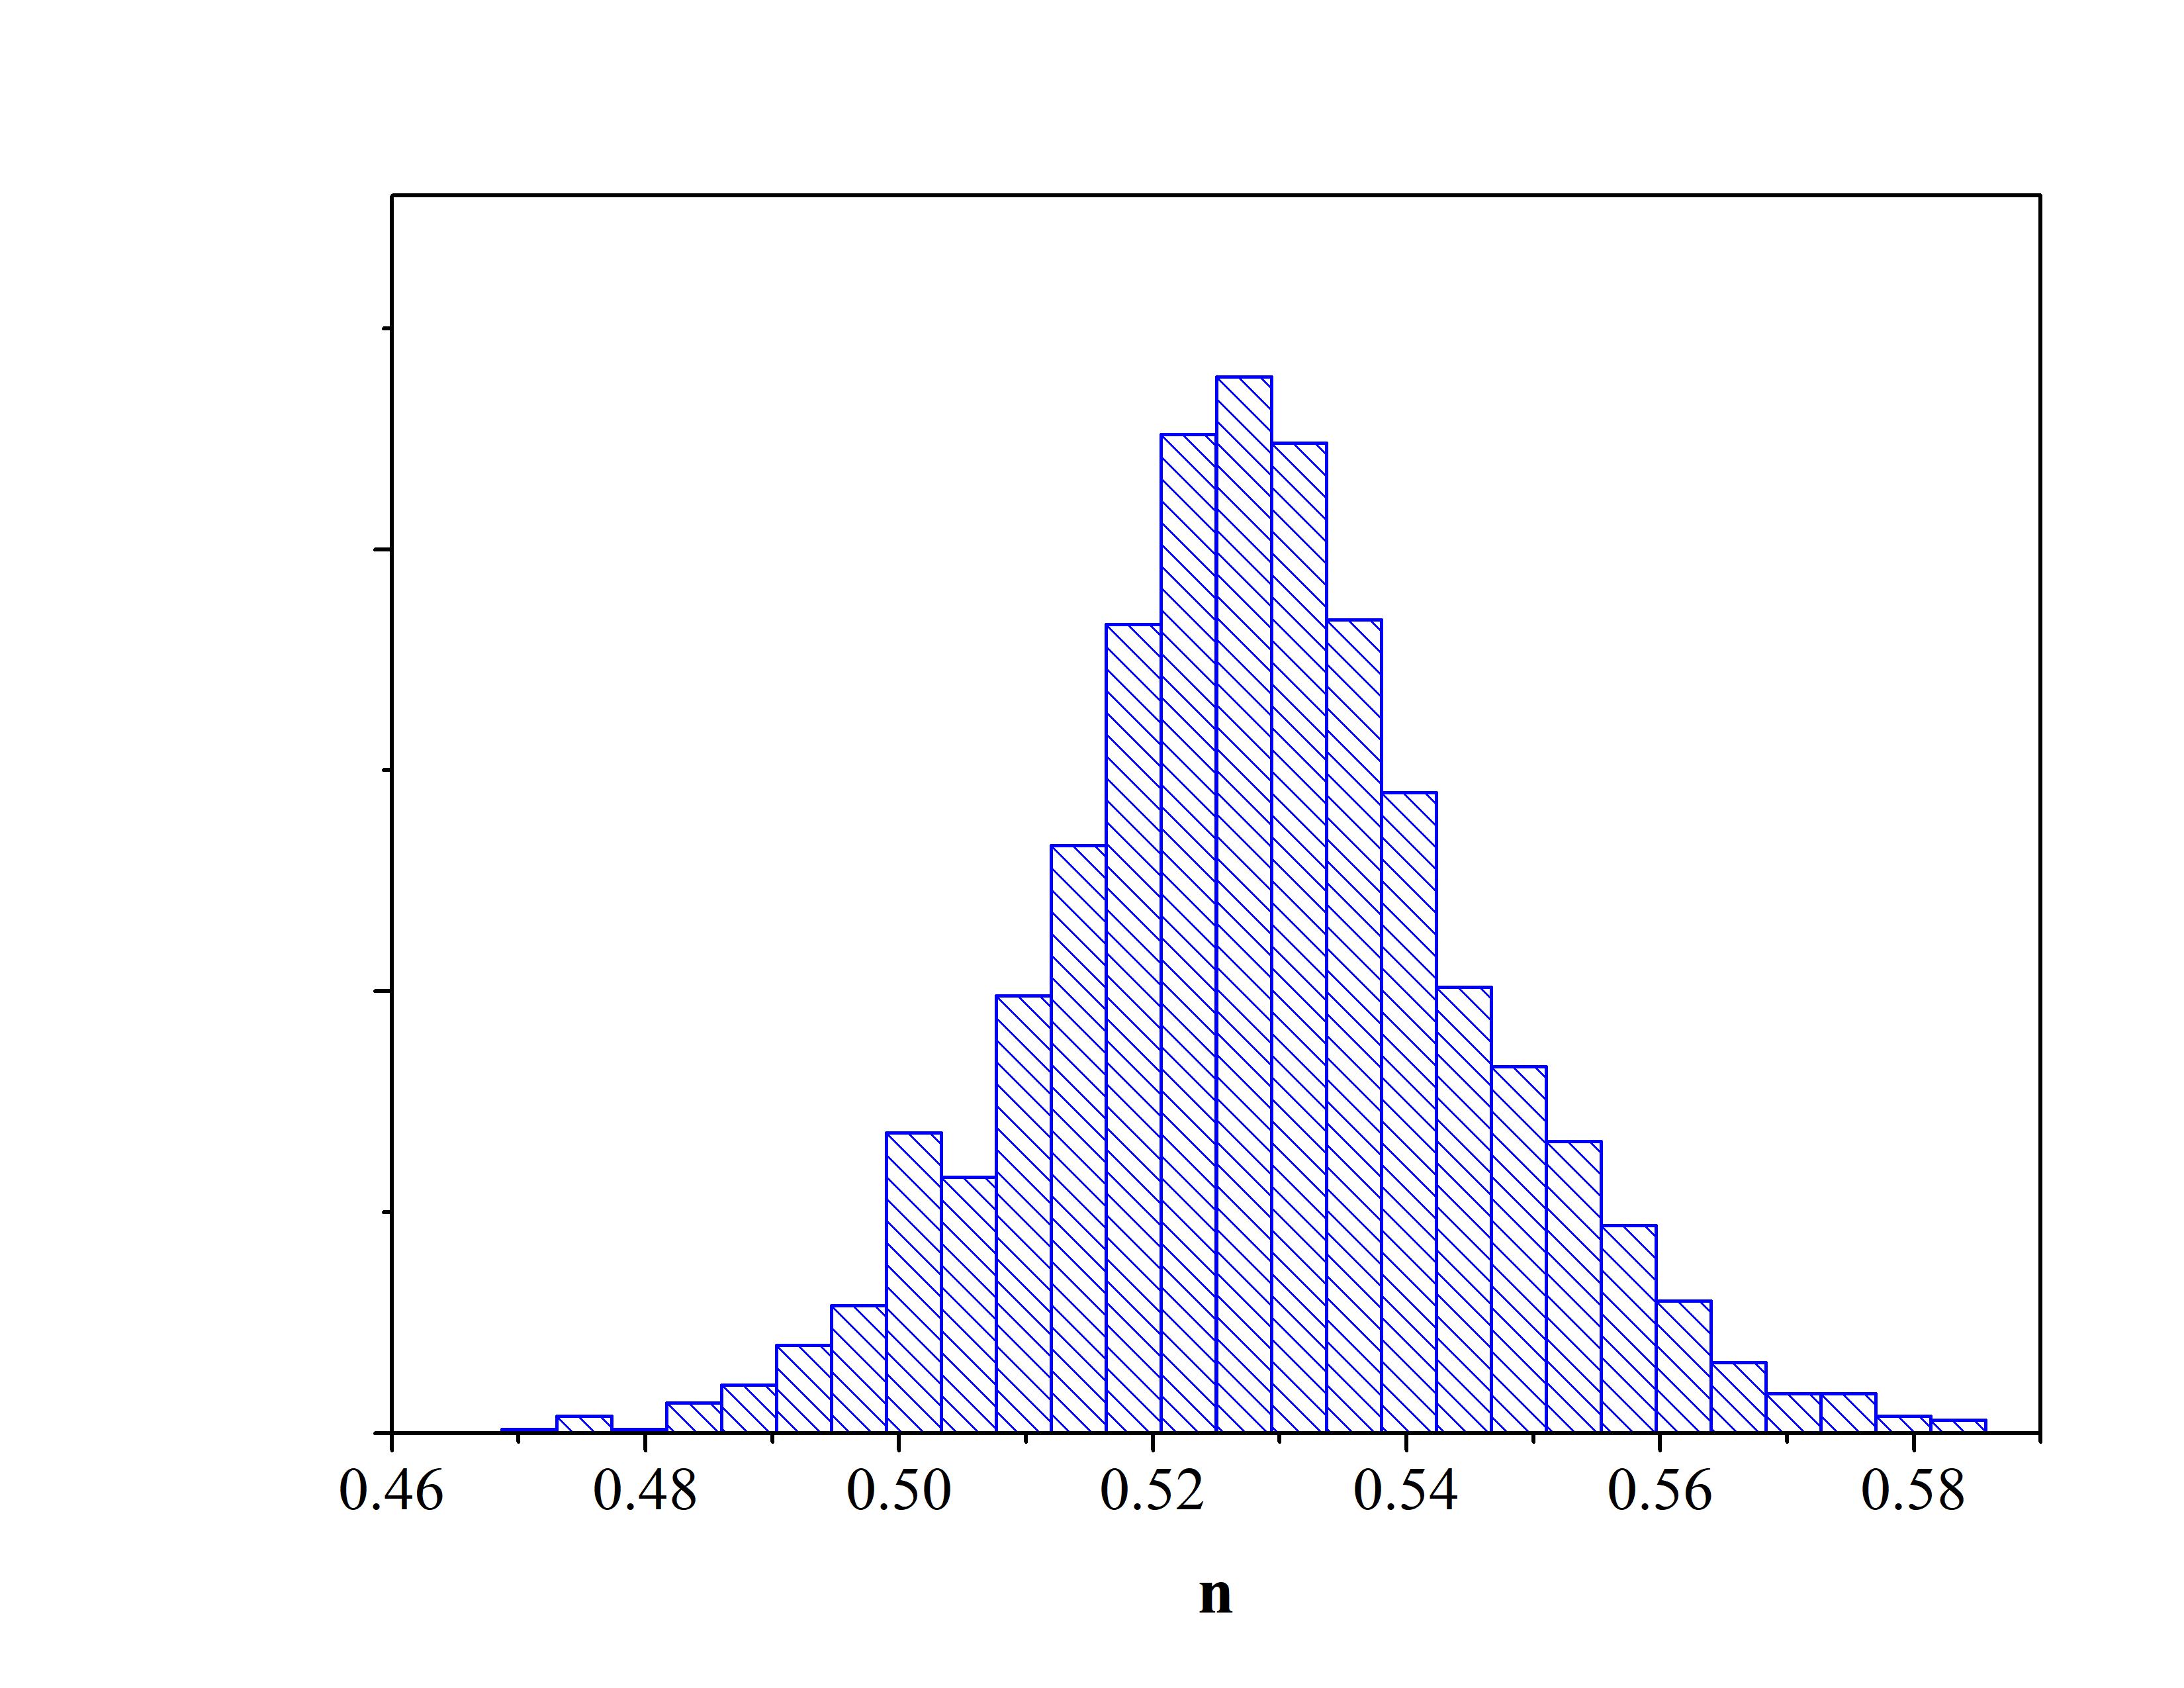
\includegraphics[width=0.3\textwidth]{./figs/posterior_C_n.png}}

Region C

\caption{Posteriors of the formed specimen}
\label{fig:posterior formed}
\end{figure}

\begin{figure}[h!]
\centering
\subfloat[Raw specimen]{
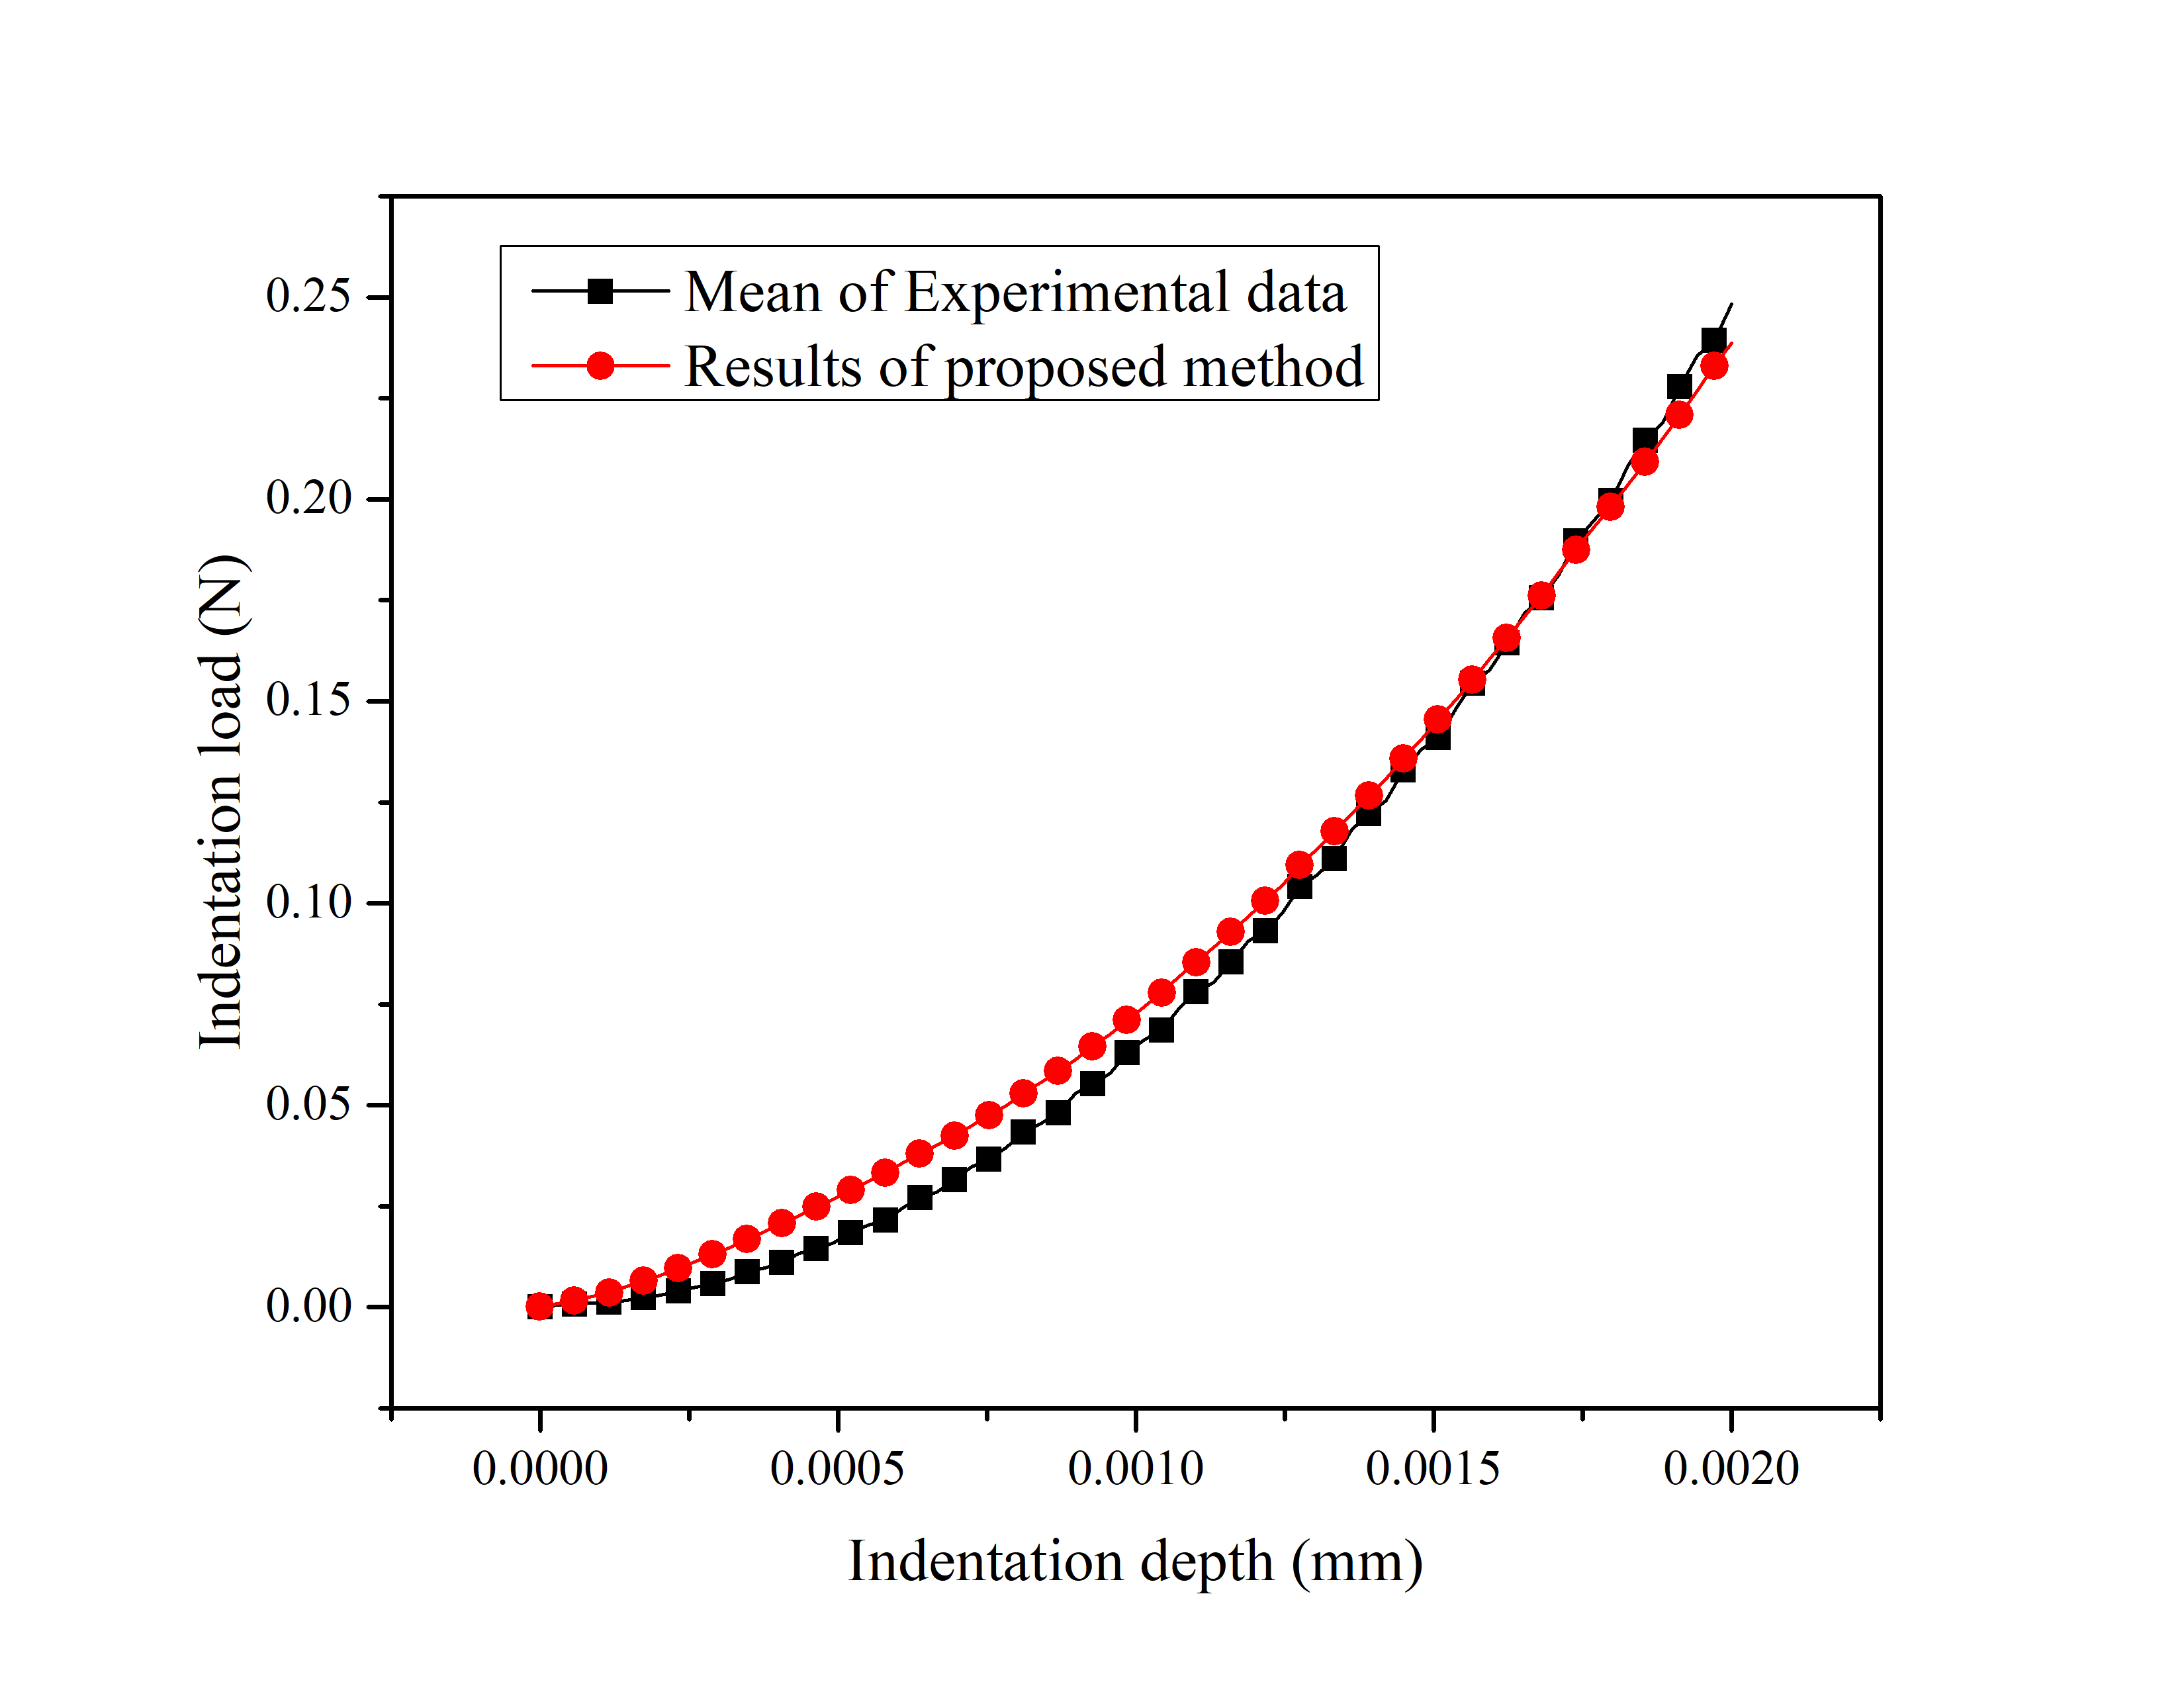
\includegraphics[width=0.45\textwidth]{./figs/results_DP.png}}
\subfloat[Region A]{
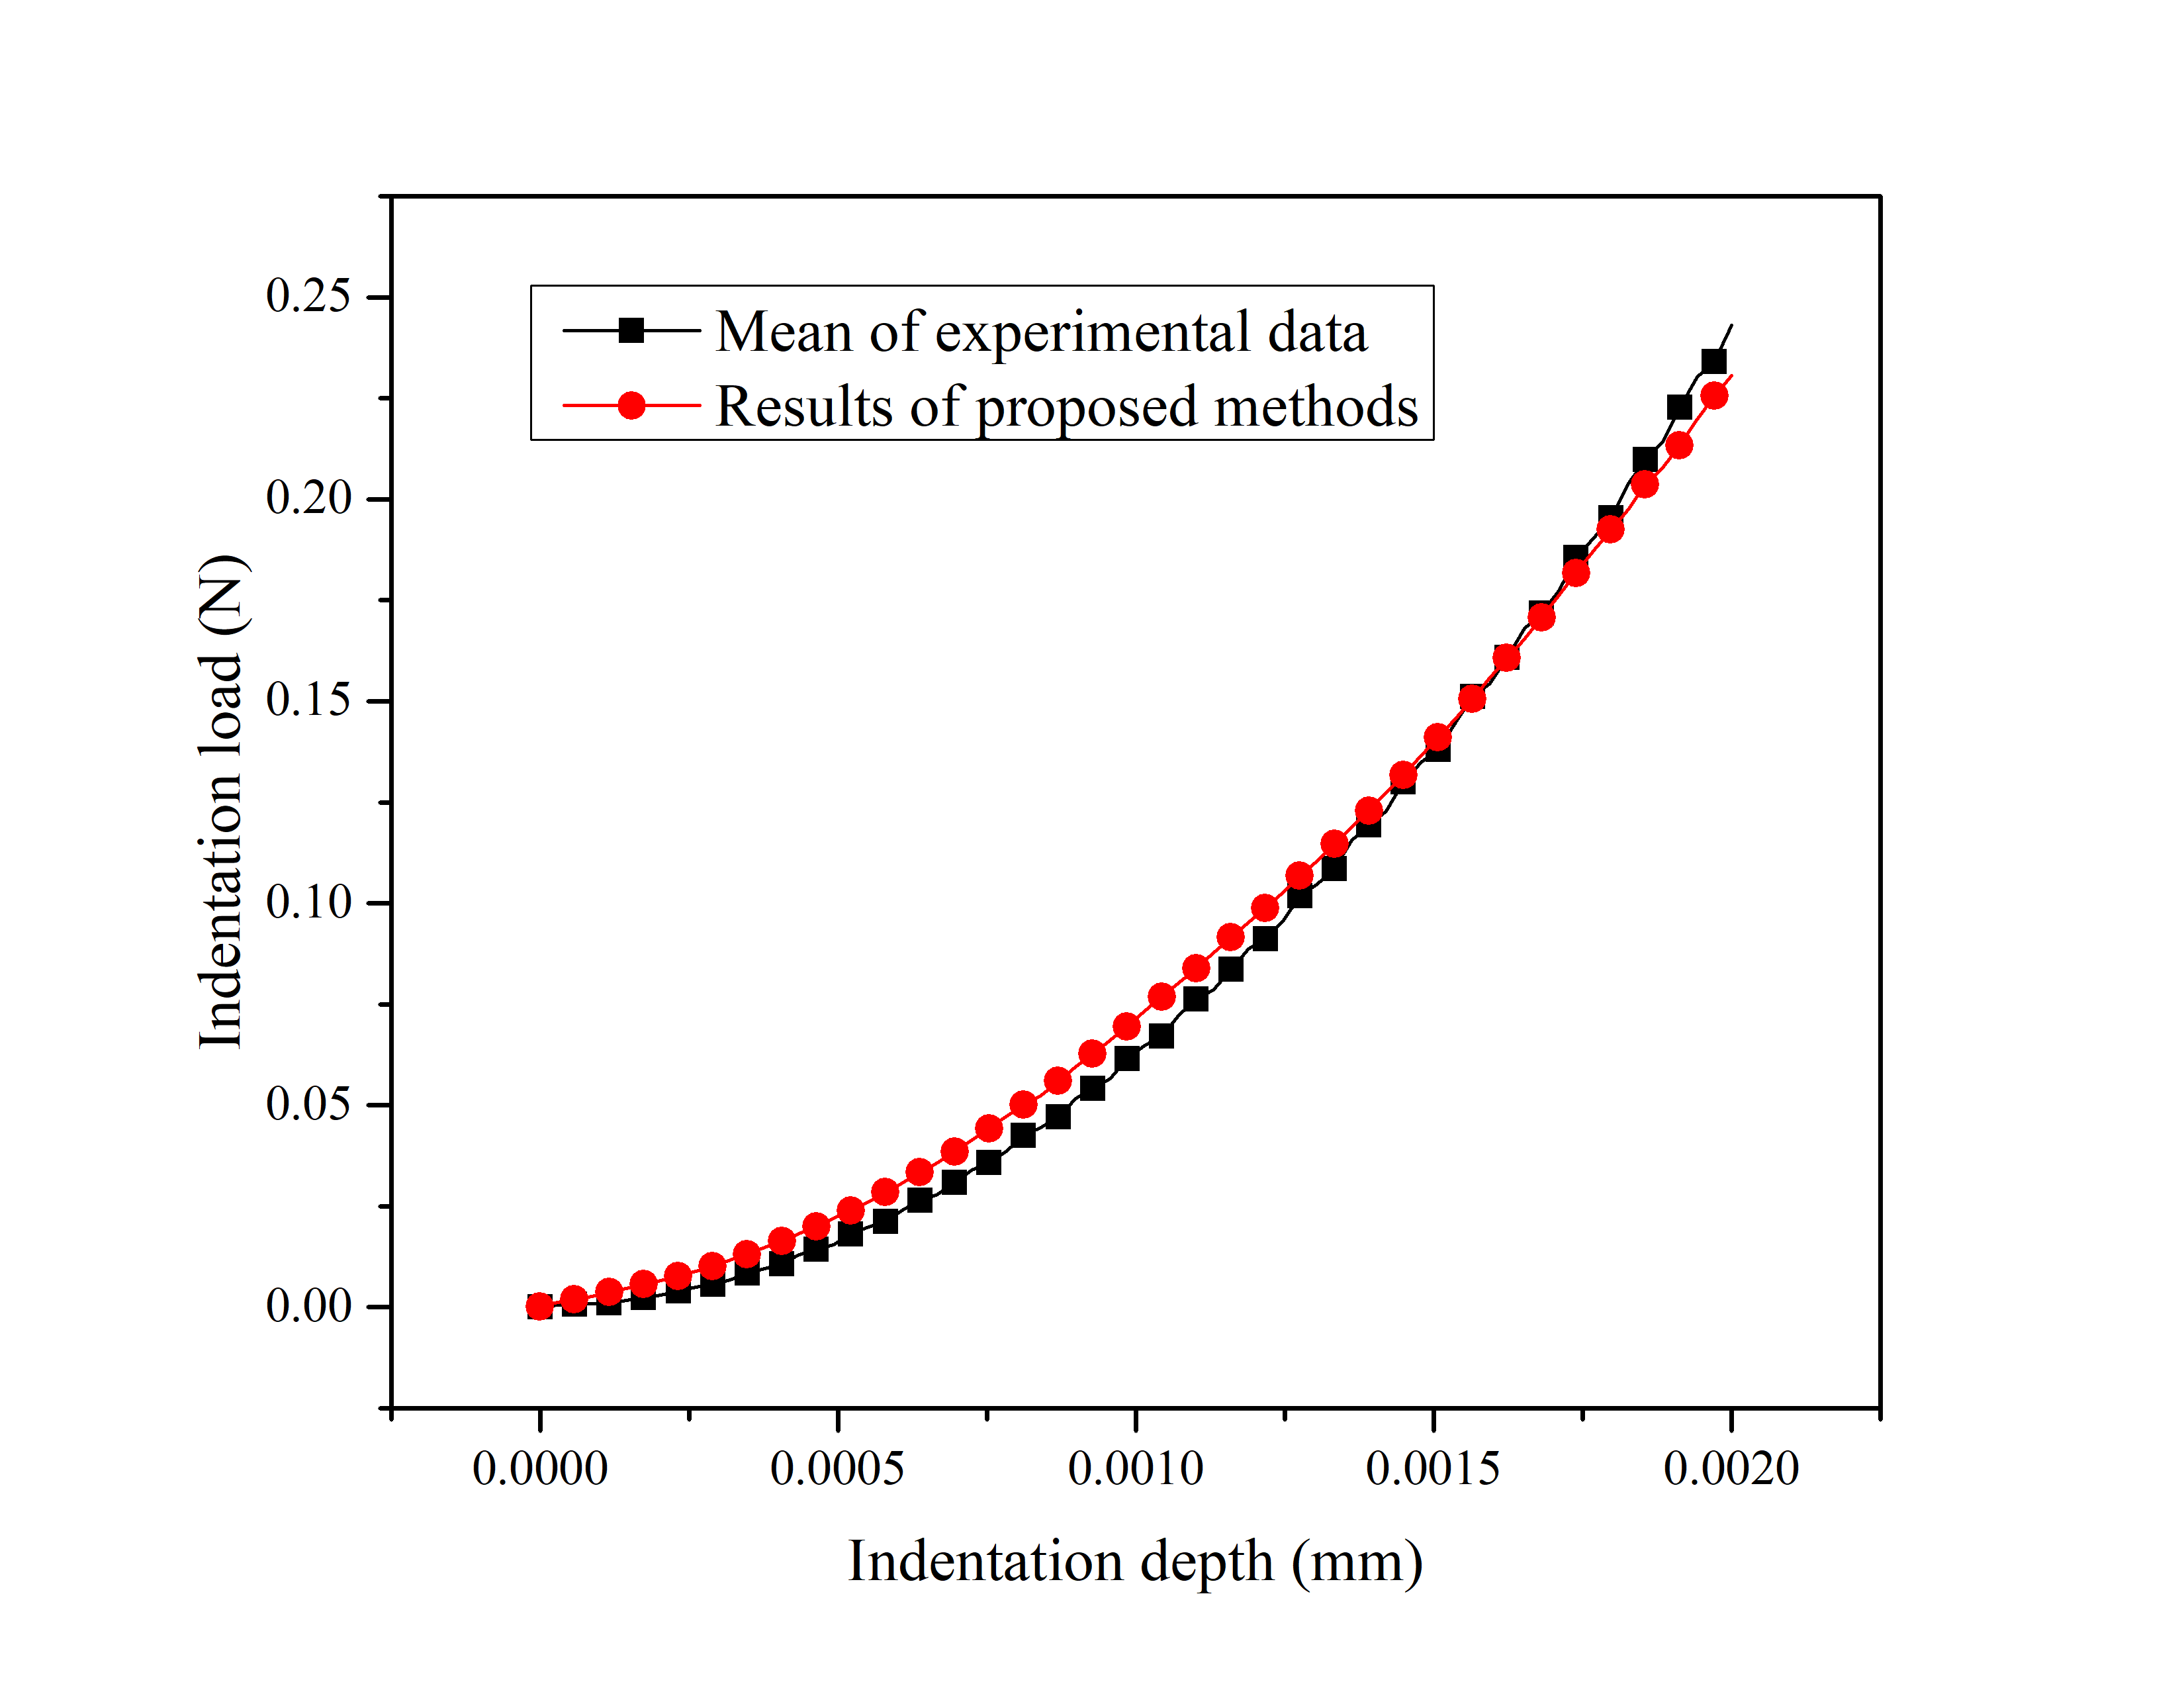
\includegraphics[width=0.45\textwidth]{./figs/result_A.png}}

\subfloat[Region B]{
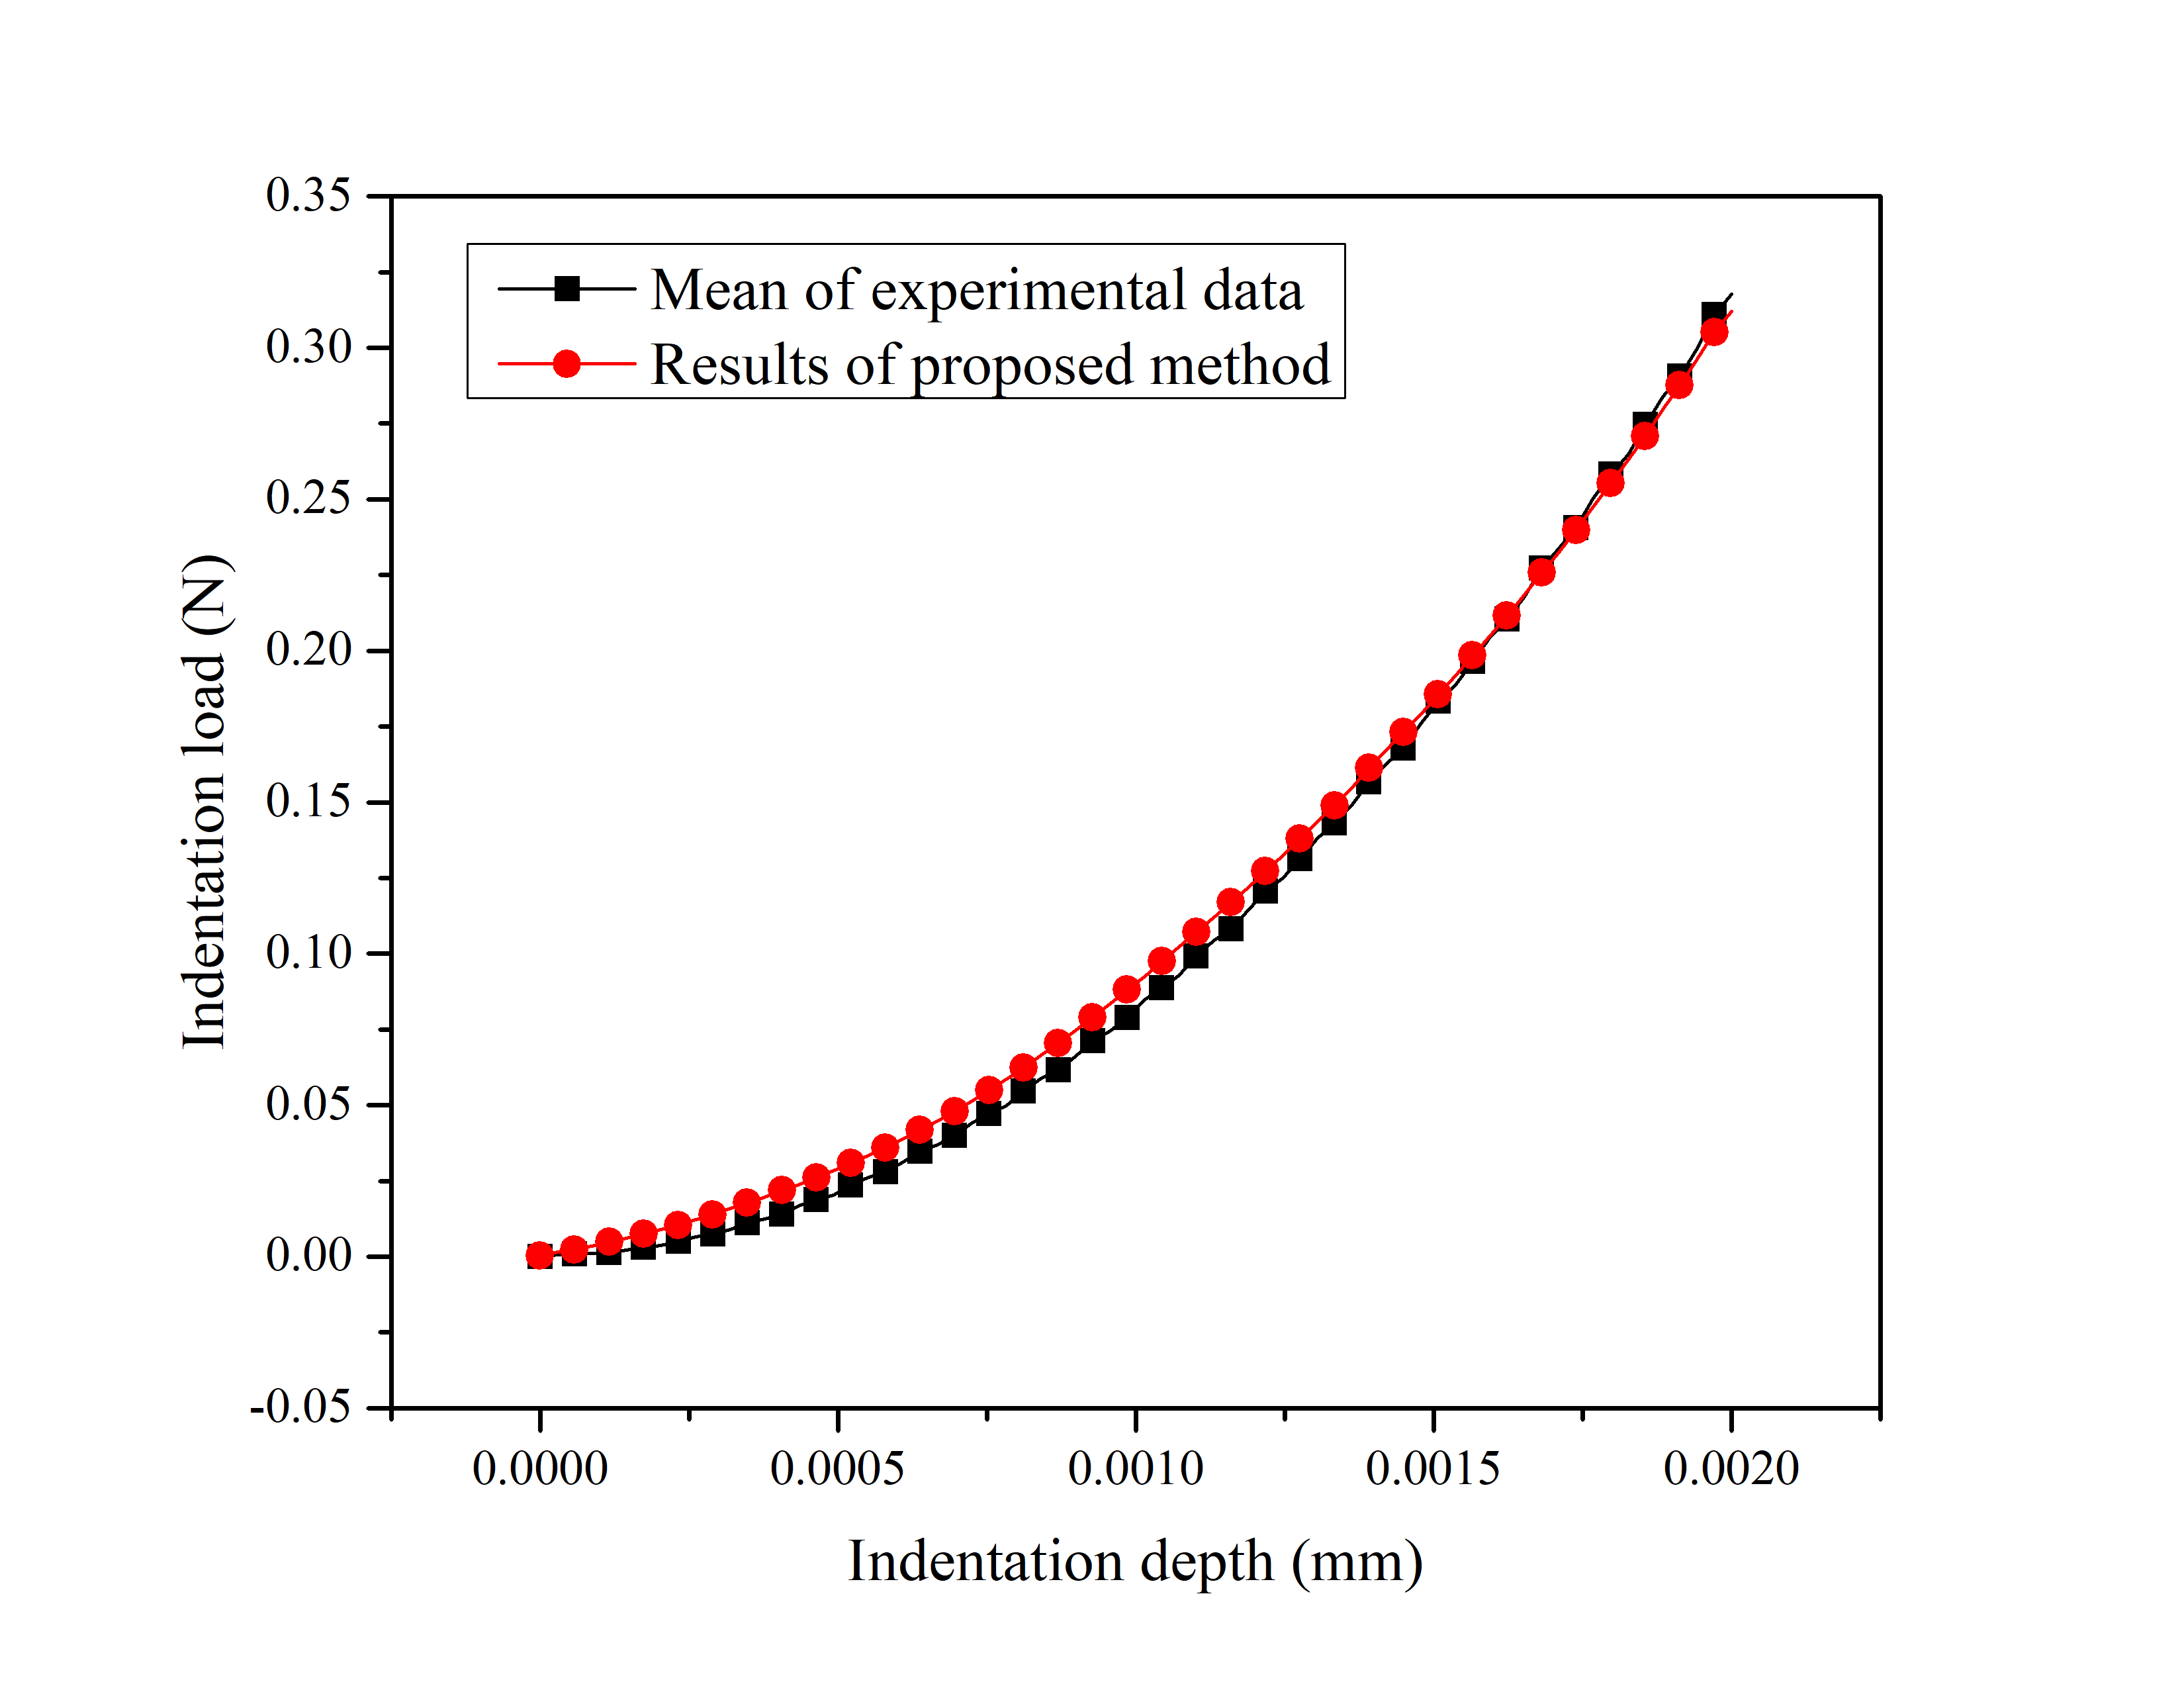
\includegraphics[width=0.45\textwidth]{./figs/result_B.png}}
\subfloat[Region C]{
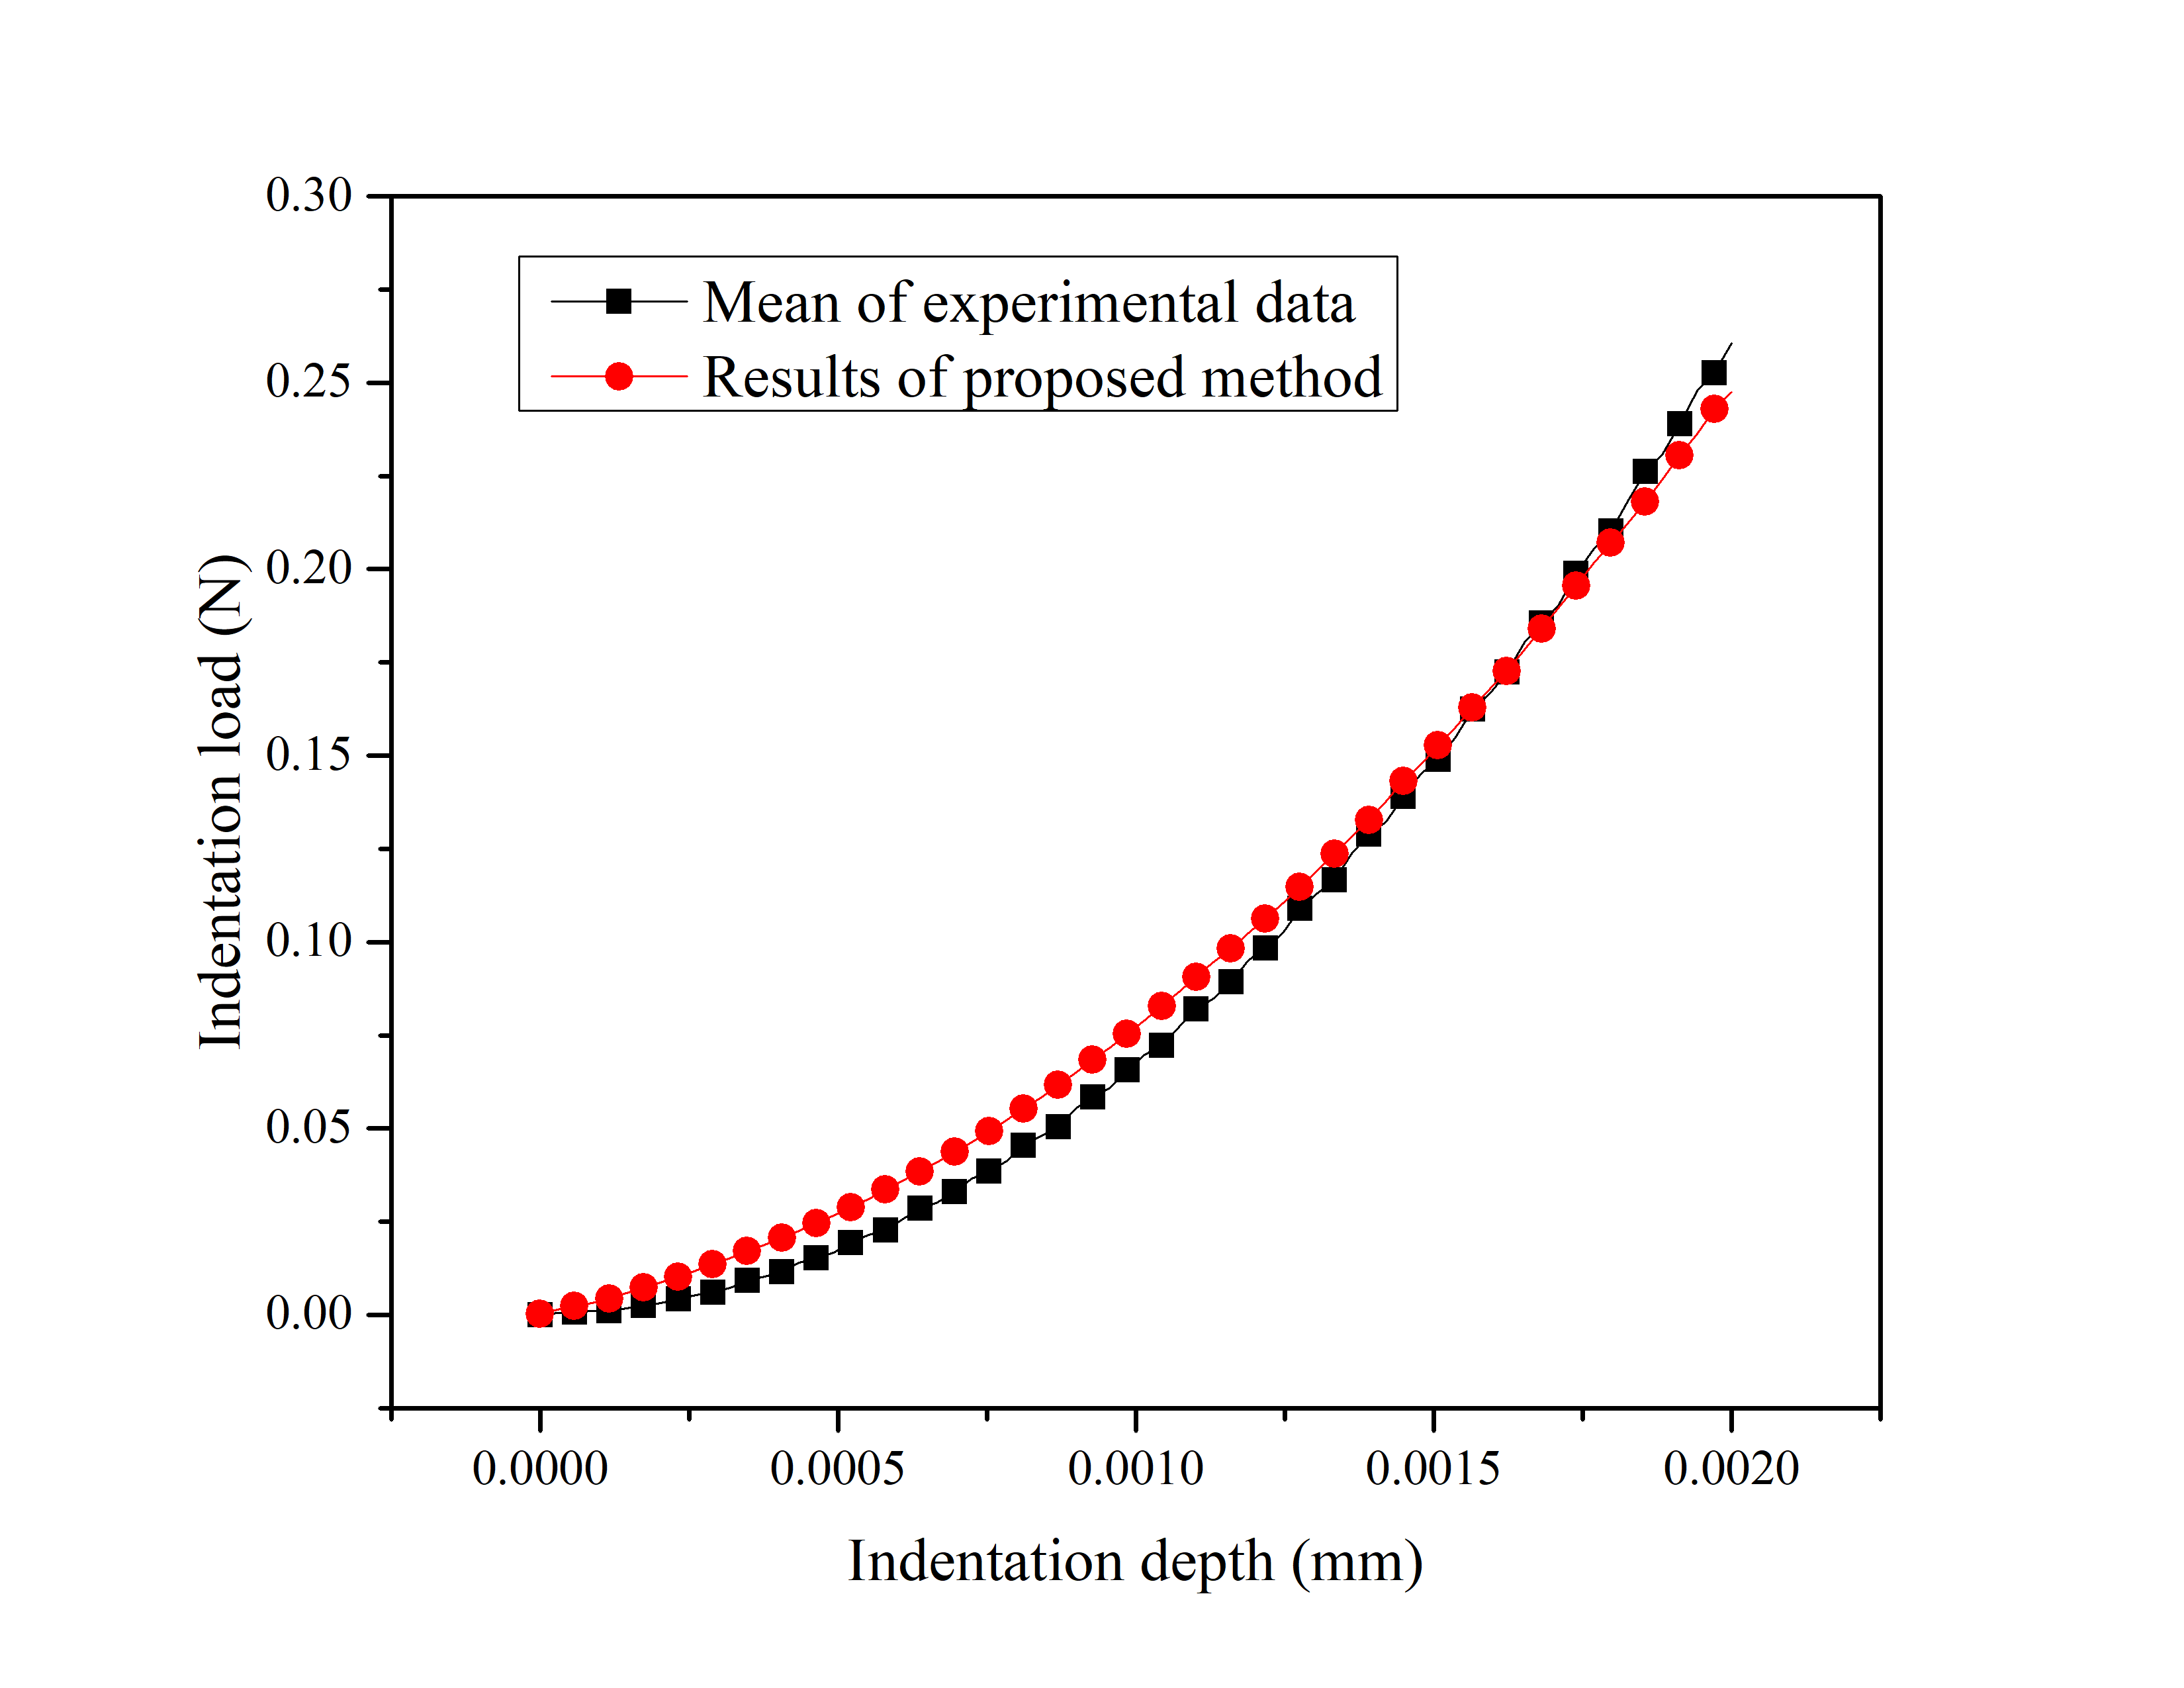
\includegraphics[width=0.45\textwidth]{./figs/result_C.png}}
\caption{The comparison between means of posteriors and means of experimental data}
\label{fig:comparison regions}
\end{figure}

\begin{figure}[h!]
    \centering
    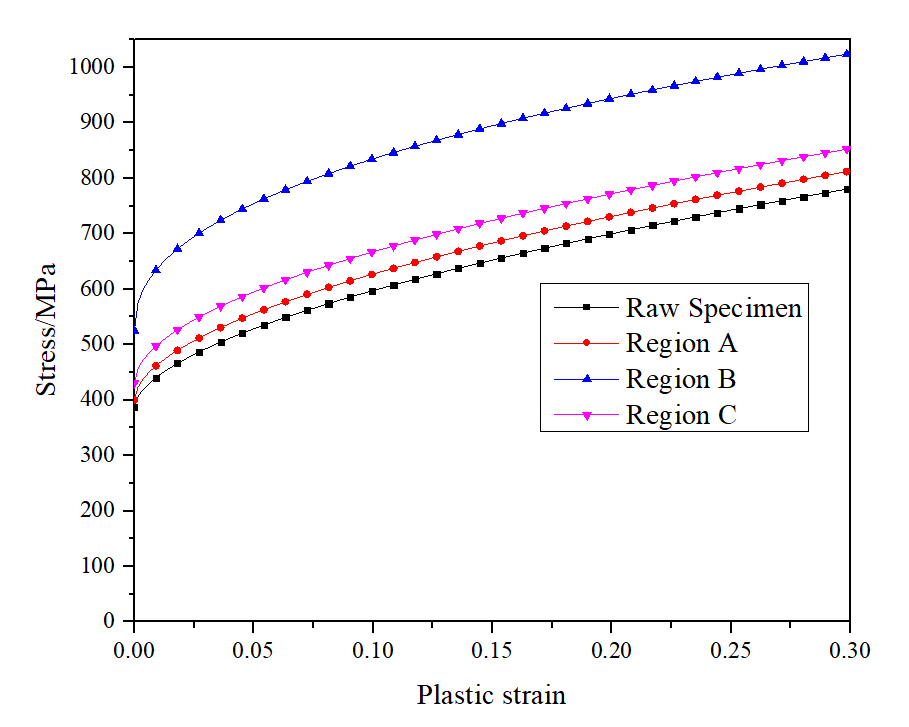
\includegraphics[width=0.6\textwidth]{figs/JCcurveresults.png}
    \caption{The stress-plastic strain curve of the indentation results}
    \label{fig:plasticresults}
\end{figure}

To compare the material properties of raw and formed specimen clearly, the means and standard deviations of posteriors are presented in Table.~\ref{table:results}. \textcolor{black}{The plastic strain-stress curves of these means are presented in Fig.~\ref{fig:plasticresults}.} From the results presented in Table.~\ref{table:results} and Fig.~\ref{fig:plasticresults}, it is obvious that forming has a considerable influence on the material properties which is consistent with the value of hardness. In region A, all the value of hardness in region A are closer to the curve of the raw specimens than that in the other region. The corresponding P-h curves shows the same feature. Thus leads a small variant of the posteriori material parameters in this region. The material properties in region B have a relatively larger difference with the material properties of raw specimen. This is also consistent with the value of hardness. As for the region C, the variant of material parameters is between that in region A and B. More deformation of forming leads to more various of material parameters. It makes senses in physics.

The yield strength $\mathbf{A}$ and modulus of strain hardening $\mathbf{B}$ are improved in varying degrees due to cold hardening after forming as shown in Table.\ref{table:results}. Due to the main deformation, the yield strength and modulus of strain hardening in region B are improved more than that in region A and C. The hardening coefficient $\mathbf{n}$ are decreased after forming. The large deformation may also lead to more decreased strain hardening shown in regions B. 

\textcolor{black}{
Here in order to validate the results of indentation tests, a tensile test is presented with the raw specimen as shown in Fig.\ref{fig:measuredtension}. Via comparing the results from tensile test and indentation tests of raw specimen, the results of indentation tests can be validated. The true stress-strain curve of tensile test is presented in Fig.\ref{fig:tensile}a. The stress-plastic strain curves of tensile test, fitted JC model with tensile test and indentation tests are presented in Fig.\ref{fig:tensile}b. With fitting the tensile test to JC model (red line in Fig.\ref{fig:tensile}b), we can obtain $\mathbf{A} = 397.4$, $\mathbf{B}=798.21$ and $\mathbf{n}=0.543$. The results of indentation tests of the raw specimen which are $\mathbf{A} = 387.1$, $\mathbf{B}=785.6$ and $\mathbf{n}=0.57$. The maximum different value among these curves is 4.48\%. Due to different experimental condition, this value is acceptable. It proves that the results of indentation tests are acceptable.
}

\begin{figure}[h]
\centering
\subfloat[The true stress-strain curve of tensile test]{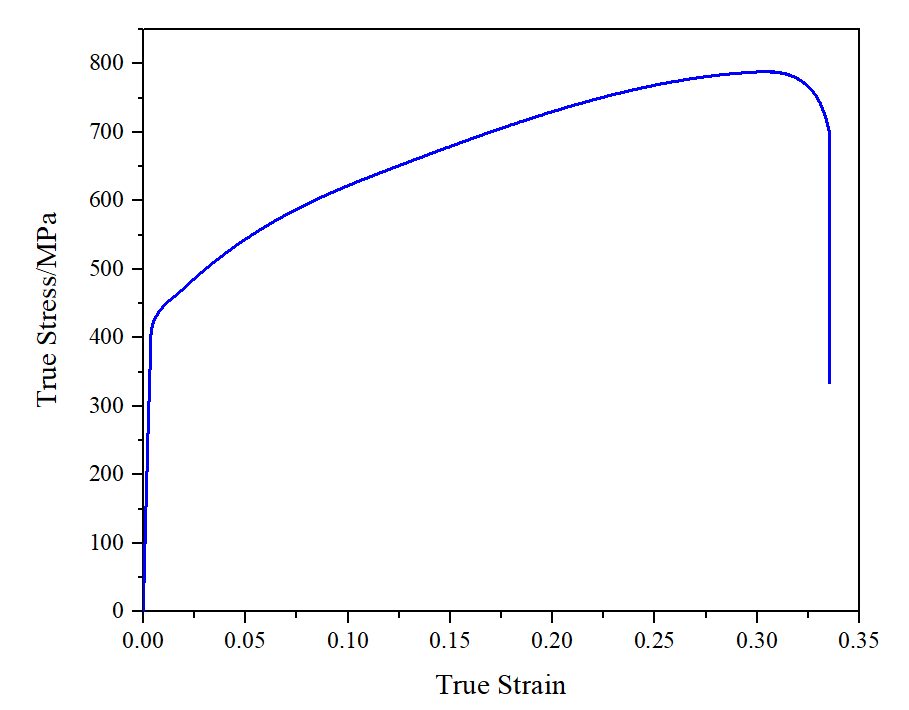
\includegraphics[width=0.44\textwidth]{./figs/tensile_true.png}}
\subfloat[Comparison of tensile test and indentation test]{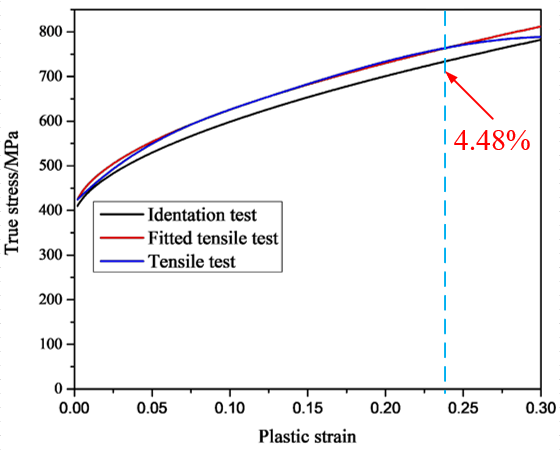
\includegraphics[width=0.41\textwidth]{./figs/tensile-indentation.png}}

\caption{Verify the results of indentation test with tensile test}
\label{fig:tensile}
\end{figure}

\subsection{Verify the results with DIC}

To verify the results identified before, the formed specimen is tested on the universal testing machine (INSTRON 5985, USA) and DIC is equipped to detect the local deformation of the specimen. The FE models of formed specimen are constructed as shown in Fig.~\ref{fig:DIC-FE}. The specimen partitioned into different regions based on the value of hardness in Fig.\ref{fig:hardness} is presented in Fig.~\ref{fig:DIC-FE}a. The specimen with raw material parameters as shown in Fig.\ref{fig:DIC-FE}b is used as a benchmark. 

The force-displacement curves of simulations and test are presented in Fig.\ref{fig:verify}. According to it, it can be found that these curves can be divided into three stages. The first stage is that the curving specimen is straightened. In this stage, the bending stiffness of the specimen is mainly factor of resisting deformation. From Fig.\ref{fig:verify}, at the first stage, the slope of the force-displacement curves is small. A small load can lead to considerable displacement. The second stage is the elastic stage. In this stage, the specimen is almost straightened. The elastic deformation is the main part of deformation. Small increment of deformation needs large variant of load. The last stage is the hardening stage. In this stage, plastic deformation is the main factor. From Fig.\ref{fig:verify}, it can be seen that the results obtained from partitioned FE simulation are more accurate than no-partitioned FE simulation in elastic and plastic deformation. In the elastic stage, it shows that the force-displacement curves have almost the same slope. This results from the same elastic modulus. Cold hardening has little influence on elastic modulus. However, the partitioned and experimental curve is higher than that of no-partitioned FE model. This is because in the elastic stage, due to the curving of specimen, some little plastic deformation happened. In the plastic stage, it is obviously that the force-displacement curve of partitioned is much higher than the no-partitioned one due to the larger yield strength and higher hardening modulus after cold hardening. \textcolor{black}{The partitioned FE model fares better in the plastic stage than the no-partitioned one.} 

\textcolor{black}{Since the main difference of results happens in the plastic stage as shown in Fig.\ref{fig:verify}, the contour of strains in the plastic stage is used to prove the local performance of partitioned FE simulation. The contour of strains at displacement of 9mm is presented in Fig.~\ref{fig:DICresults}. From them, it can be seen that the contour of strains of partitioned FE simulation are entirely more consistent with the DIC results than the no-partitioned one. Since the homogeneous material parameters are used in the no-partitioned FE model, the fluctuation of its contour of strains are much smaller than the partitioned one and DIC test. The strains in region B and C of partitioned FE model and test are smaller than that of the no-partitioned FE model. It makes sense since after forming the material properties of these regions are strengthened a lot. Thus, for the same stress, region B has smaller plastic strains. It leads to more strains in the other regions to keep the same displacement. The strains in region A of partitioned FE model and test are larger than that of the no-partitioned FE model. It proves that the partitioned FE model has a better local behavior of specimen in the plastic deformation process. Since means of material parameters in regions are used, the FE results is still conservative. In conclusion, the Fig.~\ref{fig:DICresults} combined with Fig.~\ref{fig:verify} prove that partitioned FE model show a better local and global material behavior than the no-partitioned one.}

\begin{figure}[h!]
\centering
\subfloat[The FE model of partitioned specimen]{
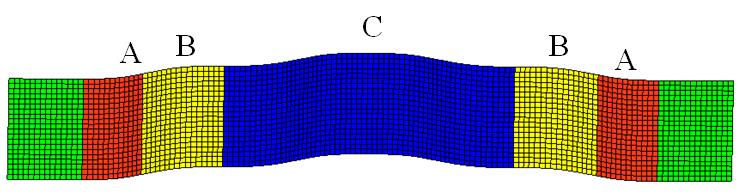
\includegraphics[width=0.85\textwidth]{./figs/partitionmesh.jpg}
}

\subfloat[The FE model of non-partitioned specimen]{
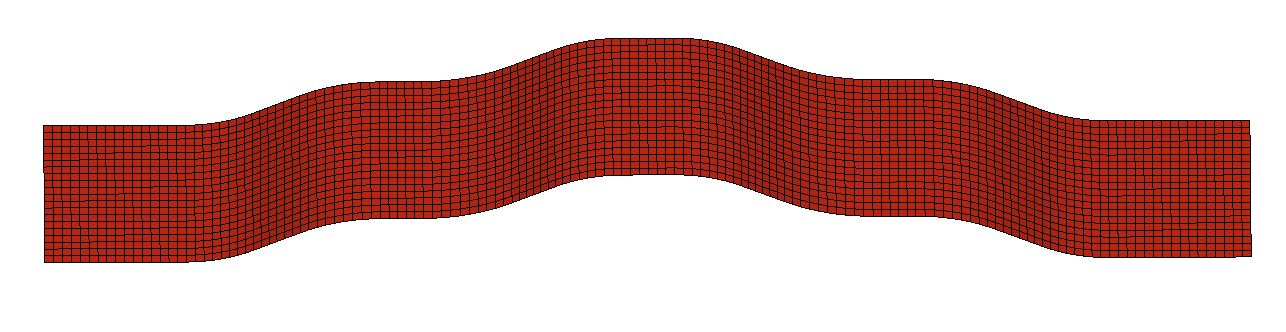
\includegraphics[width=0.9\textwidth]{./figs/non-partitioned.png}}
\caption{The FE model of DIC specimen}
\label{fig:DIC-FE}
\end{figure}

\begin{figure}[h!]
\centering
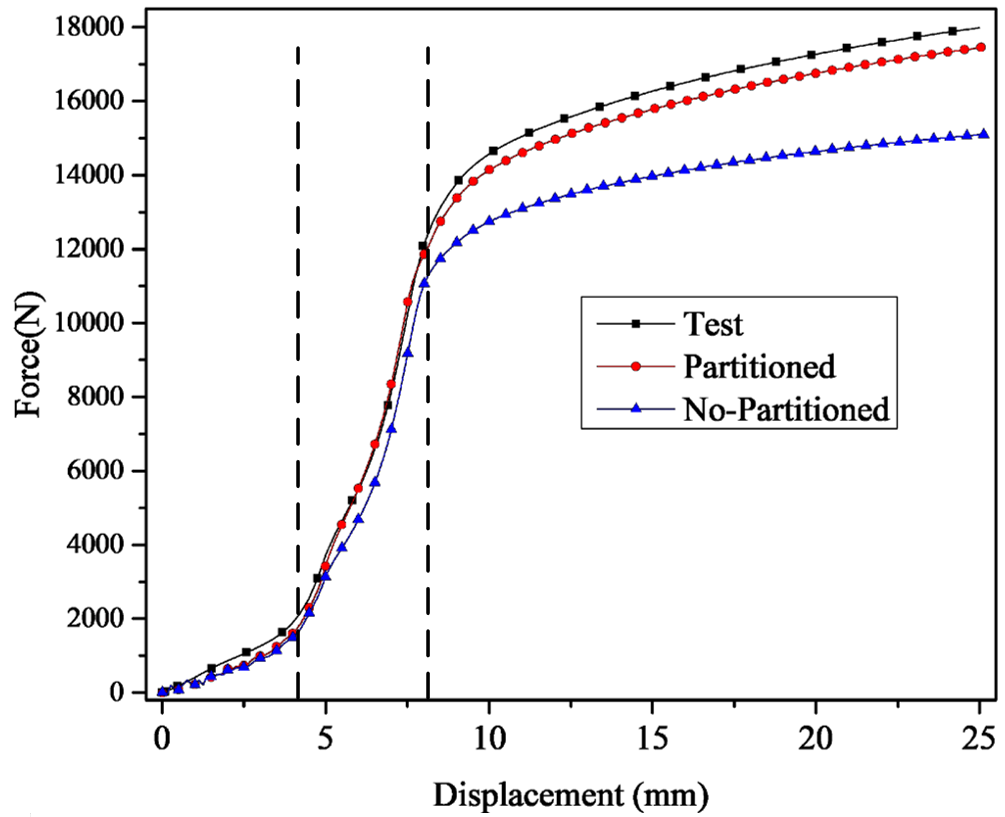
\includegraphics[width=0.8\textwidth]{./figs/DICverify.png}
\caption{The force-displacement curve of DIC test and FE simulations}
\label{fig:verify}
\end{figure}

\begin{figure}[h!]
\centering
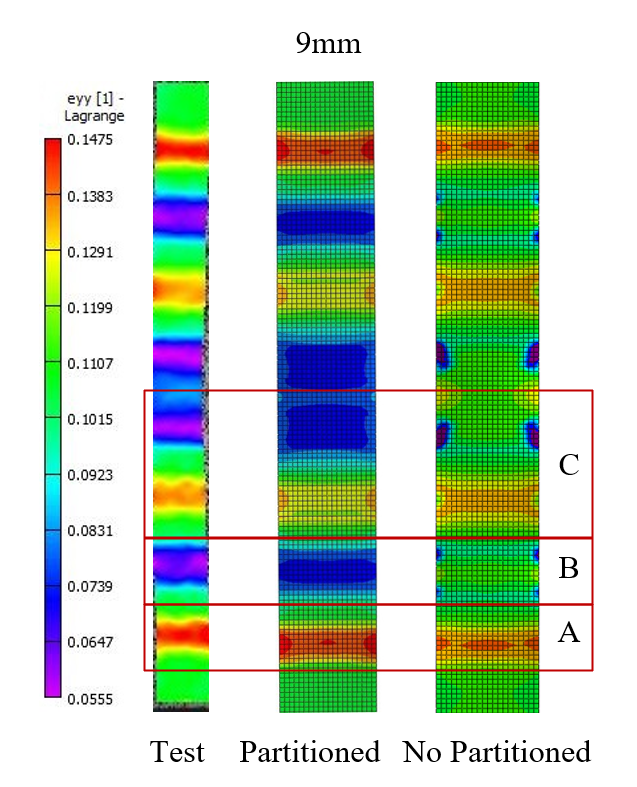
\includegraphics[width=0.8\textwidth]{figs/DIC_FEM_modified.png}
\caption{The DIC results and FEM contour of strains}
\label{fig:DICresults}
\end{figure}

\section{Conclusion}

A comprehensive study of influence of formed on material properties is presented. Indentation test is used to measure the local material properties affected by forming. In order to figure out the influence of the material properties from forming, the specimens without formed are also implemented with indentation test to present comparison with formed specimen. A new flexible POD-based ABC method is proposed to address the ill-posed indentation test. In the end, a DIC experiment is presented to verify the effectiveness of designed experiment and proposed methods. From the results, several conclusion can be obtained:

\begin{itemize}
\item The forming has considerable influence on material properties.
\item The proposed method is flexible and feasible for the parameter identification.
\item In order to obtain accurate FE simulation, dividing the formed steel to small region with local material properties is a good choice.
\end{itemize}


\section*{Acknownadge}

This work has been supported by Project of the Key Program of National Natural Science Foundation of China under the Grant Numbers 11572120, National Key Research and Development Program of China 2017YFB0203701.\



\section*{Reference}

\bibliographystyle{elsarticle-num}
\bibliography{mybibfile}

\end{document}